\textcolor{teal}{\textbf{solution idea.}} We distinguish between uncertain subgraphs and neutral subgraphs devoid of any uncertainty. Shortest-path algorithms are queried on uncertain subgraphs. A fast subroutine searches for paths among the neutral zone, connecting those uncertain subgraphs with each other. Combining computed paths of uncertain zones and neutral zones is realized by constructing a smaller higher-level graph as in \textit{Figure (3-4)}. Finding a shortest-path of it, accounts for both uncertain subgraphs and neutral subgraphs, minimizing total expectation. Any black-box shortest-path subroutine could be used, and the choice of it is out of this paper's scope. Dynamic updates follow the basic idea of avoiding recomputing a path from $s$ to $d$ if all intermediary vertices are unchanged. If an object's subgraph probabilities change, then the higher-level graph will correspondingly change, requiring only re-querying shortest-path subroutine on the smaller higher-level graph, utilizing all what was previously computed. If an object's diameter changes, a new object appears or disappears, then a single vertex of the higher-level graph will correspondingly change. The faster neutral path gets re-queried, then again we look for a better path on the higher-level graph. In all cases, expensive computations of uncertain subgraphs shortest-paths are re-utilized. Tackling vertex weights is not common in the literature. Notable rare examples are \cite{vertexWeighted_1}, \cite{vertexWeighted_2}, and \cite{vertexWeighted_3}.

\textcolor{teal}{\textbf{intuitive example on figure 3.}} Let's reflect that on a concrete example of \textit{Figure 3}. (1) is the given input graph. For an uncertain subgraph, (2) reduces the shortest path from a starting vertex to a destination vertex, to a single weighted edge. (3) transforms every source-destination pair to a single vertex. (4) queries the faster neutral path mechanism, to find arbitrary paths between the yellow highlighted vertices. Resulting edges are not weighted since selecting which neutral path to take has nothing to do with minimizing expected harm. Now we are given a vertex-weighted graph again, so we can query shortest-path on it in (5). As seen in (6), the path computed in (5), alongside neutral paths, and shortest-paths computed earlier, are all combined to produce the final optimal path of (1).

\tikzset{every picture/.style={line width=0.75pt}} %set default line width to 0.75pt  

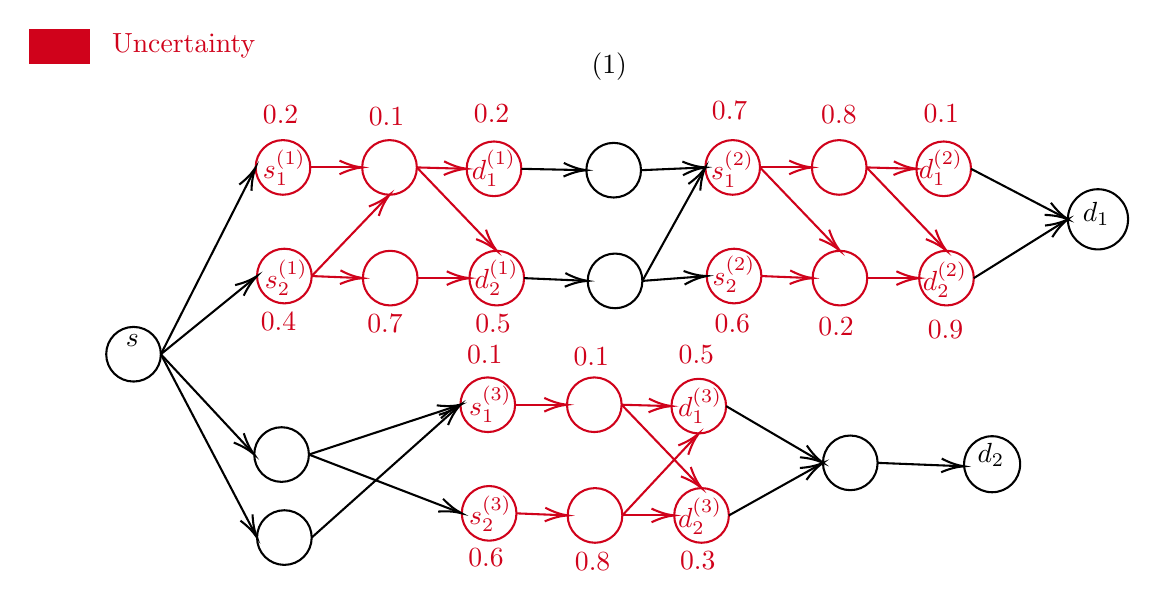
\begin{tikzpicture}[x=0.75pt,y=0.75pt,yscale=-1,xscale=1]
%uncomment if require: \path (0,293); %set diagram left start at 0, and has height of 293

%Shape: Circle [id:dp8991053355567844] 
\draw   (99.67,166.83) .. controls (99.67,159.56) and (105.56,153.67) .. (112.83,153.67) .. controls (120.11,153.67) and (126,159.56) .. (126,166.83) .. controls (126,174.11) and (120.11,180) .. (112.83,180) .. controls (105.56,180) and (99.67,174.11) .. (99.67,166.83) -- cycle ;
%Shape: Circle [id:dp6667370209216856] 
\draw   (563,101.83) .. controls (563,93.83) and (569.49,87.33) .. (577.5,87.33) .. controls (585.51,87.33) and (592,93.83) .. (592,101.83) .. controls (592,109.84) and (585.51,116.33) .. (577.5,116.33) .. controls (569.49,116.33) and (563,109.84) .. (563,101.83) -- cycle ;
%Shape: Circle [id:dp7692416494148475] 
\draw   (513,219.83) .. controls (513,212.38) and (519.04,206.33) .. (526.5,206.33) .. controls (533.96,206.33) and (540,212.38) .. (540,219.83) .. controls (540,227.29) and (533.96,233.33) .. (526.5,233.33) .. controls (519.04,233.33) and (513,227.29) .. (513,219.83) -- cycle ;
%Shape: Circle [id:dp21154466512128334] 
\draw  [color={rgb, 255:red, 208; green, 2; blue, 27 }  ,draw opacity=1 ] (171.67,76.83) .. controls (171.67,69.56) and (177.56,63.67) .. (184.83,63.67) .. controls (192.11,63.67) and (198,69.56) .. (198,76.83) .. controls (198,84.11) and (192.11,90) .. (184.83,90) .. controls (177.56,90) and (171.67,84.11) .. (171.67,76.83) -- cycle ;
%Shape: Circle [id:dp8549674263314191] 
\draw  [color={rgb, 255:red, 208; green, 2; blue, 27 }  ,draw opacity=1 ] (223,76.83) .. controls (223,69.56) and (228.89,63.67) .. (236.17,63.67) .. controls (243.44,63.67) and (249.33,69.56) .. (249.33,76.83) .. controls (249.33,84.11) and (243.44,90) .. (236.17,90) .. controls (228.89,90) and (223,84.11) .. (223,76.83) -- cycle ;
%Shape: Circle [id:dp5177282977671258] 
\draw  [color={rgb, 255:red, 208; green, 2; blue, 27 }  ,draw opacity=1 ] (273.33,77.5) .. controls (273.33,70.23) and (279.23,64.33) .. (286.5,64.33) .. controls (293.77,64.33) and (299.67,70.23) .. (299.67,77.5) .. controls (299.67,84.77) and (293.77,90.67) .. (286.5,90.67) .. controls (279.23,90.67) and (273.33,84.77) .. (273.33,77.5) -- cycle ;
%Shape: Circle [id:dp8008697844392914] 
\draw  [color={rgb, 255:red, 208; green, 2; blue, 27 }  ,draw opacity=1 ] (172.33,129.17) .. controls (172.33,121.89) and (178.23,116) .. (185.5,116) .. controls (192.77,116) and (198.67,121.89) .. (198.67,129.17) .. controls (198.67,136.44) and (192.77,142.33) .. (185.5,142.33) .. controls (178.23,142.33) and (172.33,136.44) .. (172.33,129.17) -- cycle ;
%Shape: Circle [id:dp9896153955397202] 
\draw  [color={rgb, 255:red, 208; green, 2; blue, 27 }  ,draw opacity=1 ] (223.33,130.17) .. controls (223.33,122.89) and (229.23,117) .. (236.5,117) .. controls (243.77,117) and (249.67,122.89) .. (249.67,130.17) .. controls (249.67,137.44) and (243.77,143.33) .. (236.5,143.33) .. controls (229.23,143.33) and (223.33,137.44) .. (223.33,130.17) -- cycle ;
%Shape: Circle [id:dp7468151230781632] 
\draw  [color={rgb, 255:red, 208; green, 2; blue, 27 }  ,draw opacity=1 ] (274.67,130.17) .. controls (274.67,122.89) and (280.56,117) .. (287.83,117) .. controls (295.11,117) and (301,122.89) .. (301,130.17) .. controls (301,137.44) and (295.11,143.33) .. (287.83,143.33) .. controls (280.56,143.33) and (274.67,137.44) .. (274.67,130.17) -- cycle ;
%Straight Lines [id:da28707798144000396] 
\draw [color={rgb, 255:red, 208; green, 2; blue, 27 }  ,draw opacity=1 ]   (198,76.83) -- (221,76.83) ;
\draw [shift={(223,76.83)}, rotate = 180] [color={rgb, 255:red, 208; green, 2; blue, 27 }  ,draw opacity=1 ][line width=0.75]    (10.93,-3.29) .. controls (6.95,-1.4) and (3.31,-0.3) .. (0,0) .. controls (3.31,0.3) and (6.95,1.4) .. (10.93,3.29)   ;
%Straight Lines [id:da09837669241456393] 
\draw [color={rgb, 255:red, 208; green, 2; blue, 27 }  ,draw opacity=1 ]   (249.33,76.83) -- (271.33,77.44) ;
\draw [shift={(273.33,77.5)}, rotate = 181.59] [color={rgb, 255:red, 208; green, 2; blue, 27 }  ,draw opacity=1 ][line width=0.75]    (10.93,-3.29) .. controls (6.95,-1.4) and (3.31,-0.3) .. (0,0) .. controls (3.31,0.3) and (6.95,1.4) .. (10.93,3.29)   ;
%Straight Lines [id:da5277927281771255] 
\draw [color={rgb, 255:red, 208; green, 2; blue, 27 }  ,draw opacity=1 ]   (198.67,129.17) -- (221.33,130.09) ;
\draw [shift={(223.33,130.17)}, rotate = 182.32] [color={rgb, 255:red, 208; green, 2; blue, 27 }  ,draw opacity=1 ][line width=0.75]    (10.93,-3.29) .. controls (6.95,-1.4) and (3.31,-0.3) .. (0,0) .. controls (3.31,0.3) and (6.95,1.4) .. (10.93,3.29)   ;
%Straight Lines [id:da7957518998165858] 
\draw [color={rgb, 255:red, 208; green, 2; blue, 27 }  ,draw opacity=1 ]   (249.67,130.17) -- (272.67,130.17) ;
\draw [shift={(274.67,130.17)}, rotate = 180] [color={rgb, 255:red, 208; green, 2; blue, 27 }  ,draw opacity=1 ][line width=0.75]    (10.93,-3.29) .. controls (6.95,-1.4) and (3.31,-0.3) .. (0,0) .. controls (3.31,0.3) and (6.95,1.4) .. (10.93,3.29)   ;
%Straight Lines [id:da6087292877067254] 
\draw [color={rgb, 255:red, 208; green, 2; blue, 27 }  ,draw opacity=1 ]   (249.33,76.83) -- (286.45,115.56) ;
\draw [shift={(287.83,117)}, rotate = 226.21] [color={rgb, 255:red, 208; green, 2; blue, 27 }  ,draw opacity=1 ][line width=0.75]    (10.93,-3.29) .. controls (6.95,-1.4) and (3.31,-0.3) .. (0,0) .. controls (3.31,0.3) and (6.95,1.4) .. (10.93,3.29)   ;
%Straight Lines [id:da20773980392742475] 
\draw [color={rgb, 255:red, 208; green, 2; blue, 27 }  ,draw opacity=1 ]   (198.67,129.17) -- (234.78,91.44) ;
\draw [shift={(236.17,90)}, rotate = 133.75] [color={rgb, 255:red, 208; green, 2; blue, 27 }  ,draw opacity=1 ][line width=0.75]    (10.93,-3.29) .. controls (6.95,-1.4) and (3.31,-0.3) .. (0,0) .. controls (3.31,0.3) and (6.95,1.4) .. (10.93,3.29)   ;
%Shape: Circle [id:dp605117679807236] 
\draw  [color={rgb, 255:red, 208; green, 2; blue, 27 }  ,draw opacity=1 ] (388.33,76.83) .. controls (388.33,69.56) and (394.23,63.67) .. (401.5,63.67) .. controls (408.77,63.67) and (414.67,69.56) .. (414.67,76.83) .. controls (414.67,84.11) and (408.77,90) .. (401.5,90) .. controls (394.23,90) and (388.33,84.11) .. (388.33,76.83) -- cycle ;
%Shape: Circle [id:dp5025593038685328] 
\draw  [color={rgb, 255:red, 208; green, 2; blue, 27 }  ,draw opacity=1 ] (439.67,76.83) .. controls (439.67,69.56) and (445.56,63.67) .. (452.83,63.67) .. controls (460.11,63.67) and (466,69.56) .. (466,76.83) .. controls (466,84.11) and (460.11,90) .. (452.83,90) .. controls (445.56,90) and (439.67,84.11) .. (439.67,76.83) -- cycle ;
%Shape: Circle [id:dp1597676513079207] 
\draw  [color={rgb, 255:red, 208; green, 2; blue, 27 }  ,draw opacity=1 ] (490,77.5) .. controls (490,70.23) and (495.89,64.33) .. (503.17,64.33) .. controls (510.44,64.33) and (516.33,70.23) .. (516.33,77.5) .. controls (516.33,84.77) and (510.44,90.67) .. (503.17,90.67) .. controls (495.89,90.67) and (490,84.77) .. (490,77.5) -- cycle ;
%Shape: Circle [id:dp2458439574961957] 
\draw  [color={rgb, 255:red, 208; green, 2; blue, 27 }  ,draw opacity=1 ] (389,129.17) .. controls (389,121.89) and (394.89,116) .. (402.17,116) .. controls (409.44,116) and (415.33,121.89) .. (415.33,129.17) .. controls (415.33,136.44) and (409.44,142.33) .. (402.17,142.33) .. controls (394.89,142.33) and (389,136.44) .. (389,129.17) -- cycle ;
%Shape: Circle [id:dp2635994355412301] 
\draw  [color={rgb, 255:red, 208; green, 2; blue, 27 }  ,draw opacity=1 ] (440,130.17) .. controls (440,122.89) and (445.89,117) .. (453.17,117) .. controls (460.44,117) and (466.33,122.89) .. (466.33,130.17) .. controls (466.33,137.44) and (460.44,143.33) .. (453.17,143.33) .. controls (445.89,143.33) and (440,137.44) .. (440,130.17) -- cycle ;
%Shape: Circle [id:dp2585338650889719] 
\draw  [color={rgb, 255:red, 208; green, 2; blue, 27 }  ,draw opacity=1 ] (491.33,130.17) .. controls (491.33,122.89) and (497.23,117) .. (504.5,117) .. controls (511.77,117) and (517.67,122.89) .. (517.67,130.17) .. controls (517.67,137.44) and (511.77,143.33) .. (504.5,143.33) .. controls (497.23,143.33) and (491.33,137.44) .. (491.33,130.17) -- cycle ;
%Straight Lines [id:da3420914815638465] 
\draw [color={rgb, 255:red, 208; green, 2; blue, 27 }  ,draw opacity=1 ]   (414.67,76.83) -- (437.67,76.83) ;
\draw [shift={(439.67,76.83)}, rotate = 180] [color={rgb, 255:red, 208; green, 2; blue, 27 }  ,draw opacity=1 ][line width=0.75]    (10.93,-3.29) .. controls (6.95,-1.4) and (3.31,-0.3) .. (0,0) .. controls (3.31,0.3) and (6.95,1.4) .. (10.93,3.29)   ;
%Straight Lines [id:da12524774189704457] 
\draw [color={rgb, 255:red, 208; green, 2; blue, 27 }  ,draw opacity=1 ]   (466,76.83) -- (488,77.44) ;
\draw [shift={(490,77.5)}, rotate = 181.59] [color={rgb, 255:red, 208; green, 2; blue, 27 }  ,draw opacity=1 ][line width=0.75]    (10.93,-3.29) .. controls (6.95,-1.4) and (3.31,-0.3) .. (0,0) .. controls (3.31,0.3) and (6.95,1.4) .. (10.93,3.29)   ;
%Straight Lines [id:da5006368121447826] 
\draw [color={rgb, 255:red, 208; green, 2; blue, 27 }  ,draw opacity=1 ]   (415.33,129.17) -- (438,130.09) ;
\draw [shift={(440,130.17)}, rotate = 182.32] [color={rgb, 255:red, 208; green, 2; blue, 27 }  ,draw opacity=1 ][line width=0.75]    (10.93,-3.29) .. controls (6.95,-1.4) and (3.31,-0.3) .. (0,0) .. controls (3.31,0.3) and (6.95,1.4) .. (10.93,3.29)   ;
%Straight Lines [id:da5861207499216747] 
\draw [color={rgb, 255:red, 208; green, 2; blue, 27 }  ,draw opacity=1 ]   (466.33,130.17) -- (489.33,130.17) ;
\draw [shift={(491.33,130.17)}, rotate = 180] [color={rgb, 255:red, 208; green, 2; blue, 27 }  ,draw opacity=1 ][line width=0.75]    (10.93,-3.29) .. controls (6.95,-1.4) and (3.31,-0.3) .. (0,0) .. controls (3.31,0.3) and (6.95,1.4) .. (10.93,3.29)   ;
%Straight Lines [id:da48440127546935496] 
\draw [color={rgb, 255:red, 208; green, 2; blue, 27 }  ,draw opacity=1 ]   (414.67,76.83) -- (451.78,115.56) ;
\draw [shift={(453.17,117)}, rotate = 226.21] [color={rgb, 255:red, 208; green, 2; blue, 27 }  ,draw opacity=1 ][line width=0.75]    (10.93,-3.29) .. controls (6.95,-1.4) and (3.31,-0.3) .. (0,0) .. controls (3.31,0.3) and (6.95,1.4) .. (10.93,3.29)   ;
%Straight Lines [id:da3339624104323835] 
\draw [color={rgb, 255:red, 208; green, 2; blue, 27 }  ,draw opacity=1 ]   (466,76.83) -- (503.12,115.56) ;
\draw [shift={(504.5,117)}, rotate = 226.21] [color={rgb, 255:red, 208; green, 2; blue, 27 }  ,draw opacity=1 ][line width=0.75]    (10.93,-3.29) .. controls (6.95,-1.4) and (3.31,-0.3) .. (0,0) .. controls (3.31,0.3) and (6.95,1.4) .. (10.93,3.29)   ;
%Shape: Circle [id:dp34260775943439925] 
\draw  [color={rgb, 255:red, 208; green, 2; blue, 27 }  ,draw opacity=1 ] (270.33,191.17) .. controls (270.33,183.89) and (276.23,178) .. (283.5,178) .. controls (290.77,178) and (296.67,183.89) .. (296.67,191.17) .. controls (296.67,198.44) and (290.77,204.33) .. (283.5,204.33) .. controls (276.23,204.33) and (270.33,198.44) .. (270.33,191.17) -- cycle ;
%Shape: Circle [id:dp26682292157661114] 
\draw  [color={rgb, 255:red, 208; green, 2; blue, 27 }  ,draw opacity=1 ] (321.67,191.17) .. controls (321.67,183.89) and (327.56,178) .. (334.83,178) .. controls (342.11,178) and (348,183.89) .. (348,191.17) .. controls (348,198.44) and (342.11,204.33) .. (334.83,204.33) .. controls (327.56,204.33) and (321.67,198.44) .. (321.67,191.17) -- cycle ;
%Shape: Circle [id:dp3609359635117986] 
\draw  [color={rgb, 255:red, 208; green, 2; blue, 27 }  ,draw opacity=1 ] (372,191.83) .. controls (372,184.56) and (377.89,178.67) .. (385.17,178.67) .. controls (392.44,178.67) and (398.33,184.56) .. (398.33,191.83) .. controls (398.33,199.11) and (392.44,205) .. (385.17,205) .. controls (377.89,205) and (372,199.11) .. (372,191.83) -- cycle ;
%Shape: Circle [id:dp8338002922740684] 
\draw  [color={rgb, 255:red, 208; green, 2; blue, 27 }  ,draw opacity=1 ] (271,243.5) .. controls (271,236.23) and (276.89,230.33) .. (284.17,230.33) .. controls (291.44,230.33) and (297.33,236.23) .. (297.33,243.5) .. controls (297.33,250.77) and (291.44,256.67) .. (284.17,256.67) .. controls (276.89,256.67) and (271,250.77) .. (271,243.5) -- cycle ;
%Shape: Circle [id:dp8844906592132518] 
\draw  [color={rgb, 255:red, 208; green, 2; blue, 27 }  ,draw opacity=1 ] (322,244.5) .. controls (322,237.23) and (327.89,231.33) .. (335.17,231.33) .. controls (342.44,231.33) and (348.33,237.23) .. (348.33,244.5) .. controls (348.33,251.77) and (342.44,257.67) .. (335.17,257.67) .. controls (327.89,257.67) and (322,251.77) .. (322,244.5) -- cycle ;
%Shape: Circle [id:dp3017118545884758] 
\draw  [color={rgb, 255:red, 208; green, 2; blue, 27 }  ,draw opacity=1 ] (373.33,244.5) .. controls (373.33,237.23) and (379.23,231.33) .. (386.5,231.33) .. controls (393.77,231.33) and (399.67,237.23) .. (399.67,244.5) .. controls (399.67,251.77) and (393.77,257.67) .. (386.5,257.67) .. controls (379.23,257.67) and (373.33,251.77) .. (373.33,244.5) -- cycle ;
%Straight Lines [id:da2162937633954034] 
\draw [color={rgb, 255:red, 208; green, 2; blue, 27 }  ,draw opacity=1 ]   (296.67,191.17) -- (319.67,191.17) ;
\draw [shift={(321.67,191.17)}, rotate = 180] [color={rgb, 255:red, 208; green, 2; blue, 27 }  ,draw opacity=1 ][line width=0.75]    (10.93,-3.29) .. controls (6.95,-1.4) and (3.31,-0.3) .. (0,0) .. controls (3.31,0.3) and (6.95,1.4) .. (10.93,3.29)   ;
%Straight Lines [id:da16996745107685984] 
\draw [color={rgb, 255:red, 208; green, 2; blue, 27 }  ,draw opacity=1 ]   (348,191.17) -- (370,191.78) ;
\draw [shift={(372,191.83)}, rotate = 181.59] [color={rgb, 255:red, 208; green, 2; blue, 27 }  ,draw opacity=1 ][line width=0.75]    (10.93,-3.29) .. controls (6.95,-1.4) and (3.31,-0.3) .. (0,0) .. controls (3.31,0.3) and (6.95,1.4) .. (10.93,3.29)   ;
%Straight Lines [id:da6753041372818314] 
\draw [color={rgb, 255:red, 208; green, 2; blue, 27 }  ,draw opacity=1 ]   (297.33,243.5) -- (320,244.42) ;
\draw [shift={(322,244.5)}, rotate = 182.32] [color={rgb, 255:red, 208; green, 2; blue, 27 }  ,draw opacity=1 ][line width=0.75]    (10.93,-3.29) .. controls (6.95,-1.4) and (3.31,-0.3) .. (0,0) .. controls (3.31,0.3) and (6.95,1.4) .. (10.93,3.29)   ;
%Straight Lines [id:da29665288914740806] 
\draw [color={rgb, 255:red, 208; green, 2; blue, 27 }  ,draw opacity=1 ]   (348.33,244.5) -- (371.33,244.5) ;
\draw [shift={(373.33,244.5)}, rotate = 180] [color={rgb, 255:red, 208; green, 2; blue, 27 }  ,draw opacity=1 ][line width=0.75]    (10.93,-3.29) .. controls (6.95,-1.4) and (3.31,-0.3) .. (0,0) .. controls (3.31,0.3) and (6.95,1.4) .. (10.93,3.29)   ;
%Straight Lines [id:da4178410368718086] 
\draw [color={rgb, 255:red, 208; green, 2; blue, 27 }  ,draw opacity=1 ]   (348,191.17) -- (385.12,229.89) ;
\draw [shift={(386.5,231.33)}, rotate = 226.21] [color={rgb, 255:red, 208; green, 2; blue, 27 }  ,draw opacity=1 ][line width=0.75]    (10.93,-3.29) .. controls (6.95,-1.4) and (3.31,-0.3) .. (0,0) .. controls (3.31,0.3) and (6.95,1.4) .. (10.93,3.29)   ;
%Straight Lines [id:da6306182014131307] 
\draw [color={rgb, 255:red, 208; green, 2; blue, 27 }  ,draw opacity=1 ]   (348.33,244.5) -- (383.8,206.46) ;
\draw [shift={(385.17,205)}, rotate = 133] [color={rgb, 255:red, 208; green, 2; blue, 27 }  ,draw opacity=1 ][line width=0.75]    (10.93,-3.29) .. controls (6.95,-1.4) and (3.31,-0.3) .. (0,0) .. controls (3.31,0.3) and (6.95,1.4) .. (10.93,3.29)   ;
%Shape: Circle [id:dp8748683094287648] 
\draw   (171,215.17) .. controls (171,207.89) and (176.89,202) .. (184.17,202) .. controls (191.44,202) and (197.33,207.89) .. (197.33,215.17) .. controls (197.33,222.44) and (191.44,228.33) .. (184.17,228.33) .. controls (176.89,228.33) and (171,222.44) .. (171,215.17) -- cycle ;
%Shape: Circle [id:dp07605772848189396] 
\draw   (331.67,131.5) .. controls (331.67,124.23) and (337.56,118.33) .. (344.83,118.33) .. controls (352.11,118.33) and (358,124.23) .. (358,131.5) .. controls (358,138.77) and (352.11,144.67) .. (344.83,144.67) .. controls (337.56,144.67) and (331.67,138.77) .. (331.67,131.5) -- cycle ;
%Shape: Circle [id:dp04008475567883307] 
\draw   (331,78.17) .. controls (331,70.89) and (336.89,65) .. (344.17,65) .. controls (351.44,65) and (357.33,70.89) .. (357.33,78.17) .. controls (357.33,85.44) and (351.44,91.33) .. (344.17,91.33) .. controls (336.89,91.33) and (331,85.44) .. (331,78.17) -- cycle ;
%Shape: Circle [id:dp5031413049648514] 
\draw   (445,219.17) .. controls (445,211.89) and (450.89,206) .. (458.17,206) .. controls (465.44,206) and (471.33,211.89) .. (471.33,219.17) .. controls (471.33,226.44) and (465.44,232.33) .. (458.17,232.33) .. controls (450.89,232.33) and (445,226.44) .. (445,219.17) -- cycle ;
%Straight Lines [id:da7549754335080963] 
\draw    (126,166.83) -- (170.76,78.62) ;
\draw [shift={(171.67,76.83)}, rotate = 116.9] [color={rgb, 255:red, 0; green, 0; blue, 0 }  ][line width=0.75]    (10.93,-3.29) .. controls (6.95,-1.4) and (3.31,-0.3) .. (0,0) .. controls (3.31,0.3) and (6.95,1.4) .. (10.93,3.29)   ;
%Straight Lines [id:da05534827592076774] 
\draw    (126,166.83) -- (170.78,130.43) ;
\draw [shift={(172.33,129.17)}, rotate = 140.89] [color={rgb, 255:red, 0; green, 0; blue, 0 }  ][line width=0.75]    (10.93,-3.29) .. controls (6.95,-1.4) and (3.31,-0.3) .. (0,0) .. controls (3.31,0.3) and (6.95,1.4) .. (10.93,3.29)   ;
%Straight Lines [id:da4417489275158206] 
\draw    (299.67,77.5) -- (329,78.12) ;
\draw [shift={(331,78.17)}, rotate = 181.22] [color={rgb, 255:red, 0; green, 0; blue, 0 }  ][line width=0.75]    (10.93,-3.29) .. controls (6.95,-1.4) and (3.31,-0.3) .. (0,0) .. controls (3.31,0.3) and (6.95,1.4) .. (10.93,3.29)   ;
%Straight Lines [id:da6395153922296584] 
\draw    (357.33,78.17) -- (386.34,76.92) ;
\draw [shift={(388.33,76.83)}, rotate = 177.54] [color={rgb, 255:red, 0; green, 0; blue, 0 }  ][line width=0.75]    (10.93,-3.29) .. controls (6.95,-1.4) and (3.31,-0.3) .. (0,0) .. controls (3.31,0.3) and (6.95,1.4) .. (10.93,3.29)   ;
%Straight Lines [id:da7289363436767675] 
\draw    (358,131.5) -- (387.01,129.32) ;
\draw [shift={(389,129.17)}, rotate = 175.7] [color={rgb, 255:red, 0; green, 0; blue, 0 }  ][line width=0.75]    (10.93,-3.29) .. controls (6.95,-1.4) and (3.31,-0.3) .. (0,0) .. controls (3.31,0.3) and (6.95,1.4) .. (10.93,3.29)   ;
%Straight Lines [id:da13767661315097746] 
\draw    (301,130.17) -- (329.67,131.41) ;
\draw [shift={(331.67,131.5)}, rotate = 182.49] [color={rgb, 255:red, 0; green, 0; blue, 0 }  ][line width=0.75]    (10.93,-3.29) .. controls (6.95,-1.4) and (3.31,-0.3) .. (0,0) .. controls (3.31,0.3) and (6.95,1.4) .. (10.93,3.29)   ;
%Straight Lines [id:da07668455940292684] 
\draw    (358,131.5) -- (387.36,78.58) ;
\draw [shift={(388.33,76.83)}, rotate = 119.02] [color={rgb, 255:red, 0; green, 0; blue, 0 }  ][line width=0.75]    (10.93,-3.29) .. controls (6.95,-1.4) and (3.31,-0.3) .. (0,0) .. controls (3.31,0.3) and (6.95,1.4) .. (10.93,3.29)   ;
%Straight Lines [id:da4473798403286988] 
\draw    (126,166.83) -- (169.64,213.7) ;
\draw [shift={(171,215.17)}, rotate = 227.05] [color={rgb, 255:red, 0; green, 0; blue, 0 }  ][line width=0.75]    (10.93,-3.29) .. controls (6.95,-1.4) and (3.31,-0.3) .. (0,0) .. controls (3.31,0.3) and (6.95,1.4) .. (10.93,3.29)   ;
%Straight Lines [id:da6550673094762189] 
\draw    (197.33,215.17) -- (268.43,191.79) ;
\draw [shift={(270.33,191.17)}, rotate = 161.8] [color={rgb, 255:red, 0; green, 0; blue, 0 }  ][line width=0.75]    (10.93,-3.29) .. controls (6.95,-1.4) and (3.31,-0.3) .. (0,0) .. controls (3.31,0.3) and (6.95,1.4) .. (10.93,3.29)   ;
%Straight Lines [id:da8121788505736556] 
\draw    (197.33,215.17) -- (269.13,242.78) ;
\draw [shift={(271,243.5)}, rotate = 201.04] [color={rgb, 255:red, 0; green, 0; blue, 0 }  ][line width=0.75]    (10.93,-3.29) .. controls (6.95,-1.4) and (3.31,-0.3) .. (0,0) .. controls (3.31,0.3) and (6.95,1.4) .. (10.93,3.29)   ;
%Straight Lines [id:da7582152580550501] 
\draw    (398.33,191.83) -- (443.27,218.16) ;
\draw [shift={(445,219.17)}, rotate = 210.36] [color={rgb, 255:red, 0; green, 0; blue, 0 }  ][line width=0.75]    (10.93,-3.29) .. controls (6.95,-1.4) and (3.31,-0.3) .. (0,0) .. controls (3.31,0.3) and (6.95,1.4) .. (10.93,3.29)   ;
%Straight Lines [id:da2189733488560206] 
\draw    (516.33,77.5) -- (561.23,100.91) ;
\draw [shift={(563,101.83)}, rotate = 207.54] [color={rgb, 255:red, 0; green, 0; blue, 0 }  ][line width=0.75]    (10.93,-3.29) .. controls (6.95,-1.4) and (3.31,-0.3) .. (0,0) .. controls (3.31,0.3) and (6.95,1.4) .. (10.93,3.29)   ;
%Straight Lines [id:da3951303296970654] 
\draw    (517.67,130.17) -- (561.3,102.89) ;
\draw [shift={(563,101.83)}, rotate = 147.99] [color={rgb, 255:red, 0; green, 0; blue, 0 }  ][line width=0.75]    (10.93,-3.29) .. controls (6.95,-1.4) and (3.31,-0.3) .. (0,0) .. controls (3.31,0.3) and (6.95,1.4) .. (10.93,3.29)   ;
%Straight Lines [id:da7461989671253026] 
\draw    (399.67,244.5) -- (443.25,220.14) ;
\draw [shift={(445,219.17)}, rotate = 150.8] [color={rgb, 255:red, 0; green, 0; blue, 0 }  ][line width=0.75]    (10.93,-3.29) .. controls (6.95,-1.4) and (3.31,-0.3) .. (0,0) .. controls (3.31,0.3) and (6.95,1.4) .. (10.93,3.29)   ;
%Straight Lines [id:da2971801320449867] 
\draw    (471.33,219.17) -- (511,220.75) ;
\draw [shift={(513,220.83)}, rotate = 182.29] [color={rgb, 255:red, 0; green, 0; blue, 0 }  ][line width=0.75]    (10.93,-3.29) .. controls (6.95,-1.4) and (3.31,-0.3) .. (0,0) .. controls (3.31,0.3) and (6.95,1.4) .. (10.93,3.29)   ;
%Shape: Rectangle [id:dp9949004349911263] 
\draw  [draw opacity=0][fill={rgb, 255:red, 208; green, 2; blue, 27 }  ,fill opacity=1 ] (62.33,10) -- (92,10) -- (92,27) -- (62.33,27) -- cycle ;
%Shape: Circle [id:dp684371229132994] 
\draw   (172.33,255.17) .. controls (172.33,247.89) and (178.23,242) .. (185.5,242) .. controls (192.77,242) and (198.67,247.89) .. (198.67,255.17) .. controls (198.67,262.44) and (192.77,268.33) .. (185.5,268.33) .. controls (178.23,268.33) and (172.33,262.44) .. (172.33,255.17) -- cycle ;
%Straight Lines [id:da6986272703784446] 
\draw    (126,166.83) -- (171.4,253.4) ;
\draw [shift={(172.33,255.17)}, rotate = 242.32] [color={rgb, 255:red, 0; green, 0; blue, 0 }  ][line width=0.75]    (10.93,-3.29) .. controls (6.95,-1.4) and (3.31,-0.3) .. (0,0) .. controls (3.31,0.3) and (6.95,1.4) .. (10.93,3.29)   ;
%Straight Lines [id:da9698297246123437] 
\draw    (198.67,255.17) -- (268.84,192.5) ;
\draw [shift={(270.33,191.17)}, rotate = 138.23] [color={rgb, 255:red, 0; green, 0; blue, 0 }  ][line width=0.75]    (10.93,-3.29) .. controls (6.95,-1.4) and (3.31,-0.3) .. (0,0) .. controls (3.31,0.3) and (6.95,1.4) .. (10.93,3.29)   ;

% Text Node
\draw (101,11) node [anchor=north west][inner sep=0.75pt]  [color={rgb, 255:red, 208; green, 2; blue, 27 }  ,opacity=1 ] [align=left] {Uncertainty};
% Text Node
\draw (173.67,66.73) node [anchor=north west][inner sep=0.75pt]  [color={rgb, 255:red, 208; green, 2; blue, 27 }  ,opacity=1 ]  {$s_{1}^{( 1)}$};
% Text Node
\draw (174.67,119.73) node [anchor=north west][inner sep=0.75pt]  [color={rgb, 255:red, 208; green, 2; blue, 27 }  ,opacity=1 ]  {$s_{2}^{( 1)}$};
% Text Node
\draw (275.67,119.73) node [anchor=north west][inner sep=0.75pt]  [color={rgb, 255:red, 208; green, 2; blue, 27 }  ,opacity=1 ]  {$d_{2}^{( 1)}$};
% Text Node
\draw (274.33,67.07) node [anchor=north west][inner sep=0.75pt]  [color={rgb, 255:red, 208; green, 2; blue, 27 }  ,opacity=1 ]  {$d_{1}^{( 1)}$};
% Text Node
\draw (273,180.73) node [anchor=north west][inner sep=0.75pt]  [color={rgb, 255:red, 208; green, 2; blue, 27 }  ,opacity=1 ]  {$s_{1}^{( 3)}$};
% Text Node
\draw (273,233.4) node [anchor=north west][inner sep=0.75pt]  [color={rgb, 255:red, 208; green, 2; blue, 27 }  ,opacity=1 ]  {$s_{2}^{( 3)}$};
% Text Node
\draw (373.67,181.4) node [anchor=north west][inner sep=0.75pt]  [color={rgb, 255:red, 208; green, 2; blue, 27 }  ,opacity=1 ]  {$d_{1}^{( 3)}$};
% Text Node
\draw (373.67,234.73) node [anchor=north west][inner sep=0.75pt]  [color={rgb, 255:red, 208; green, 2; blue, 27 }  ,opacity=1 ]  {$d_{2}^{( 3)}$};
% Text Node
\draw (489.67,66.73) node [anchor=north west][inner sep=0.75pt]  [color={rgb, 255:red, 208; green, 2; blue, 27 }  ,opacity=1 ]  {$d_{1}^{( 2)}$};
% Text Node
\draw (491.67,120.73) node [anchor=north west][inner sep=0.75pt]  [color={rgb, 255:red, 208; green, 2; blue, 27 }  ,opacity=1 ]  {$d_{2}^{( 2)}$};
% Text Node
\draw (389.67,67.4) node [anchor=north west][inner sep=0.75pt]  [color={rgb, 255:red, 208; green, 2; blue, 27 }  ,opacity=1 ]  {$s_{1}^{( 2)}$};
% Text Node
\draw (390.33,118.07) node [anchor=north west][inner sep=0.75pt]  [color={rgb, 255:red, 208; green, 2; blue, 27 }  ,opacity=1 ]  {$s_{2}^{( 2)}$};
% Text Node
\draw (107.67,155.73) node [anchor=north west][inner sep=0.75pt]    {$s$};
% Text Node
\draw (568.67,92.07) node [anchor=north west][inner sep=0.75pt]    {$d_{1}$};
% Text Node
\draw (518,208.07) node [anchor=north west][inner sep=0.75pt]    {$d_{2}$};
% Text Node
\draw (173.67,45.73) node [anchor=north west][inner sep=0.75pt]  [color={rgb, 255:red, 208; green, 2; blue, 27 }  ,opacity=1 ]  {$0.2$};
% Text Node
\draw (172.67,145.4) node [anchor=north west][inner sep=0.75pt]  [color={rgb, 255:red, 208; green, 2; blue, 27 }  ,opacity=1 ]  {$0.4$};
% Text Node
\draw (224,146.07) node [anchor=north west][inner sep=0.75pt]  [color={rgb, 255:red, 208; green, 2; blue, 27 }  ,opacity=1 ]  {$0.7$};
% Text Node
\draw (224.67,46.4) node [anchor=north west][inner sep=0.75pt]  [color={rgb, 255:red, 208; green, 2; blue, 27 }  ,opacity=1 ]  {$0.1$};
% Text Node
\draw (275.33,45.07) node [anchor=north west][inner sep=0.75pt]  [color={rgb, 255:red, 208; green, 2; blue, 27 }  ,opacity=1 ]  {$0.2$};
% Text Node
\draw (276,146.4) node [anchor=north west][inner sep=0.75pt]  [color={rgb, 255:red, 208; green, 2; blue, 27 }  ,opacity=1 ]  {$0.5$};
% Text Node
\draw (492,45.07) node [anchor=north west][inner sep=0.75pt]  [color={rgb, 255:red, 208; green, 2; blue, 27 }  ,opacity=1 ]  {$0.1$};
% Text Node
\draw (442.67,45.73) node [anchor=north west][inner sep=0.75pt]  [color={rgb, 255:red, 208; green, 2; blue, 27 }  ,opacity=1 ]  {$0.8$};
% Text Node
\draw (390,43.73) node [anchor=north west][inner sep=0.75pt]  [color={rgb, 255:red, 208; green, 2; blue, 27 }  ,opacity=1 ]  {$0.7$};
% Text Node
\draw (391.33,146.4) node [anchor=north west][inner sep=0.75pt]  [color={rgb, 255:red, 208; green, 2; blue, 27 }  ,opacity=1 ]  {$0.6$};
% Text Node
\draw (441.33,147.73) node [anchor=north west][inner sep=0.75pt]  [color={rgb, 255:red, 208; green, 2; blue, 27 }  ,opacity=1 ]  {$0.2$};
% Text Node
\draw (494,149.07) node [anchor=north west][inner sep=0.75pt]  [color={rgb, 255:red, 208; green, 2; blue, 27 }  ,opacity=1 ]  {$0.9$};
% Text Node
\draw (272.67,259.07) node [anchor=north west][inner sep=0.75pt]  [color={rgb, 255:red, 208; green, 2; blue, 27 }  ,opacity=1 ]  {$0.6$};
% Text Node
\draw (324,261.07) node [anchor=north west][inner sep=0.75pt]  [color={rgb, 255:red, 208; green, 2; blue, 27 }  ,opacity=1 ]  {$0.8$};
% Text Node
\draw (374.67,260.4) node [anchor=north west][inner sep=0.75pt]  [color={rgb, 255:red, 208; green, 2; blue, 27 }  ,opacity=1 ]  {$0.3$};
% Text Node
\draw (323.33,162.4) node [anchor=north west][inner sep=0.75pt]  [color={rgb, 255:red, 208; green, 2; blue, 27 }  ,opacity=1 ]  {$0.1$};
% Text Node
\draw (272,161.07) node [anchor=north west][inner sep=0.75pt]  [color={rgb, 255:red, 208; green, 2; blue, 27 }  ,opacity=1 ]  {$0.1$};
% Text Node
\draw (374,161.07) node [anchor=north west][inner sep=0.75pt]  [color={rgb, 255:red, 208; green, 2; blue, 27 }  ,opacity=1 ]  {$0.5$};
% Text Node
\draw (332,20) node [anchor=north west][inner sep=0.75pt]   [align=left] {(1)};


\end{tikzpicture}


\tikzset{every picture/.style={line width=0.75pt}} %set default line width to 0.75pt        

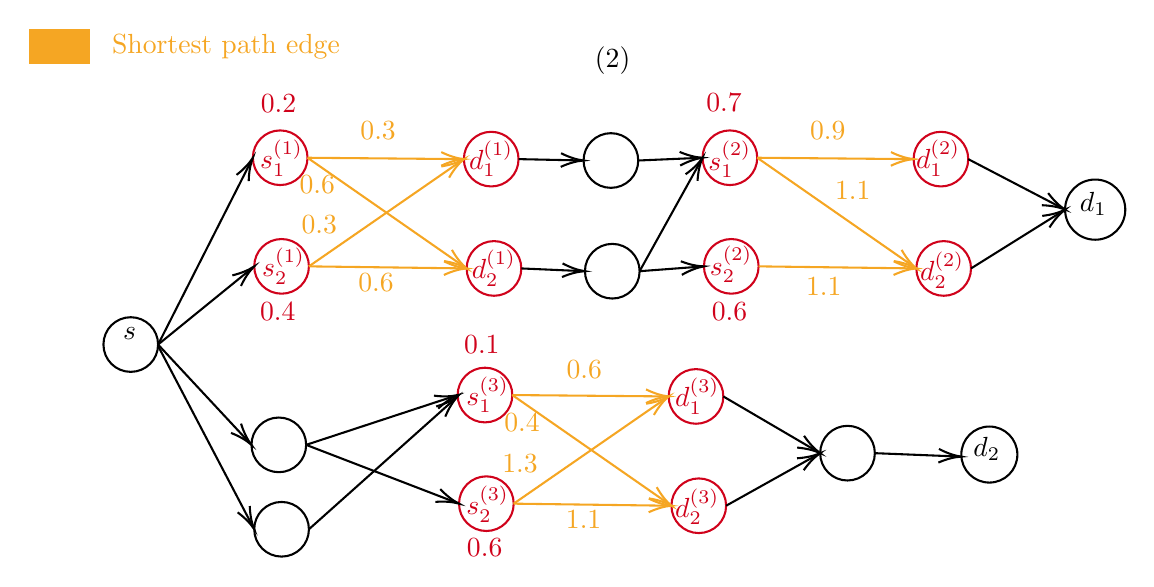
\begin{tikzpicture}[x=0.75pt,y=0.75pt,yscale=-1,xscale=1]
%uncomment if require: \path (0,285); %set diagram left start at 0, and has height of 285

%Shape: Circle [id:dp18617235606011406] 
\draw   (101.67,164.17) .. controls (101.67,156.89) and (107.56,151) .. (114.83,151) .. controls (122.11,151) and (128,156.89) .. (128,164.17) .. controls (128,171.44) and (122.11,177.33) .. (114.83,177.33) .. controls (107.56,177.33) and (101.67,171.44) .. (101.67,164.17) -- cycle ;
%Shape: Circle [id:dp3564338123926274] 
\draw   (565,99.17) .. controls (565,91.16) and (571.49,84.67) .. (579.5,84.67) .. controls (587.51,84.67) and (594,91.16) .. (594,99.17) .. controls (594,107.17) and (587.51,113.67) .. (579.5,113.67) .. controls (571.49,113.67) and (565,107.17) .. (565,99.17) -- cycle ;
%Shape: Circle [id:dp46477341764805047] 
\draw   (515,217.17) .. controls (515,209.71) and (521.04,203.67) .. (528.5,203.67) .. controls (535.96,203.67) and (542,209.71) .. (542,217.17) .. controls (542,224.62) and (535.96,230.67) .. (528.5,230.67) .. controls (521.04,230.67) and (515,224.62) .. (515,217.17) -- cycle ;
%Shape: Circle [id:dp10316255300962207] 
\draw  [color={rgb, 255:red, 208; green, 2; blue, 27 }  ,draw opacity=1 ] (173.67,74.17) .. controls (173.67,66.89) and (179.56,61) .. (186.83,61) .. controls (194.11,61) and (200,66.89) .. (200,74.17) .. controls (200,81.44) and (194.11,87.33) .. (186.83,87.33) .. controls (179.56,87.33) and (173.67,81.44) .. (173.67,74.17) -- cycle ;
%Shape: Circle [id:dp6838274912968219] 
\draw  [color={rgb, 255:red, 208; green, 2; blue, 27 }  ,draw opacity=1 ] (275.33,74.83) .. controls (275.33,67.56) and (281.23,61.67) .. (288.5,61.67) .. controls (295.77,61.67) and (301.67,67.56) .. (301.67,74.83) .. controls (301.67,82.11) and (295.77,88) .. (288.5,88) .. controls (281.23,88) and (275.33,82.11) .. (275.33,74.83) -- cycle ;
%Shape: Circle [id:dp0015477784958768392] 
\draw  [color={rgb, 255:red, 208; green, 2; blue, 27 }  ,draw opacity=1 ] (174.33,126.5) .. controls (174.33,119.23) and (180.23,113.33) .. (187.5,113.33) .. controls (194.77,113.33) and (200.67,119.23) .. (200.67,126.5) .. controls (200.67,133.77) and (194.77,139.67) .. (187.5,139.67) .. controls (180.23,139.67) and (174.33,133.77) .. (174.33,126.5) -- cycle ;
%Shape: Circle [id:dp1687195917390647] 
\draw  [color={rgb, 255:red, 208; green, 2; blue, 27 }  ,draw opacity=1 ] (276.67,127.5) .. controls (276.67,120.23) and (282.56,114.33) .. (289.83,114.33) .. controls (297.11,114.33) and (303,120.23) .. (303,127.5) .. controls (303,134.77) and (297.11,140.67) .. (289.83,140.67) .. controls (282.56,140.67) and (276.67,134.77) .. (276.67,127.5) -- cycle ;
%Shape: Circle [id:dp9552420228118483] 
\draw  [color={rgb, 255:red, 208; green, 2; blue, 27 }  ,draw opacity=1 ] (390.33,74.17) .. controls (390.33,66.89) and (396.23,61) .. (403.5,61) .. controls (410.77,61) and (416.67,66.89) .. (416.67,74.17) .. controls (416.67,81.44) and (410.77,87.33) .. (403.5,87.33) .. controls (396.23,87.33) and (390.33,81.44) .. (390.33,74.17) -- cycle ;
%Shape: Circle [id:dp25889654363877246] 
\draw  [color={rgb, 255:red, 208; green, 2; blue, 27 }  ,draw opacity=1 ] (492,74.83) .. controls (492,67.56) and (497.89,61.67) .. (505.17,61.67) .. controls (512.44,61.67) and (518.33,67.56) .. (518.33,74.83) .. controls (518.33,82.11) and (512.44,88) .. (505.17,88) .. controls (497.89,88) and (492,82.11) .. (492,74.83) -- cycle ;
%Shape: Circle [id:dp6909207134408744] 
\draw  [color={rgb, 255:red, 208; green, 2; blue, 27 }  ,draw opacity=1 ] (391,126.5) .. controls (391,119.23) and (396.89,113.33) .. (404.17,113.33) .. controls (411.44,113.33) and (417.33,119.23) .. (417.33,126.5) .. controls (417.33,133.77) and (411.44,139.67) .. (404.17,139.67) .. controls (396.89,139.67) and (391,133.77) .. (391,126.5) -- cycle ;
%Shape: Circle [id:dp9760038906173942] 
\draw  [color={rgb, 255:red, 208; green, 2; blue, 27 }  ,draw opacity=1 ] (493.33,127.5) .. controls (493.33,120.23) and (499.23,114.33) .. (506.5,114.33) .. controls (513.77,114.33) and (519.67,120.23) .. (519.67,127.5) .. controls (519.67,134.77) and (513.77,140.67) .. (506.5,140.67) .. controls (499.23,140.67) and (493.33,134.77) .. (493.33,127.5) -- cycle ;
%Shape: Circle [id:dp6599402287005878] 
\draw  [color={rgb, 255:red, 208; green, 2; blue, 27 }  ,draw opacity=1 ] (272.33,188.5) .. controls (272.33,181.23) and (278.23,175.33) .. (285.5,175.33) .. controls (292.77,175.33) and (298.67,181.23) .. (298.67,188.5) .. controls (298.67,195.77) and (292.77,201.67) .. (285.5,201.67) .. controls (278.23,201.67) and (272.33,195.77) .. (272.33,188.5) -- cycle ;
%Shape: Circle [id:dp28748286920541477] 
\draw  [color={rgb, 255:red, 208; green, 2; blue, 27 }  ,draw opacity=1 ] (374,189.17) .. controls (374,181.89) and (379.89,176) .. (387.17,176) .. controls (394.44,176) and (400.33,181.89) .. (400.33,189.17) .. controls (400.33,196.44) and (394.44,202.33) .. (387.17,202.33) .. controls (379.89,202.33) and (374,196.44) .. (374,189.17) -- cycle ;
%Shape: Circle [id:dp46685976857726863] 
\draw  [color={rgb, 255:red, 208; green, 2; blue, 27 }  ,draw opacity=1 ] (273,240.83) .. controls (273,233.56) and (278.89,227.67) .. (286.17,227.67) .. controls (293.44,227.67) and (299.33,233.56) .. (299.33,240.83) .. controls (299.33,248.11) and (293.44,254) .. (286.17,254) .. controls (278.89,254) and (273,248.11) .. (273,240.83) -- cycle ;
%Shape: Circle [id:dp7122398057420234] 
\draw  [color={rgb, 255:red, 208; green, 2; blue, 27 }  ,draw opacity=1 ] (375.33,241.83) .. controls (375.33,234.56) and (381.23,228.67) .. (388.5,228.67) .. controls (395.77,228.67) and (401.67,234.56) .. (401.67,241.83) .. controls (401.67,249.11) and (395.77,255) .. (388.5,255) .. controls (381.23,255) and (375.33,249.11) .. (375.33,241.83) -- cycle ;
%Shape: Circle [id:dp5865947417809445] 
\draw   (173,212.5) .. controls (173,205.23) and (178.89,199.33) .. (186.17,199.33) .. controls (193.44,199.33) and (199.33,205.23) .. (199.33,212.5) .. controls (199.33,219.77) and (193.44,225.67) .. (186.17,225.67) .. controls (178.89,225.67) and (173,219.77) .. (173,212.5) -- cycle ;
%Shape: Circle [id:dp7671398986660478] 
\draw   (333.67,128.83) .. controls (333.67,121.56) and (339.56,115.67) .. (346.83,115.67) .. controls (354.11,115.67) and (360,121.56) .. (360,128.83) .. controls (360,136.11) and (354.11,142) .. (346.83,142) .. controls (339.56,142) and (333.67,136.11) .. (333.67,128.83) -- cycle ;
%Shape: Circle [id:dp34193229943159387] 
\draw   (333,75.5) .. controls (333,68.23) and (338.89,62.33) .. (346.17,62.33) .. controls (353.44,62.33) and (359.33,68.23) .. (359.33,75.5) .. controls (359.33,82.77) and (353.44,88.67) .. (346.17,88.67) .. controls (338.89,88.67) and (333,82.77) .. (333,75.5) -- cycle ;
%Shape: Circle [id:dp9884144584126842] 
\draw   (447,216.5) .. controls (447,209.23) and (452.89,203.33) .. (460.17,203.33) .. controls (467.44,203.33) and (473.33,209.23) .. (473.33,216.5) .. controls (473.33,223.77) and (467.44,229.67) .. (460.17,229.67) .. controls (452.89,229.67) and (447,223.77) .. (447,216.5) -- cycle ;
%Straight Lines [id:da6877552394593465] 
\draw    (128,164.17) -- (172.76,75.95) ;
\draw [shift={(173.67,74.17)}, rotate = 116.9] [color={rgb, 255:red, 0; green, 0; blue, 0 }  ][line width=0.75]    (10.93,-3.29) .. controls (6.95,-1.4) and (3.31,-0.3) .. (0,0) .. controls (3.31,0.3) and (6.95,1.4) .. (10.93,3.29)   ;
%Straight Lines [id:da394752640318331] 
\draw    (128,164.17) -- (172.78,127.76) ;
\draw [shift={(174.33,126.5)}, rotate = 140.89] [color={rgb, 255:red, 0; green, 0; blue, 0 }  ][line width=0.75]    (10.93,-3.29) .. controls (6.95,-1.4) and (3.31,-0.3) .. (0,0) .. controls (3.31,0.3) and (6.95,1.4) .. (10.93,3.29)   ;
%Straight Lines [id:da15258693046369176] 
\draw    (301.67,74.83) -- (331,75.46) ;
\draw [shift={(333,75.5)}, rotate = 181.22] [color={rgb, 255:red, 0; green, 0; blue, 0 }  ][line width=0.75]    (10.93,-3.29) .. controls (6.95,-1.4) and (3.31,-0.3) .. (0,0) .. controls (3.31,0.3) and (6.95,1.4) .. (10.93,3.29)   ;
%Straight Lines [id:da782352869531761] 
\draw    (359.33,75.5) -- (388.34,74.25) ;
\draw [shift={(390.33,74.17)}, rotate = 177.54] [color={rgb, 255:red, 0; green, 0; blue, 0 }  ][line width=0.75]    (10.93,-3.29) .. controls (6.95,-1.4) and (3.31,-0.3) .. (0,0) .. controls (3.31,0.3) and (6.95,1.4) .. (10.93,3.29)   ;
%Straight Lines [id:da34544714873645455] 
\draw    (360,128.83) -- (389.01,126.65) ;
\draw [shift={(391,126.5)}, rotate = 175.7] [color={rgb, 255:red, 0; green, 0; blue, 0 }  ][line width=0.75]    (10.93,-3.29) .. controls (6.95,-1.4) and (3.31,-0.3) .. (0,0) .. controls (3.31,0.3) and (6.95,1.4) .. (10.93,3.29)   ;
%Straight Lines [id:da009592243622288832] 
\draw    (303,127.5) -- (331.67,128.75) ;
\draw [shift={(333.67,128.83)}, rotate = 182.49] [color={rgb, 255:red, 0; green, 0; blue, 0 }  ][line width=0.75]    (10.93,-3.29) .. controls (6.95,-1.4) and (3.31,-0.3) .. (0,0) .. controls (3.31,0.3) and (6.95,1.4) .. (10.93,3.29)   ;
%Straight Lines [id:da5936394696536158] 
\draw    (360,128.83) -- (389.36,75.92) ;
\draw [shift={(390.33,74.17)}, rotate = 119.02] [color={rgb, 255:red, 0; green, 0; blue, 0 }  ][line width=0.75]    (10.93,-3.29) .. controls (6.95,-1.4) and (3.31,-0.3) .. (0,0) .. controls (3.31,0.3) and (6.95,1.4) .. (10.93,3.29)   ;
%Straight Lines [id:da9405482287037086] 
\draw    (128,164.17) -- (171.64,211.04) ;
\draw [shift={(173,212.5)}, rotate = 227.05] [color={rgb, 255:red, 0; green, 0; blue, 0 }  ][line width=0.75]    (10.93,-3.29) .. controls (6.95,-1.4) and (3.31,-0.3) .. (0,0) .. controls (3.31,0.3) and (6.95,1.4) .. (10.93,3.29)   ;
%Straight Lines [id:da15883497129538005] 
\draw    (199.33,212.5) -- (270.43,189.12) ;
\draw [shift={(272.33,188.5)}, rotate = 161.8] [color={rgb, 255:red, 0; green, 0; blue, 0 }  ][line width=0.75]    (10.93,-3.29) .. controls (6.95,-1.4) and (3.31,-0.3) .. (0,0) .. controls (3.31,0.3) and (6.95,1.4) .. (10.93,3.29)   ;
%Straight Lines [id:da023929937885482477] 
\draw    (199.33,212.5) -- (271.13,240.12) ;
\draw [shift={(273,240.83)}, rotate = 201.04] [color={rgb, 255:red, 0; green, 0; blue, 0 }  ][line width=0.75]    (10.93,-3.29) .. controls (6.95,-1.4) and (3.31,-0.3) .. (0,0) .. controls (3.31,0.3) and (6.95,1.4) .. (10.93,3.29)   ;
%Straight Lines [id:da3061171028903873] 
\draw    (400.33,189.17) -- (445.27,215.49) ;
\draw [shift={(447,216.5)}, rotate = 210.36] [color={rgb, 255:red, 0; green, 0; blue, 0 }  ][line width=0.75]    (10.93,-3.29) .. controls (6.95,-1.4) and (3.31,-0.3) .. (0,0) .. controls (3.31,0.3) and (6.95,1.4) .. (10.93,3.29)   ;
%Straight Lines [id:da3614690401389955] 
\draw    (518.33,74.83) -- (563.23,98.24) ;
\draw [shift={(565,99.17)}, rotate = 207.54] [color={rgb, 255:red, 0; green, 0; blue, 0 }  ][line width=0.75]    (10.93,-3.29) .. controls (6.95,-1.4) and (3.31,-0.3) .. (0,0) .. controls (3.31,0.3) and (6.95,1.4) .. (10.93,3.29)   ;
%Straight Lines [id:da3184299782445028] 
\draw    (519.67,127.5) -- (563.3,100.23) ;
\draw [shift={(565,99.17)}, rotate = 147.99] [color={rgb, 255:red, 0; green, 0; blue, 0 }  ][line width=0.75]    (10.93,-3.29) .. controls (6.95,-1.4) and (3.31,-0.3) .. (0,0) .. controls (3.31,0.3) and (6.95,1.4) .. (10.93,3.29)   ;
%Straight Lines [id:da5710531022579275] 
\draw    (401.67,241.83) -- (445.25,217.48) ;
\draw [shift={(447,216.5)}, rotate = 150.8] [color={rgb, 255:red, 0; green, 0; blue, 0 }  ][line width=0.75]    (10.93,-3.29) .. controls (6.95,-1.4) and (3.31,-0.3) .. (0,0) .. controls (3.31,0.3) and (6.95,1.4) .. (10.93,3.29)   ;
%Straight Lines [id:da7076529816785542] 
\draw    (473.33,216.5) -- (513,218.09) ;
\draw [shift={(515,218.17)}, rotate = 182.29] [color={rgb, 255:red, 0; green, 0; blue, 0 }  ][line width=0.75]    (10.93,-3.29) .. controls (6.95,-1.4) and (3.31,-0.3) .. (0,0) .. controls (3.31,0.3) and (6.95,1.4) .. (10.93,3.29)   ;
%Straight Lines [id:da4056364599672331] 
\draw [color={rgb, 255:red, 245; green, 166; blue, 35 }  ,draw opacity=1 ]   (200,74.17) -- (273.33,74.82) ;
\draw [shift={(275.33,74.83)}, rotate = 180.51] [color={rgb, 255:red, 245; green, 166; blue, 35 }  ,draw opacity=1 ][line width=0.75]    (10.93,-3.29) .. controls (6.95,-1.4) and (3.31,-0.3) .. (0,0) .. controls (3.31,0.3) and (6.95,1.4) .. (10.93,3.29)   ;
%Straight Lines [id:da5323409264535977] 
\draw [color={rgb, 255:red, 245; green, 166; blue, 35 }  ,draw opacity=1 ]   (200,74.17) -- (275.02,126.36) ;
\draw [shift={(276.67,127.5)}, rotate = 214.82] [color={rgb, 255:red, 245; green, 166; blue, 35 }  ,draw opacity=1 ][line width=0.75]    (10.93,-3.29) .. controls (6.95,-1.4) and (3.31,-0.3) .. (0,0) .. controls (3.31,0.3) and (6.95,1.4) .. (10.93,3.29)   ;
%Straight Lines [id:da6190466219142452] 
\draw [color={rgb, 255:red, 245; green, 166; blue, 35 }  ,draw opacity=1 ]   (200.67,126.5) -- (273.69,75.97) ;
\draw [shift={(275.33,74.83)}, rotate = 145.32] [color={rgb, 255:red, 245; green, 166; blue, 35 }  ,draw opacity=1 ][line width=0.75]    (10.93,-3.29) .. controls (6.95,-1.4) and (3.31,-0.3) .. (0,0) .. controls (3.31,0.3) and (6.95,1.4) .. (10.93,3.29)   ;
%Straight Lines [id:da2651474875712534] 
\draw [color={rgb, 255:red, 245; green, 166; blue, 35 }  ,draw opacity=1 ]   (200.67,126.5) -- (274.67,127.47) ;
\draw [shift={(276.67,127.5)}, rotate = 180.75] [color={rgb, 255:red, 245; green, 166; blue, 35 }  ,draw opacity=1 ][line width=0.75]    (10.93,-3.29) .. controls (6.95,-1.4) and (3.31,-0.3) .. (0,0) .. controls (3.31,0.3) and (6.95,1.4) .. (10.93,3.29)   ;
%Straight Lines [id:da13831698845332174] 
\draw [color={rgb, 255:red, 245; green, 166; blue, 35 }  ,draw opacity=1 ]   (417.33,126.5) -- (491.33,127.47) ;
\draw [shift={(493.33,127.5)}, rotate = 180.75] [color={rgb, 255:red, 245; green, 166; blue, 35 }  ,draw opacity=1 ][line width=0.75]    (10.93,-3.29) .. controls (6.95,-1.4) and (3.31,-0.3) .. (0,0) .. controls (3.31,0.3) and (6.95,1.4) .. (10.93,3.29)   ;
%Straight Lines [id:da21566859993293752] 
\draw [color={rgb, 255:red, 245; green, 166; blue, 35 }  ,draw opacity=1 ]   (416.67,74.17) -- (490,74.82) ;
\draw [shift={(492,74.83)}, rotate = 180.51] [color={rgb, 255:red, 245; green, 166; blue, 35 }  ,draw opacity=1 ][line width=0.75]    (10.93,-3.29) .. controls (6.95,-1.4) and (3.31,-0.3) .. (0,0) .. controls (3.31,0.3) and (6.95,1.4) .. (10.93,3.29)   ;
%Straight Lines [id:da16168036928385043] 
\draw [color={rgb, 255:red, 245; green, 166; blue, 35 }  ,draw opacity=1 ]   (416.67,74.17) -- (491.69,126.36) ;
\draw [shift={(493.33,127.5)}, rotate = 214.82] [color={rgb, 255:red, 245; green, 166; blue, 35 }  ,draw opacity=1 ][line width=0.75]    (10.93,-3.29) .. controls (6.95,-1.4) and (3.31,-0.3) .. (0,0) .. controls (3.31,0.3) and (6.95,1.4) .. (10.93,3.29)   ;
%Straight Lines [id:da16049661825614403] 
\draw [color={rgb, 255:red, 245; green, 166; blue, 35 }  ,draw opacity=1 ]   (299.33,240.83) -- (373.33,241.81) ;
\draw [shift={(375.33,241.83)}, rotate = 180.75] [color={rgb, 255:red, 245; green, 166; blue, 35 }  ,draw opacity=1 ][line width=0.75]    (10.93,-3.29) .. controls (6.95,-1.4) and (3.31,-0.3) .. (0,0) .. controls (3.31,0.3) and (6.95,1.4) .. (10.93,3.29)   ;
%Straight Lines [id:da8529718470925769] 
\draw [color={rgb, 255:red, 245; green, 166; blue, 35 }  ,draw opacity=1 ]   (299.33,240.83) -- (372.36,190.3) ;
\draw [shift={(374,189.17)}, rotate = 145.32] [color={rgb, 255:red, 245; green, 166; blue, 35 }  ,draw opacity=1 ][line width=0.75]    (10.93,-3.29) .. controls (6.95,-1.4) and (3.31,-0.3) .. (0,0) .. controls (3.31,0.3) and (6.95,1.4) .. (10.93,3.29)   ;
%Straight Lines [id:da7266995040000397] 
\draw [color={rgb, 255:red, 245; green, 166; blue, 35 }  ,draw opacity=1 ]   (298.67,188.5) -- (373.69,240.69) ;
\draw [shift={(375.33,241.83)}, rotate = 214.82] [color={rgb, 255:red, 245; green, 166; blue, 35 }  ,draw opacity=1 ][line width=0.75]    (10.93,-3.29) .. controls (6.95,-1.4) and (3.31,-0.3) .. (0,0) .. controls (3.31,0.3) and (6.95,1.4) .. (10.93,3.29)   ;
%Straight Lines [id:da41872323090118213] 
\draw [color={rgb, 255:red, 245; green, 166; blue, 35 }  ,draw opacity=1 ]   (298.67,188.5) -- (372,189.15) ;
\draw [shift={(374,189.17)}, rotate = 180.51] [color={rgb, 255:red, 245; green, 166; blue, 35 }  ,draw opacity=1 ][line width=0.75]    (10.93,-3.29) .. controls (6.95,-1.4) and (3.31,-0.3) .. (0,0) .. controls (3.31,0.3) and (6.95,1.4) .. (10.93,3.29)   ;
%Shape: Rectangle [id:dp6916523427530652] 
\draw  [draw opacity=0][fill={rgb, 255:red, 245; green, 166; blue, 35 }  ,fill opacity=1 ] (65.67,12) -- (95.33,12) -- (95.33,29) -- (65.67,29) -- cycle ;
%Shape: Circle [id:dp2498458502029317] 
\draw   (174.33,253.17) .. controls (174.33,245.89) and (180.23,240) .. (187.5,240) .. controls (194.77,240) and (200.67,245.89) .. (200.67,253.17) .. controls (200.67,260.44) and (194.77,266.33) .. (187.5,266.33) .. controls (180.23,266.33) and (174.33,260.44) .. (174.33,253.17) -- cycle ;
%Straight Lines [id:da2990184735571968] 
\draw    (128,164.83) -- (173.4,251.4) ;
\draw [shift={(174.33,253.17)}, rotate = 242.32] [color={rgb, 255:red, 0; green, 0; blue, 0 }  ][line width=0.75]    (10.93,-3.29) .. controls (6.95,-1.4) and (3.31,-0.3) .. (0,0) .. controls (3.31,0.3) and (6.95,1.4) .. (10.93,3.29)   ;
%Straight Lines [id:da8905517535796914] 
\draw    (200.67,253.17) -- (270.84,190.5) ;
\draw [shift={(272.33,189.17)}, rotate = 138.23] [color={rgb, 255:red, 0; green, 0; blue, 0 }  ][line width=0.75]    (10.93,-3.29) .. controls (6.95,-1.4) and (3.31,-0.3) .. (0,0) .. controls (3.31,0.3) and (6.95,1.4) .. (10.93,3.29)   ;

% Text Node
\draw (175.67,64.07) node [anchor=north west][inner sep=0.75pt]  [color={rgb, 255:red, 208; green, 2; blue, 27 }  ,opacity=1 ]  {$s_{1}^{( 1)}$};
% Text Node
\draw (176.67,116.07) node [anchor=north west][inner sep=0.75pt]  [color={rgb, 255:red, 208; green, 2; blue, 27 }  ,opacity=1 ]  {$s_{2}^{( 1)}$};
% Text Node
\draw (277.67,117.07) node [anchor=north west][inner sep=0.75pt]  [color={rgb, 255:red, 208; green, 2; blue, 27 }  ,opacity=1 ]  {$d_{2}^{( 1)}$};
% Text Node
\draw (276.33,64.4) node [anchor=north west][inner sep=0.75pt]  [color={rgb, 255:red, 208; green, 2; blue, 27 }  ,opacity=1 ]  {$d_{1}^{( 1)}$};
% Text Node
\draw (275,178.07) node [anchor=north west][inner sep=0.75pt]  [color={rgb, 255:red, 208; green, 2; blue, 27 }  ,opacity=1 ]  {$s_{1}^{( 3)}$};
% Text Node
\draw (275,230.73) node [anchor=north west][inner sep=0.75pt]  [color={rgb, 255:red, 208; green, 2; blue, 27 }  ,opacity=1 ]  {$s_{2}^{( 3)}$};
% Text Node
\draw (375.67,178.73) node [anchor=north west][inner sep=0.75pt]  [color={rgb, 255:red, 208; green, 2; blue, 27 }  ,opacity=1 ]  {$d_{1}^{( 3)}$};
% Text Node
\draw (375.67,232.07) node [anchor=north west][inner sep=0.75pt]  [color={rgb, 255:red, 208; green, 2; blue, 27 }  ,opacity=1 ]  {$d_{2}^{( 3)}$};
% Text Node
\draw (491.67,64.07) node [anchor=north west][inner sep=0.75pt]  [color={rgb, 255:red, 208; green, 2; blue, 27 }  ,opacity=1 ]  {$d_{1}^{( 2)}$};
% Text Node
\draw (493.67,118.07) node [anchor=north west][inner sep=0.75pt]  [color={rgb, 255:red, 208; green, 2; blue, 27 }  ,opacity=1 ]  {$d_{2}^{( 2)}$};
% Text Node
\draw (391.67,64.73) node [anchor=north west][inner sep=0.75pt]  [color={rgb, 255:red, 208; green, 2; blue, 27 }  ,opacity=1 ]  {$s_{1}^{( 2)}$};
% Text Node
\draw (392.33,115.4) node [anchor=north west][inner sep=0.75pt]  [color={rgb, 255:red, 208; green, 2; blue, 27 }  ,opacity=1 ]  {$s_{2}^{( 2)}$};
% Text Node
\draw (104.33,13) node [anchor=north west][inner sep=0.75pt]  [color={rgb, 255:red, 245; green, 166; blue, 35 }  ,opacity=1 ] [align=left] {Shortest path edge};
% Text Node
\draw (109.67,154.4) node [anchor=north west][inner sep=0.75pt]    {$s$};
% Text Node
\draw (570.67,89.4) node [anchor=north west][inner sep=0.75pt]    {$d_{1}$};
% Text Node
\draw (519.33,207.4) node [anchor=north west][inner sep=0.75pt]    {$d_{2}$};
% Text Node
\draw (176,42.4) node [anchor=north west][inner sep=0.75pt]  [color={rgb, 255:red, 208; green, 2; blue, 27 }  ,opacity=1 ]  {$0.2$};
% Text Node
\draw (175.67,142.73) node [anchor=north west][inner sep=0.75pt]  [color={rgb, 255:red, 208; green, 2; blue, 27 }  ,opacity=1 ]  {$0.4$};
% Text Node
\draw (224,55.4) node [anchor=north west][inner sep=0.75pt]  [color={rgb, 255:red, 245; green, 166; blue, 35 }  ,opacity=1 ]  {$0.3$};
% Text Node
\draw (194.67,81.4) node [anchor=north west][inner sep=0.75pt]  [color={rgb, 255:red, 245; green, 166; blue, 35 }  ,opacity=1 ]  {$0.6$};
% Text Node
\draw (223,128.4) node [anchor=north west][inner sep=0.75pt]  [color={rgb, 255:red, 245; green, 166; blue, 35 }  ,opacity=1 ]  {$0.6$};
% Text Node
\draw (195.67,100.73) node [anchor=north west][inner sep=0.75pt]  [color={rgb, 255:red, 245; green, 166; blue, 35 }  ,opacity=1 ]  {$0.3$};
% Text Node
\draw (440.67,55.07) node [anchor=north west][inner sep=0.75pt]  [color={rgb, 255:red, 245; green, 166; blue, 35 }  ,opacity=1 ]  {$0.9$};
% Text Node
\draw (452.67,84.4) node [anchor=north west][inner sep=0.75pt]  [color={rgb, 255:red, 245; green, 166; blue, 35 }  ,opacity=1 ]  {$1.1$};
% Text Node
\draw (438.67,130.4) node [anchor=north west][inner sep=0.75pt]  [color={rgb, 255:red, 245; green, 166; blue, 35 }  ,opacity=1 ]  {$1.1$};
% Text Node
\draw (390.67,41.73) node [anchor=north west][inner sep=0.75pt]  [color={rgb, 255:red, 208; green, 2; blue, 27 }  ,opacity=1 ]  {$0.7$};
% Text Node
\draw (393.33,142.4) node [anchor=north west][inner sep=0.75pt]  [color={rgb, 255:red, 208; green, 2; blue, 27 }  ,opacity=1 ]  {$0.6$};
% Text Node
\draw (274,158.4) node [anchor=north west][inner sep=0.75pt]  [color={rgb, 255:red, 208; green, 2; blue, 27 }  ,opacity=1 ]  {$0.1$};
% Text Node
\draw (275.33,256.4) node [anchor=north west][inner sep=0.75pt]  [color={rgb, 255:red, 208; green, 2; blue, 27 }  ,opacity=1 ]  {$0.6$};
% Text Node
\draw (323.33,170.4) node [anchor=north west][inner sep=0.75pt]  [color={rgb, 255:red, 245; green, 166; blue, 35 }  ,opacity=1 ]  {$0.6$};
% Text Node
\draw (323,242.73) node [anchor=north west][inner sep=0.75pt]  [color={rgb, 255:red, 245; green, 166; blue, 35 }  ,opacity=1 ]  {$1.1$};
% Text Node
\draw (293.33,195.73) node [anchor=north west][inner sep=0.75pt]  [color={rgb, 255:red, 245; green, 166; blue, 35 }  ,opacity=1 ]  {$0.4$};
% Text Node
\draw (292.33,215.73) node [anchor=north west][inner sep=0.75pt]  [color={rgb, 255:red, 245; green, 166; blue, 35 }  ,opacity=1 ]  {$1.3$};
% Text Node
\draw (337,19.33) node [anchor=north west][inner sep=0.75pt]   [align=left] {(2)};


\end{tikzpicture}



\tikzset{every picture/.style={line width=0.75pt}} %set default line width to 0.75pt        

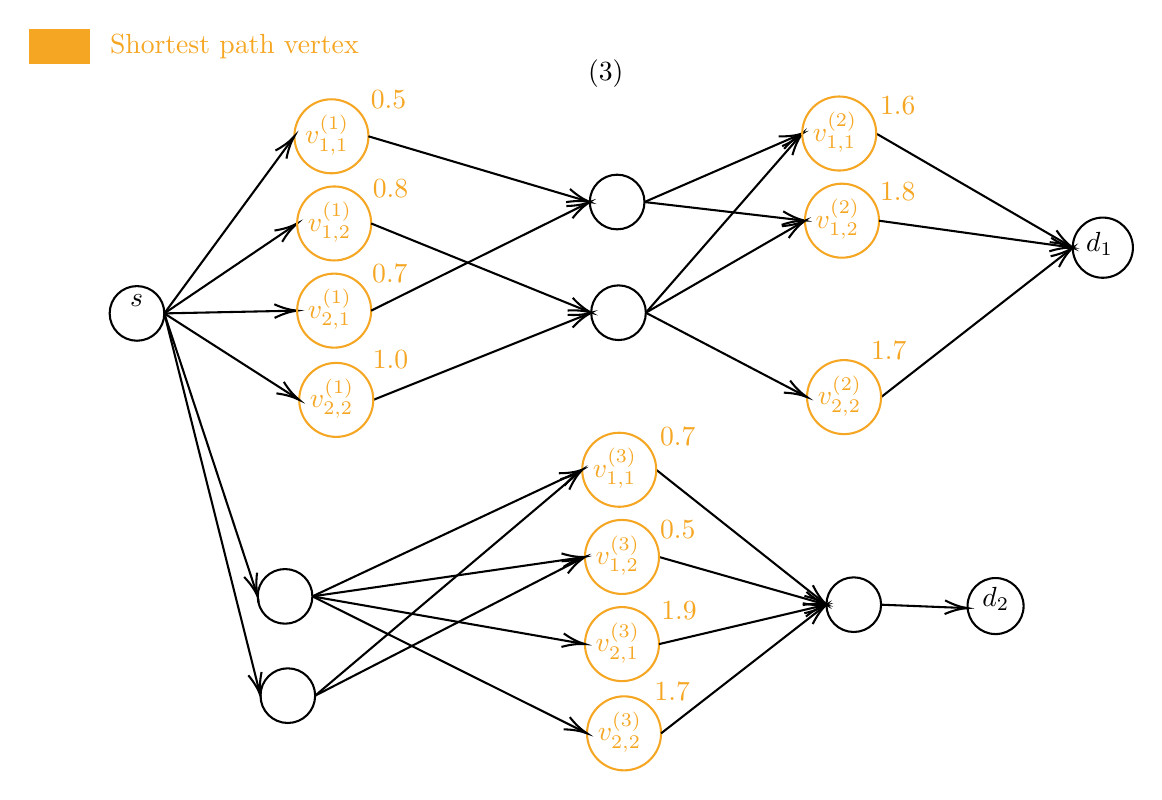
\begin{tikzpicture}[x=0.75pt,y=0.75pt,yscale=-1,xscale=1]
%uncomment if require: \path (0,392); %set diagram left start at 0, and has height of 392

%Shape: Circle [id:dp17851147211027696] 
\draw   (100,151.03) .. controls (100,143.76) and (105.89,137.87) .. (113.17,137.87) .. controls (120.44,137.87) and (126.33,143.76) .. (126.33,151.03) .. controls (126.33,158.31) and (120.44,164.2) .. (113.17,164.2) .. controls (105.89,164.2) and (100,158.31) .. (100,151.03) -- cycle ;
%Shape: Circle [id:dp9017901743964531] 
\draw   (564,119.37) .. controls (564,111.36) and (570.49,104.87) .. (578.5,104.87) .. controls (586.51,104.87) and (593,111.36) .. (593,119.37) .. controls (593,127.37) and (586.51,133.87) .. (578.5,133.87) .. controls (570.49,133.87) and (564,127.37) .. (564,119.37) -- cycle ;
%Shape: Circle [id:dp38157590235600347] 
\draw   (513.33,292.03) .. controls (513.33,284.58) and (519.38,278.53) .. (526.83,278.53) .. controls (534.29,278.53) and (540.33,284.58) .. (540.33,292.03) .. controls (540.33,299.49) and (534.29,305.53) .. (526.83,305.53) .. controls (519.38,305.53) and (513.33,299.49) .. (513.33,292.03) -- cycle ;
%Shape: Circle [id:dp6983459245889354] 
\draw  [color={rgb, 255:red, 245; green, 166; blue, 35 }  ,draw opacity=1 ] (189,65.7) .. controls (189,55.85) and (196.98,47.87) .. (206.83,47.87) .. controls (216.68,47.87) and (224.67,55.85) .. (224.67,65.7) .. controls (224.67,75.55) and (216.68,83.53) .. (206.83,83.53) .. controls (196.98,83.53) and (189,75.55) .. (189,65.7) -- cycle ;
%Shape: Circle [id:dp41356894127960553] 
\draw   (171.33,287.37) .. controls (171.33,280.09) and (177.23,274.2) .. (184.5,274.2) .. controls (191.77,274.2) and (197.67,280.09) .. (197.67,287.37) .. controls (197.67,294.64) and (191.77,300.53) .. (184.5,300.53) .. controls (177.23,300.53) and (171.33,294.64) .. (171.33,287.37) -- cycle ;
%Shape: Circle [id:dp08333811829768267] 
\draw   (332,150.7) .. controls (332,143.43) and (337.89,137.53) .. (345.17,137.53) .. controls (352.44,137.53) and (358.33,143.43) .. (358.33,150.7) .. controls (358.33,157.97) and (352.44,163.87) .. (345.17,163.87) .. controls (337.89,163.87) and (332,157.97) .. (332,150.7) -- cycle ;
%Shape: Circle [id:dp1467622933415249] 
\draw   (331.33,97.37) .. controls (331.33,90.09) and (337.23,84.2) .. (344.5,84.2) .. controls (351.77,84.2) and (357.67,90.09) .. (357.67,97.37) .. controls (357.67,104.64) and (351.77,110.53) .. (344.5,110.53) .. controls (337.23,110.53) and (331.33,104.64) .. (331.33,97.37) -- cycle ;
%Shape: Circle [id:dp996508933539636] 
\draw   (445.33,291.37) .. controls (445.33,284.09) and (451.23,278.2) .. (458.5,278.2) .. controls (465.77,278.2) and (471.67,284.09) .. (471.67,291.37) .. controls (471.67,298.64) and (465.77,304.53) .. (458.5,304.53) .. controls (451.23,304.53) and (445.33,298.64) .. (445.33,291.37) -- cycle ;
%Straight Lines [id:da08986148868331001] 
\draw    (126.33,151.03) -- (187.82,67.31) ;
\draw [shift={(189,65.7)}, rotate = 126.29] [color={rgb, 255:red, 0; green, 0; blue, 0 }  ][line width=0.75]    (10.93,-3.29) .. controls (6.95,-1.4) and (3.31,-0.3) .. (0,0) .. controls (3.31,0.3) and (6.95,1.4) .. (10.93,3.29)   ;
%Straight Lines [id:da4653162504630415] 
\draw    (126.33,151.03) -- (188.68,108.82) ;
\draw [shift={(190.33,107.7)}, rotate = 145.9] [color={rgb, 255:red, 0; green, 0; blue, 0 }  ][line width=0.75]    (10.93,-3.29) .. controls (6.95,-1.4) and (3.31,-0.3) .. (0,0) .. controls (3.31,0.3) and (6.95,1.4) .. (10.93,3.29)   ;
%Straight Lines [id:da8227427836985428] 
\draw    (224.67,65.7) -- (329.42,96.8) ;
\draw [shift={(331.33,97.37)}, rotate = 196.53] [color={rgb, 255:red, 0; green, 0; blue, 0 }  ][line width=0.75]    (10.93,-3.29) .. controls (6.95,-1.4) and (3.31,-0.3) .. (0,0) .. controls (3.31,0.3) and (6.95,1.4) .. (10.93,3.29)   ;
%Straight Lines [id:da24898667365135618] 
\draw    (357.67,97.37) -- (431.83,65.16) ;
\draw [shift={(433.67,64.37)}, rotate = 156.53] [color={rgb, 255:red, 0; green, 0; blue, 0 }  ][line width=0.75]    (10.93,-3.29) .. controls (6.95,-1.4) and (3.31,-0.3) .. (0,0) .. controls (3.31,0.3) and (6.95,1.4) .. (10.93,3.29)   ;
%Straight Lines [id:da14684638786477922] 
\draw    (358.33,150.7) -- (432.35,65.87) ;
\draw [shift={(433.67,64.37)}, rotate = 131.11] [color={rgb, 255:red, 0; green, 0; blue, 0 }  ][line width=0.75]    (10.93,-3.29) .. controls (6.95,-1.4) and (3.31,-0.3) .. (0,0) .. controls (3.31,0.3) and (6.95,1.4) .. (10.93,3.29)   ;
%Straight Lines [id:da06872273038234522] 
\draw    (227,192.7) -- (330.14,151.44) ;
\draw [shift={(332,150.7)}, rotate = 158.2] [color={rgb, 255:red, 0; green, 0; blue, 0 }  ][line width=0.75]    (10.93,-3.29) .. controls (6.95,-1.4) and (3.31,-0.3) .. (0,0) .. controls (3.31,0.3) and (6.95,1.4) .. (10.93,3.29)   ;
%Straight Lines [id:da772305005094867] 
\draw    (357.67,97.37) -- (433.01,106.14) ;
\draw [shift={(435,106.37)}, rotate = 186.64] [color={rgb, 255:red, 0; green, 0; blue, 0 }  ][line width=0.75]    (10.93,-3.29) .. controls (6.95,-1.4) and (3.31,-0.3) .. (0,0) .. controls (3.31,0.3) and (6.95,1.4) .. (10.93,3.29)   ;
%Straight Lines [id:da18667936134495822] 
\draw    (126.33,151.03) -- (188.33,149.74) ;
\draw [shift={(190.33,149.7)}, rotate = 178.81] [color={rgb, 255:red, 0; green, 0; blue, 0 }  ][line width=0.75]    (10.93,-3.29) .. controls (6.95,-1.4) and (3.31,-0.3) .. (0,0) .. controls (3.31,0.3) and (6.95,1.4) .. (10.93,3.29)   ;
%Straight Lines [id:da20852599997022447] 
\draw    (197.67,287.37) -- (325.86,227.22) ;
\draw [shift={(327.67,226.37)}, rotate = 154.86] [color={rgb, 255:red, 0; green, 0; blue, 0 }  ][line width=0.75]    (10.93,-3.29) .. controls (6.95,-1.4) and (3.31,-0.3) .. (0,0) .. controls (3.31,0.3) and (6.95,1.4) .. (10.93,3.29)   ;
%Straight Lines [id:da738335568298228] 
\draw    (197.67,287.37) -- (327.02,268.65) ;
\draw [shift={(329,268.37)}, rotate = 171.77] [color={rgb, 255:red, 0; green, 0; blue, 0 }  ][line width=0.75]    (10.93,-3.29) .. controls (6.95,-1.4) and (3.31,-0.3) .. (0,0) .. controls (3.31,0.3) and (6.95,1.4) .. (10.93,3.29)   ;
%Straight Lines [id:da5514261747166165] 
\draw    (363.33,226.37) -- (443.77,290.12) ;
\draw [shift={(445.33,291.37)}, rotate = 218.4] [color={rgb, 255:red, 0; green, 0; blue, 0 }  ][line width=0.75]    (10.93,-3.29) .. controls (6.95,-1.4) and (3.31,-0.3) .. (0,0) .. controls (3.31,0.3) and (6.95,1.4) .. (10.93,3.29)   ;
%Straight Lines [id:da843917716358523] 
\draw    (469.33,64.37) -- (562.27,118.36) ;
\draw [shift={(564,119.37)}, rotate = 210.16] [color={rgb, 255:red, 0; green, 0; blue, 0 }  ][line width=0.75]    (10.93,-3.29) .. controls (6.95,-1.4) and (3.31,-0.3) .. (0,0) .. controls (3.31,0.3) and (6.95,1.4) .. (10.93,3.29)   ;
%Straight Lines [id:da5238652020863472] 
\draw    (471.67,191.37) -- (562.42,120.6) ;
\draw [shift={(564,119.37)}, rotate = 142.05] [color={rgb, 255:red, 0; green, 0; blue, 0 }  ][line width=0.75]    (10.93,-3.29) .. controls (6.95,-1.4) and (3.31,-0.3) .. (0,0) .. controls (3.31,0.3) and (6.95,1.4) .. (10.93,3.29)   ;
%Straight Lines [id:da17242007805439896] 
\draw    (364.67,268.37) -- (443.41,290.82) ;
\draw [shift={(445.33,291.37)}, rotate = 195.91] [color={rgb, 255:red, 0; green, 0; blue, 0 }  ][line width=0.75]    (10.93,-3.29) .. controls (6.95,-1.4) and (3.31,-0.3) .. (0,0) .. controls (3.31,0.3) and (6.95,1.4) .. (10.93,3.29)   ;
%Straight Lines [id:da3902426705919577] 
\draw    (471.67,291.37) -- (511.33,292.95) ;
\draw [shift={(513.33,293.03)}, rotate = 182.29] [color={rgb, 255:red, 0; green, 0; blue, 0 }  ][line width=0.75]    (10.93,-3.29) .. controls (6.95,-1.4) and (3.31,-0.3) .. (0,0) .. controls (3.31,0.3) and (6.95,1.4) .. (10.93,3.29)   ;
%Shape: Rectangle [id:dp6094611677122768] 
\draw  [draw opacity=0][fill={rgb, 255:red, 245; green, 166; blue, 35 }  ,fill opacity=1 ] (61,13.87) -- (90.67,13.87) -- (90.67,30.87) -- (61,30.87) -- cycle ;
%Shape: Circle [id:dp4669565597602978] 
\draw  [color={rgb, 255:red, 245; green, 166; blue, 35 }  ,draw opacity=1 ] (190.33,107.7) .. controls (190.33,97.85) and (198.32,89.87) .. (208.17,89.87) .. controls (218.02,89.87) and (226,97.85) .. (226,107.7) .. controls (226,117.55) and (218.02,125.53) .. (208.17,125.53) .. controls (198.32,125.53) and (190.33,117.55) .. (190.33,107.7) -- cycle ;
%Shape: Circle [id:dp4228842890834299] 
\draw  [color={rgb, 255:red, 245; green, 166; blue, 35 }  ,draw opacity=1 ] (190.33,149.7) .. controls (190.33,139.85) and (198.32,131.87) .. (208.17,131.87) .. controls (218.02,131.87) and (226,139.85) .. (226,149.7) .. controls (226,159.55) and (218.02,167.53) .. (208.17,167.53) .. controls (198.32,167.53) and (190.33,159.55) .. (190.33,149.7) -- cycle ;
%Shape: Circle [id:dp990547049026888] 
\draw  [color={rgb, 255:red, 245; green, 166; blue, 35 }  ,draw opacity=1 ] (191.33,192.7) .. controls (191.33,182.85) and (199.32,174.87) .. (209.17,174.87) .. controls (219.02,174.87) and (227,182.85) .. (227,192.7) .. controls (227,202.55) and (219.02,210.53) .. (209.17,210.53) .. controls (199.32,210.53) and (191.33,202.55) .. (191.33,192.7) -- cycle ;
%Straight Lines [id:da5328976035778661] 
\draw    (126.33,151.03) -- (189.65,191.62) ;
\draw [shift={(191.33,192.7)}, rotate = 212.66] [color={rgb, 255:red, 0; green, 0; blue, 0 }  ][line width=0.75]    (10.93,-3.29) .. controls (6.95,-1.4) and (3.31,-0.3) .. (0,0) .. controls (3.31,0.3) and (6.95,1.4) .. (10.93,3.29)   ;
%Straight Lines [id:da012840445484924468] 
\draw    (226,149.7) -- (329.54,98.26) ;
\draw [shift={(331.33,97.37)}, rotate = 153.58] [color={rgb, 255:red, 0; green, 0; blue, 0 }  ][line width=0.75]    (10.93,-3.29) .. controls (6.95,-1.4) and (3.31,-0.3) .. (0,0) .. controls (3.31,0.3) and (6.95,1.4) .. (10.93,3.29)   ;
%Straight Lines [id:da05022877826188399] 
\draw    (226,107.7) -- (330.15,149.95) ;
\draw [shift={(332,150.7)}, rotate = 202.08] [color={rgb, 255:red, 0; green, 0; blue, 0 }  ][line width=0.75]    (10.93,-3.29) .. controls (6.95,-1.4) and (3.31,-0.3) .. (0,0) .. controls (3.31,0.3) and (6.95,1.4) .. (10.93,3.29)   ;
%Shape: Circle [id:dp4893410740609936] 
\draw  [color={rgb, 255:red, 245; green, 166; blue, 35 }  ,draw opacity=1 ] (433.67,64.37) .. controls (433.67,54.52) and (441.65,46.53) .. (451.5,46.53) .. controls (461.35,46.53) and (469.33,54.52) .. (469.33,64.37) .. controls (469.33,74.22) and (461.35,82.2) .. (451.5,82.2) .. controls (441.65,82.2) and (433.67,74.22) .. (433.67,64.37) -- cycle ;
%Shape: Circle [id:dp677927715736903] 
\draw  [color={rgb, 255:red, 245; green, 166; blue, 35 }  ,draw opacity=1 ] (435,106.37) .. controls (435,96.52) and (442.98,88.53) .. (452.83,88.53) .. controls (462.68,88.53) and (470.67,96.52) .. (470.67,106.37) .. controls (470.67,116.22) and (462.68,124.2) .. (452.83,124.2) .. controls (442.98,124.2) and (435,116.22) .. (435,106.37) -- cycle ;
%Shape: Circle [id:dp5142660529514251] 
\draw  [color={rgb, 255:red, 245; green, 166; blue, 35 }  ,draw opacity=1 ] (436,191.37) .. controls (436,181.52) and (443.98,173.53) .. (453.83,173.53) .. controls (463.68,173.53) and (471.67,181.52) .. (471.67,191.37) .. controls (471.67,201.22) and (463.68,209.2) .. (453.83,209.2) .. controls (443.98,209.2) and (436,201.22) .. (436,191.37) -- cycle ;
%Straight Lines [id:da7976295808825846] 
\draw    (358.33,150.7) -- (433.27,107.37) ;
\draw [shift={(435,106.37)}, rotate = 149.96] [color={rgb, 255:red, 0; green, 0; blue, 0 }  ][line width=0.75]    (10.93,-3.29) .. controls (6.95,-1.4) and (3.31,-0.3) .. (0,0) .. controls (3.31,0.3) and (6.95,1.4) .. (10.93,3.29)   ;
%Straight Lines [id:da335511458316778] 
\draw    (358.33,150.7) -- (434.23,190.44) ;
\draw [shift={(436,191.37)}, rotate = 207.64] [color={rgb, 255:red, 0; green, 0; blue, 0 }  ][line width=0.75]    (10.93,-3.29) .. controls (6.95,-1.4) and (3.31,-0.3) .. (0,0) .. controls (3.31,0.3) and (6.95,1.4) .. (10.93,3.29)   ;
%Straight Lines [id:da10301810667861866] 
\draw    (470.67,106.37) -- (562.02,119.09) ;
\draw [shift={(564,119.37)}, rotate = 187.93] [color={rgb, 255:red, 0; green, 0; blue, 0 }  ][line width=0.75]    (10.93,-3.29) .. controls (6.95,-1.4) and (3.31,-0.3) .. (0,0) .. controls (3.31,0.3) and (6.95,1.4) .. (10.93,3.29)   ;
%Straight Lines [id:da12982170959122774] 
\draw    (126.33,151.03) -- (170.71,285.47) ;
\draw [shift={(171.33,287.37)}, rotate = 251.73] [color={rgb, 255:red, 0; green, 0; blue, 0 }  ][line width=0.75]    (10.93,-3.29) .. controls (6.95,-1.4) and (3.31,-0.3) .. (0,0) .. controls (3.31,0.3) and (6.95,1.4) .. (10.93,3.29)   ;
%Shape: Circle [id:dp981617420998659] 
\draw  [color={rgb, 255:red, 245; green, 166; blue, 35 }  ,draw opacity=1 ] (327.67,226.37) .. controls (327.67,216.52) and (335.65,208.53) .. (345.5,208.53) .. controls (355.35,208.53) and (363.33,216.52) .. (363.33,226.37) .. controls (363.33,236.22) and (355.35,244.2) .. (345.5,244.2) .. controls (335.65,244.2) and (327.67,236.22) .. (327.67,226.37) -- cycle ;
%Shape: Circle [id:dp09971639698750212] 
\draw  [color={rgb, 255:red, 245; green, 166; blue, 35 }  ,draw opacity=1 ] (329,268.37) .. controls (329,258.52) and (336.98,250.53) .. (346.83,250.53) .. controls (356.68,250.53) and (364.67,258.52) .. (364.67,268.37) .. controls (364.67,278.22) and (356.68,286.2) .. (346.83,286.2) .. controls (336.98,286.2) and (329,278.22) .. (329,268.37) -- cycle ;
%Shape: Circle [id:dp5551087171037332] 
\draw  [color={rgb, 255:red, 245; green, 166; blue, 35 }  ,draw opacity=1 ] (329,310.37) .. controls (329,300.52) and (336.98,292.53) .. (346.83,292.53) .. controls (356.68,292.53) and (364.67,300.52) .. (364.67,310.37) .. controls (364.67,320.22) and (356.68,328.2) .. (346.83,328.2) .. controls (336.98,328.2) and (329,320.22) .. (329,310.37) -- cycle ;
%Shape: Circle [id:dp15256818410563122] 
\draw  [color={rgb, 255:red, 245; green, 166; blue, 35 }  ,draw opacity=1 ] (330,353.37) .. controls (330,343.52) and (337.98,335.53) .. (347.83,335.53) .. controls (357.68,335.53) and (365.67,343.52) .. (365.67,353.37) .. controls (365.67,363.22) and (357.68,371.2) .. (347.83,371.2) .. controls (337.98,371.2) and (330,363.22) .. (330,353.37) -- cycle ;
%Straight Lines [id:da16501110939737074] 
\draw    (197.67,287.37) -- (327.03,310.02) ;
\draw [shift={(329,310.37)}, rotate = 189.93] [color={rgb, 255:red, 0; green, 0; blue, 0 }  ][line width=0.75]    (10.93,-3.29) .. controls (6.95,-1.4) and (3.31,-0.3) .. (0,0) .. controls (3.31,0.3) and (6.95,1.4) .. (10.93,3.29)   ;
%Straight Lines [id:da5240873746116668] 
\draw    (197.67,287.37) -- (328.21,352.47) ;
\draw [shift={(330,353.37)}, rotate = 206.51] [color={rgb, 255:red, 0; green, 0; blue, 0 }  ][line width=0.75]    (10.93,-3.29) .. controls (6.95,-1.4) and (3.31,-0.3) .. (0,0) .. controls (3.31,0.3) and (6.95,1.4) .. (10.93,3.29)   ;
%Straight Lines [id:da35953771328470796] 
\draw    (364.67,310.37) -- (443.39,291.83) ;
\draw [shift={(445.33,291.37)}, rotate = 166.75] [color={rgb, 255:red, 0; green, 0; blue, 0 }  ][line width=0.75]    (10.93,-3.29) .. controls (6.95,-1.4) and (3.31,-0.3) .. (0,0) .. controls (3.31,0.3) and (6.95,1.4) .. (10.93,3.29)   ;
%Straight Lines [id:da5189394201031894] 
\draw    (365.67,353.37) -- (443.75,292.6) ;
\draw [shift={(445.33,291.37)}, rotate = 142.11] [color={rgb, 255:red, 0; green, 0; blue, 0 }  ][line width=0.75]    (10.93,-3.29) .. controls (6.95,-1.4) and (3.31,-0.3) .. (0,0) .. controls (3.31,0.3) and (6.95,1.4) .. (10.93,3.29)   ;
%Shape: Circle [id:dp8203920176434067] 
\draw   (172.67,335.2) .. controls (172.67,327.93) and (178.56,322.03) .. (185.83,322.03) .. controls (193.11,322.03) and (199,327.93) .. (199,335.2) .. controls (199,342.47) and (193.11,348.37) .. (185.83,348.37) .. controls (178.56,348.37) and (172.67,342.47) .. (172.67,335.2) -- cycle ;
%Straight Lines [id:da6938944940906866] 
\draw    (126.33,151.03) -- (172.18,333.26) ;
\draw [shift={(172.67,335.2)}, rotate = 255.88] [color={rgb, 255:red, 0; green, 0; blue, 0 }  ][line width=0.75]    (10.93,-3.29) .. controls (6.95,-1.4) and (3.31,-0.3) .. (0,0) .. controls (3.31,0.3) and (6.95,1.4) .. (10.93,3.29)   ;
%Straight Lines [id:da4573975907370882] 
\draw    (199,335.2) -- (326.14,227.66) ;
\draw [shift={(327.67,226.37)}, rotate = 139.77] [color={rgb, 255:red, 0; green, 0; blue, 0 }  ][line width=0.75]    (10.93,-3.29) .. controls (6.95,-1.4) and (3.31,-0.3) .. (0,0) .. controls (3.31,0.3) and (6.95,1.4) .. (10.93,3.29)   ;
%Straight Lines [id:da26171440178000194] 
\draw    (199,335.2) -- (327.22,269.28) ;
\draw [shift={(329,268.37)}, rotate = 152.79] [color={rgb, 255:red, 0; green, 0; blue, 0 }  ][line width=0.75]    (10.93,-3.29) .. controls (6.95,-1.4) and (3.31,-0.3) .. (0,0) .. controls (3.31,0.3) and (6.95,1.4) .. (10.93,3.29)   ;

% Text Node
\draw (192.67,53.93) node [anchor=north west][inner sep=0.75pt]  [color={rgb, 255:red, 245; green, 166; blue, 35 }  ,opacity=1 ]  {$v_{1,1}^{( 1)}$};
% Text Node
\draw (98.67,14.87) node [anchor=north west][inner sep=0.75pt]  [color={rgb, 255:red, 245; green, 166; blue, 35 }  ,opacity=1 ] [align=left] {Shortest path vertex};
% Text Node
\draw (194,95.93) node [anchor=north west][inner sep=0.75pt]  [color={rgb, 255:red, 245; green, 166; blue, 35 }  ,opacity=1 ]  {$v_{1,2}^{( 1)}$};
% Text Node
\draw (194,137.93) node [anchor=north west][inner sep=0.75pt]  [color={rgb, 255:red, 245; green, 166; blue, 35 }  ,opacity=1 ]  {$v_{2,1}^{( 1)}$};
% Text Node
\draw (195,180.93) node [anchor=north west][inner sep=0.75pt]  [color={rgb, 255:red, 245; green, 166; blue, 35 }  ,opacity=1 ]  {$v_{2,2}^{( 1)}$};
% Text Node
\draw (437.33,52.6) node [anchor=north west][inner sep=0.75pt]  [color={rgb, 255:red, 245; green, 166; blue, 35 }  ,opacity=1 ]  {$v_{1,1}^{( 2)}$};
% Text Node
\draw (438.67,94.6) node [anchor=north west][inner sep=0.75pt]  [color={rgb, 255:red, 245; green, 166; blue, 35 }  ,opacity=1 ]  {$v_{1,2}^{( 2)}$};
% Text Node
\draw (439.67,179.6) node [anchor=north west][inner sep=0.75pt]  [color={rgb, 255:red, 245; green, 166; blue, 35 }  ,opacity=1 ]  {$v_{2,2}^{( 2)}$};
% Text Node
\draw (331.33,214.6) node [anchor=north west][inner sep=0.75pt]  [color={rgb, 255:red, 245; green, 166; blue, 35 }  ,opacity=1 ]  {$v_{1,1}^{( 3)}$};
% Text Node
\draw (332.67,256.6) node [anchor=north west][inner sep=0.75pt]  [color={rgb, 255:red, 245; green, 166; blue, 35 }  ,opacity=1 ]  {$v_{1,2}^{( 3)}$};
% Text Node
\draw (332.67,298.6) node [anchor=north west][inner sep=0.75pt]  [color={rgb, 255:red, 245; green, 166; blue, 35 }  ,opacity=1 ]  {$v_{2,1}^{( 3)}$};
% Text Node
\draw (333.67,341.6) node [anchor=north west][inner sep=0.75pt]  [color={rgb, 255:red, 245; green, 166; blue, 35 }  ,opacity=1 ]  {$v_{2,2}^{( 3)}$};
% Text Node
\draw (108.33,140.27) node [anchor=north west][inner sep=0.75pt]    {$s$};
% Text Node
\draw (569,110.27) node [anchor=north west][inner sep=0.75pt]    {$d_{1}$};
% Text Node
\draw (519,281.6) node [anchor=north west][inner sep=0.75pt]    {$d_{2}$};
% Text Node
\draw (224.33,42.27) node [anchor=north west][inner sep=0.75pt]  [color={rgb, 255:red, 245; green, 166; blue, 35 }  ,opacity=1 ]  {$0.5$};
% Text Node
\draw (225.33,85.27) node [anchor=north west][inner sep=0.75pt]  [color={rgb, 255:red, 245; green, 166; blue, 35 }  ,opacity=1 ]  {$0.8$};
% Text Node
\draw (225,125.93) node [anchor=north west][inner sep=0.75pt]  [color={rgb, 255:red, 245; green, 166; blue, 35 }  ,opacity=1 ]  {$0.7$};
% Text Node
\draw (225.33,167.6) node [anchor=north west][inner sep=0.75pt]  [color={rgb, 255:red, 245; green, 166; blue, 35 }  ,opacity=1 ]  {$1.0$};
% Text Node
\draw (469.67,45.27) node [anchor=north west][inner sep=0.75pt]  [color={rgb, 255:red, 245; green, 166; blue, 35 }  ,opacity=1 ]  {$1.6$};
% Text Node
\draw (469.67,86.6) node [anchor=north west][inner sep=0.75pt]  [color={rgb, 255:red, 245; green, 166; blue, 35 }  ,opacity=1 ]  {$1.8$};
% Text Node
\draw (465.33,162.93) node [anchor=north west][inner sep=0.75pt]  [color={rgb, 255:red, 245; green, 166; blue, 35 }  ,opacity=1 ]  {$1.7$};
% Text Node
\draw (363.67,204.6) node [anchor=north west][inner sep=0.75pt]  [color={rgb, 255:red, 245; green, 166; blue, 35 }  ,opacity=1 ]  {$0.7$};
% Text Node
\draw (363.67,249.27) node [anchor=north west][inner sep=0.75pt]  [color={rgb, 255:red, 245; green, 166; blue, 35 }  ,opacity=1 ]  {$0.5$};
% Text Node
\draw (364.33,288.6) node [anchor=north west][inner sep=0.75pt]  [color={rgb, 255:red, 245; green, 166; blue, 35 }  ,opacity=1 ]  {$1.9$};
% Text Node
\draw (361,327.27) node [anchor=north west][inner sep=0.75pt]  [color={rgb, 255:red, 245; green, 166; blue, 35 }  ,opacity=1 ]  {$1.7$};
% Text Node
\draw (329,27.53) node [anchor=north west][inner sep=0.75pt]   [align=left] {(3)};

\end{tikzpicture}


\tikzset{every picture/.style={line width=0.75pt}} %set default line width to 0.75pt        
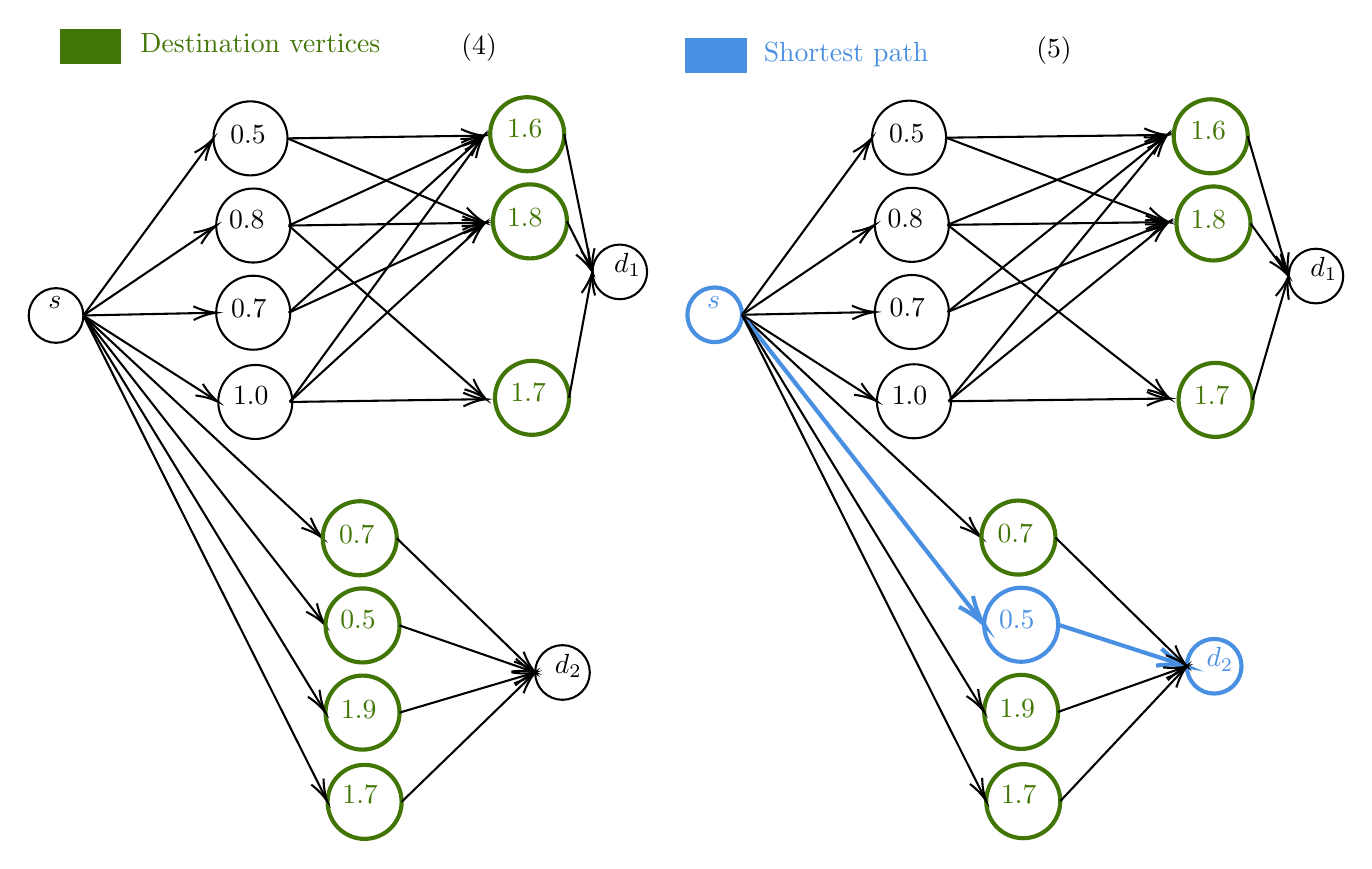
\begin{tikzpicture}[x=0.75pt,y=0.75pt,yscale=-1,xscale=1]
%uncomment if require: \path (0,421); %set diagram left start at 0, and has height of 421

%Shape: Circle [id:dp03935086715862224] 
\draw   (18,151.83) .. controls (18,144.56) and (23.89,138.67) .. (31.17,138.67) .. controls (38.44,138.67) and (44.33,144.56) .. (44.33,151.83) .. controls (44.33,159.11) and (38.44,165) .. (31.17,165) .. controls (23.89,165) and (18,159.11) .. (18,151.83) -- cycle ;
%Shape: Circle [id:dp013741846345812991] 
\draw  [color={rgb, 255:red, 0; green, 0; blue, 0 }  ,draw opacity=1 ] (107,66.5) .. controls (107,56.65) and (114.98,48.67) .. (124.83,48.67) .. controls (134.68,48.67) and (142.67,56.65) .. (142.67,66.5) .. controls (142.67,76.35) and (134.68,84.33) .. (124.83,84.33) .. controls (114.98,84.33) and (107,76.35) .. (107,66.5) -- cycle ;
%Straight Lines [id:da2285961150540936] 
\draw    (44.33,151.83) -- (105.82,68.11) ;
\draw [shift={(107,66.5)}, rotate = 126.29] [color={rgb, 255:red, 0; green, 0; blue, 0 }  ][line width=0.75]    (10.93,-3.29) .. controls (6.95,-1.4) and (3.31,-0.3) .. (0,0) .. controls (3.31,0.3) and (6.95,1.4) .. (10.93,3.29)   ;
%Straight Lines [id:da3172568568087528] 
\draw    (44.33,151.83) -- (106.68,109.62) ;
\draw [shift={(108.33,108.5)}, rotate = 145.9] [color={rgb, 255:red, 0; green, 0; blue, 0 }  ][line width=0.75]    (10.93,-3.29) .. controls (6.95,-1.4) and (3.31,-0.3) .. (0,0) .. controls (3.31,0.3) and (6.95,1.4) .. (10.93,3.29)   ;
%Straight Lines [id:da882921640626438] 
\draw    (142.67,66.5) -- (235.28,65.19) ;
\draw [shift={(237.28,65.17)}, rotate = 179.19] [color={rgb, 255:red, 0; green, 0; blue, 0 }  ][line width=0.75]    (10.93,-3.29) .. controls (6.95,-1.4) and (3.31,-0.3) .. (0,0) .. controls (3.31,0.3) and (6.95,1.4) .. (10.93,3.29)   ;
%Straight Lines [id:da3183274130809055] 
\draw    (143.72,193.5) -- (236.1,66.78) ;
\draw [shift={(237.28,65.17)}, rotate = 126.09] [color={rgb, 255:red, 0; green, 0; blue, 0 }  ][line width=0.75]    (10.93,-3.29) .. controls (6.95,-1.4) and (3.31,-0.3) .. (0,0) .. controls (3.31,0.3) and (6.95,1.4) .. (10.93,3.29)   ;
%Straight Lines [id:da29569959304432225] 
\draw    (44.33,151.83) -- (106.33,150.54) ;
\draw [shift={(108.33,150.5)}, rotate = 178.81] [color={rgb, 255:red, 0; green, 0; blue, 0 }  ][line width=0.75]    (10.93,-3.29) .. controls (6.95,-1.4) and (3.31,-0.3) .. (0,0) .. controls (3.31,0.3) and (6.95,1.4) .. (10.93,3.29)   ;
%Straight Lines [id:da3631073563511207] 
\draw    (44.33,151.83) -- (158.2,257.8) ;
\draw [shift={(159.67,259.17)}, rotate = 222.94] [color={rgb, 255:red, 0; green, 0; blue, 0 }  ][line width=0.75]    (10.93,-3.29) .. controls (6.95,-1.4) and (3.31,-0.3) .. (0,0) .. controls (3.31,0.3) and (6.95,1.4) .. (10.93,3.29)   ;
%Straight Lines [id:da28102771226082557] 
\draw    (44.33,151.83) -- (159.77,299.59) ;
\draw [shift={(161,301.17)}, rotate = 232] [color={rgb, 255:red, 0; green, 0; blue, 0 }  ][line width=0.75]    (10.93,-3.29) .. controls (6.95,-1.4) and (3.31,-0.3) .. (0,0) .. controls (3.31,0.3) and (6.95,1.4) .. (10.93,3.29)   ;
%Shape: Circle [id:dp24756933953413762] 
\draw  [color={rgb, 255:red, 0; green, 0; blue, 0 }  ,draw opacity=1 ] (108.33,108.5) .. controls (108.33,98.65) and (116.32,90.67) .. (126.17,90.67) .. controls (136.02,90.67) and (144,98.65) .. (144,108.5) .. controls (144,118.35) and (136.02,126.33) .. (126.17,126.33) .. controls (116.32,126.33) and (108.33,118.35) .. (108.33,108.5) -- cycle ;
%Shape: Circle [id:dp45921123638840333] 
\draw  [color={rgb, 255:red, 0; green, 0; blue, 0 }  ,draw opacity=1 ] (108.33,150.5) .. controls (108.33,140.65) and (116.32,132.67) .. (126.17,132.67) .. controls (136.02,132.67) and (144,140.65) .. (144,150.5) .. controls (144,160.35) and (136.02,168.33) .. (126.17,168.33) .. controls (116.32,168.33) and (108.33,160.35) .. (108.33,150.5) -- cycle ;
%Shape: Circle [id:dp500925992999105] 
\draw  [color={rgb, 255:red, 0; green, 0; blue, 0 }  ,draw opacity=1 ] (109.33,193.5) .. controls (109.33,183.65) and (117.32,175.67) .. (127.17,175.67) .. controls (137.02,175.67) and (145,183.65) .. (145,193.5) .. controls (145,203.35) and (137.02,211.33) .. (127.17,211.33) .. controls (117.32,211.33) and (109.33,203.35) .. (109.33,193.5) -- cycle ;
%Straight Lines [id:da411477758033586] 
\draw    (44.33,151.83) -- (107.65,192.42) ;
\draw [shift={(109.33,193.5)}, rotate = 212.66] [color={rgb, 255:red, 0; green, 0; blue, 0 }  ][line width=0.75]    (10.93,-3.29) .. controls (6.95,-1.4) and (3.31,-0.3) .. (0,0) .. controls (3.31,0.3) and (6.95,1.4) .. (10.93,3.29)   ;
%Straight Lines [id:da28692837065025323] 
\draw    (143.27,150.5) -- (235.8,66.51) ;
\draw [shift={(237.28,65.17)}, rotate = 137.77] [color={rgb, 255:red, 0; green, 0; blue, 0 }  ][line width=0.75]    (10.93,-3.29) .. controls (6.95,-1.4) and (3.31,-0.3) .. (0,0) .. controls (3.31,0.3) and (6.95,1.4) .. (10.93,3.29)   ;
%Straight Lines [id:da9413376827017845] 
\draw    (143.27,108.5) -- (235.46,66) ;
\draw [shift={(237.28,65.17)}, rotate = 155.25] [color={rgb, 255:red, 0; green, 0; blue, 0 }  ][line width=0.75]    (10.93,-3.29) .. controls (6.95,-1.4) and (3.31,-0.3) .. (0,0) .. controls (3.31,0.3) and (6.95,1.4) .. (10.93,3.29)   ;
%Shape: Circle [id:dp6695824949533475] 
\draw  [color={rgb, 255:red, 65; green, 117; blue, 5 }  ,draw opacity=1 ][line width=1.5]  (240.33,64.5) .. controls (240.33,54.65) and (248.32,46.67) .. (258.17,46.67) .. controls (268.02,46.67) and (276,54.65) .. (276,64.5) .. controls (276,74.35) and (268.02,82.33) .. (258.17,82.33) .. controls (248.32,82.33) and (240.33,74.35) .. (240.33,64.5) -- cycle ;
%Shape: Circle [id:dp289258607486234] 
\draw  [color={rgb, 255:red, 65; green, 117; blue, 5 }  ,draw opacity=1 ][line width=1.5]  (241.67,106.5) .. controls (241.67,96.65) and (249.65,88.67) .. (259.5,88.67) .. controls (269.35,88.67) and (277.33,96.65) .. (277.33,106.5) .. controls (277.33,116.35) and (269.35,124.33) .. (259.5,124.33) .. controls (249.65,124.33) and (241.67,116.35) .. (241.67,106.5) -- cycle ;
%Shape: Circle [id:dp9587031696155075] 
\draw  [color={rgb, 255:red, 65; green, 117; blue, 5 }  ,draw opacity=1 ][line width=1.5]  (242.67,191.5) .. controls (242.67,181.65) and (250.65,173.67) .. (260.5,173.67) .. controls (270.35,173.67) and (278.33,181.65) .. (278.33,191.5) .. controls (278.33,201.35) and (270.35,209.33) .. (260.5,209.33) .. controls (250.65,209.33) and (242.67,201.35) .. (242.67,191.5) -- cycle ;
%Shape: Circle [id:dp8911978431362768] 
\draw  [color={rgb, 255:red, 65; green, 117; blue, 5 }  ,draw opacity=1 ][line width=1.5]  (159.67,259.17) .. controls (159.67,249.32) and (167.65,241.33) .. (177.5,241.33) .. controls (187.35,241.33) and (195.33,249.32) .. (195.33,259.17) .. controls (195.33,269.02) and (187.35,277) .. (177.5,277) .. controls (167.65,277) and (159.67,269.02) .. (159.67,259.17) -- cycle ;
%Shape: Circle [id:dp09192693547917963] 
\draw  [color={rgb, 255:red, 65; green, 117; blue, 5 }  ,draw opacity=1 ][line width=1.5]  (161,301.17) .. controls (161,291.32) and (168.98,283.33) .. (178.83,283.33) .. controls (188.68,283.33) and (196.67,291.32) .. (196.67,301.17) .. controls (196.67,311.02) and (188.68,319) .. (178.83,319) .. controls (168.98,319) and (161,311.02) .. (161,301.17) -- cycle ;
%Shape: Circle [id:dp6972000905493723] 
\draw  [color={rgb, 255:red, 65; green, 117; blue, 5 }  ,draw opacity=1 ][line width=1.5]  (161,343.17) .. controls (161,333.32) and (168.98,325.33) .. (178.83,325.33) .. controls (188.68,325.33) and (196.67,333.32) .. (196.67,343.17) .. controls (196.67,353.02) and (188.68,361) .. (178.83,361) .. controls (168.98,361) and (161,353.02) .. (161,343.17) -- cycle ;
%Shape: Circle [id:dp32409047662252766] 
\draw  [color={rgb, 255:red, 65; green, 117; blue, 5 }  ,draw opacity=1 ][line width=1.5]  (162,386.17) .. controls (162,376.32) and (169.98,368.33) .. (179.83,368.33) .. controls (189.68,368.33) and (197.67,376.32) .. (197.67,386.17) .. controls (197.67,396.02) and (189.68,404) .. (179.83,404) .. controls (169.98,404) and (162,396.02) .. (162,386.17) -- cycle ;
%Straight Lines [id:da7834067530949043] 
\draw    (44.33,151.83) -- (159.96,341.46) ;
\draw [shift={(161,343.17)}, rotate = 238.63] [color={rgb, 255:red, 0; green, 0; blue, 0 }  ][line width=0.75]    (10.93,-3.29) .. controls (6.95,-1.4) and (3.31,-0.3) .. (0,0) .. controls (3.31,0.3) and (6.95,1.4) .. (10.93,3.29)   ;
%Straight Lines [id:da030952050159580802] 
\draw    (44.33,151.83) -- (161.1,384.38) ;
\draw [shift={(162,386.17)}, rotate = 243.34] [color={rgb, 255:red, 0; green, 0; blue, 0 }  ][line width=0.75]    (10.93,-3.29) .. controls (6.95,-1.4) and (3.31,-0.3) .. (0,0) .. controls (3.31,0.3) and (6.95,1.4) .. (10.93,3.29)   ;
%Straight Lines [id:da0532388401921462] 
\draw    (142.67,66.5) -- (236.04,106.38) ;
\draw [shift={(237.88,107.17)}, rotate = 203.13] [color={rgb, 255:red, 0; green, 0; blue, 0 }  ][line width=0.75]    (10.93,-3.29) .. controls (6.95,-1.4) and (3.31,-0.3) .. (0,0) .. controls (3.31,0.3) and (6.95,1.4) .. (10.93,3.29)   ;
%Straight Lines [id:da23022117495331407] 
\draw    (143.27,108.5) -- (235.88,107.19) ;
\draw [shift={(237.88,107.17)}, rotate = 179.19] [color={rgb, 255:red, 0; green, 0; blue, 0 }  ][line width=0.75]    (10.93,-3.29) .. controls (6.95,-1.4) and (3.31,-0.3) .. (0,0) .. controls (3.31,0.3) and (6.95,1.4) .. (10.93,3.29)   ;
%Straight Lines [id:da530571304547885] 
\draw    (143.27,108.5) -- (236.83,190.85) ;
\draw [shift={(238.33,192.17)}, rotate = 221.35] [color={rgb, 255:red, 0; green, 0; blue, 0 }  ][line width=0.75]    (10.93,-3.29) .. controls (6.95,-1.4) and (3.31,-0.3) .. (0,0) .. controls (3.31,0.3) and (6.95,1.4) .. (10.93,3.29)   ;
%Straight Lines [id:da6849384393503726] 
\draw    (143.27,150.5) -- (236.06,108) ;
\draw [shift={(237.88,107.17)}, rotate = 155.39] [color={rgb, 255:red, 0; green, 0; blue, 0 }  ][line width=0.75]    (10.93,-3.29) .. controls (6.95,-1.4) and (3.31,-0.3) .. (0,0) .. controls (3.31,0.3) and (6.95,1.4) .. (10.93,3.29)   ;
%Straight Lines [id:da6054700257002728] 
\draw    (143.72,193.5) -- (236.41,108.52) ;
\draw [shift={(237.88,107.17)}, rotate = 137.48] [color={rgb, 255:red, 0; green, 0; blue, 0 }  ][line width=0.75]    (10.93,-3.29) .. controls (6.95,-1.4) and (3.31,-0.3) .. (0,0) .. controls (3.31,0.3) and (6.95,1.4) .. (10.93,3.29)   ;
%Straight Lines [id:da048525240366936506] 
\draw    (143.72,193.5) -- (236.33,192.19) ;
\draw [shift={(238.33,192.17)}, rotate = 179.19] [color={rgb, 255:red, 0; green, 0; blue, 0 }  ][line width=0.75]    (10.93,-3.29) .. controls (6.95,-1.4) and (3.31,-0.3) .. (0,0) .. controls (3.31,0.3) and (6.95,1.4) .. (10.93,3.29)   ;
%Shape: Rectangle [id:dp3145061470259034] 
\draw  [draw opacity=0][fill={rgb, 255:red, 65; green, 117; blue, 5 }  ,fill opacity=1 ] (33,13.67) -- (62.67,13.67) -- (62.67,30.67) -- (33,30.67) -- cycle ;
%Shape: Circle [id:dp5223227559354211] 
\draw  [color={rgb, 255:red, 74; green, 144; blue, 226 }  ,draw opacity=1 ][line width=1.5]  (335.33,151.5) .. controls (335.33,144.23) and (341.23,138.33) .. (348.5,138.33) .. controls (355.77,138.33) and (361.67,144.23) .. (361.67,151.5) .. controls (361.67,158.77) and (355.77,164.67) .. (348.5,164.67) .. controls (341.23,164.67) and (335.33,158.77) .. (335.33,151.5) -- cycle ;
%Shape: Circle [id:dp8235490358820139] 
\draw  [color={rgb, 255:red, 0; green, 0; blue, 0 }  ,draw opacity=1 ] (424.33,66.17) .. controls (424.33,56.32) and (432.32,48.33) .. (442.17,48.33) .. controls (452.02,48.33) and (460,56.32) .. (460,66.17) .. controls (460,76.02) and (452.02,84) .. (442.17,84) .. controls (432.32,84) and (424.33,76.02) .. (424.33,66.17) -- cycle ;
%Straight Lines [id:da7999108562438766] 
\draw    (361.67,151.5) -- (423.15,67.78) ;
\draw [shift={(424.33,66.17)}, rotate = 126.29] [color={rgb, 255:red, 0; green, 0; blue, 0 }  ][line width=0.75]    (10.93,-3.29) .. controls (6.95,-1.4) and (3.31,-0.3) .. (0,0) .. controls (3.31,0.3) and (6.95,1.4) .. (10.93,3.29)   ;
%Straight Lines [id:da837043140248309] 
\draw    (361.67,151.5) -- (424.01,109.29) ;
\draw [shift={(425.67,108.17)}, rotate = 145.9] [color={rgb, 255:red, 0; green, 0; blue, 0 }  ][line width=0.75]    (10.93,-3.29) .. controls (6.95,-1.4) and (3.31,-0.3) .. (0,0) .. controls (3.31,0.3) and (6.95,1.4) .. (10.93,3.29)   ;
%Straight Lines [id:da2614530736466021] 
\draw    (460,66.17) -- (564.48,64.86) ;
\draw [shift={(566.48,64.83)}, rotate = 179.28] [color={rgb, 255:red, 0; green, 0; blue, 0 }  ][line width=0.75]    (10.93,-3.29) .. controls (6.95,-1.4) and (3.31,-0.3) .. (0,0) .. controls (3.31,0.3) and (6.95,1.4) .. (10.93,3.29)   ;
%Straight Lines [id:da27706787842045877] 
\draw    (461.19,193.17) -- (565.21,66.38) ;
\draw [shift={(566.48,64.83)}, rotate = 129.37] [color={rgb, 255:red, 0; green, 0; blue, 0 }  ][line width=0.75]    (10.93,-3.29) .. controls (6.95,-1.4) and (3.31,-0.3) .. (0,0) .. controls (3.31,0.3) and (6.95,1.4) .. (10.93,3.29)   ;
%Straight Lines [id:da40369956351723424] 
\draw    (361.67,151.5) -- (423.67,150.21) ;
\draw [shift={(425.67,150.17)}, rotate = 178.81] [color={rgb, 255:red, 0; green, 0; blue, 0 }  ][line width=0.75]    (10.93,-3.29) .. controls (6.95,-1.4) and (3.31,-0.3) .. (0,0) .. controls (3.31,0.3) and (6.95,1.4) .. (10.93,3.29)   ;
%Straight Lines [id:da9511140374399076] 
\draw    (361.67,151.5) -- (475.54,257.47) ;
\draw [shift={(477,258.83)}, rotate = 222.94] [color={rgb, 255:red, 0; green, 0; blue, 0 }  ][line width=0.75]    (10.93,-3.29) .. controls (6.95,-1.4) and (3.31,-0.3) .. (0,0) .. controls (3.31,0.3) and (6.95,1.4) .. (10.93,3.29)   ;
%Straight Lines [id:da24500664072618927] 
\draw [color={rgb, 255:red, 74; green, 144; blue, 226 }  ,draw opacity=1 ][line width=1.5]    (361.67,151.5) -- (476.49,298.47) ;
\draw [shift={(478.33,300.83)}, rotate = 232] [color={rgb, 255:red, 74; green, 144; blue, 226 }  ,draw opacity=1 ][line width=1.5]    (14.21,-4.28) .. controls (9.04,-1.82) and (4.3,-0.39) .. (0,0) .. controls (4.3,0.39) and (9.04,1.82) .. (14.21,4.28)   ;
%Shape: Circle [id:dp4442251606309311] 
\draw  [color={rgb, 255:red, 0; green, 0; blue, 0 }  ,draw opacity=1 ] (425.67,108.17) .. controls (425.67,98.32) and (433.65,90.33) .. (443.5,90.33) .. controls (453.35,90.33) and (461.33,98.32) .. (461.33,108.17) .. controls (461.33,118.02) and (453.35,126) .. (443.5,126) .. controls (433.65,126) and (425.67,118.02) .. (425.67,108.17) -- cycle ;
%Shape: Circle [id:dp8073832400567702] 
\draw  [color={rgb, 255:red, 0; green, 0; blue, 0 }  ,draw opacity=1 ] (425.67,150.17) .. controls (425.67,140.32) and (433.65,132.33) .. (443.5,132.33) .. controls (453.35,132.33) and (461.33,140.32) .. (461.33,150.17) .. controls (461.33,160.02) and (453.35,168) .. (443.5,168) .. controls (433.65,168) and (425.67,160.02) .. (425.67,150.17) -- cycle ;
%Shape: Circle [id:dp5027342139428135] 
\draw  [color={rgb, 255:red, 0; green, 0; blue, 0 }  ,draw opacity=1 ] (426.67,193.17) .. controls (426.67,183.32) and (434.65,175.33) .. (444.5,175.33) .. controls (454.35,175.33) and (462.33,183.32) .. (462.33,193.17) .. controls (462.33,203.02) and (454.35,211) .. (444.5,211) .. controls (434.65,211) and (426.67,203.02) .. (426.67,193.17) -- cycle ;
%Straight Lines [id:da3573382000781211] 
\draw    (361.67,151.5) -- (424.98,192.09) ;
\draw [shift={(426.67,193.17)}, rotate = 212.66] [color={rgb, 255:red, 0; green, 0; blue, 0 }  ][line width=0.75]    (10.93,-3.29) .. controls (6.95,-1.4) and (3.31,-0.3) .. (0,0) .. controls (3.31,0.3) and (6.95,1.4) .. (10.93,3.29)   ;
%Straight Lines [id:da36858564874723254] 
\draw    (460.68,150.17) -- (564.92,66.09) ;
\draw [shift={(566.48,64.83)}, rotate = 141.11] [color={rgb, 255:red, 0; green, 0; blue, 0 }  ][line width=0.75]    (10.93,-3.29) .. controls (6.95,-1.4) and (3.31,-0.3) .. (0,0) .. controls (3.31,0.3) and (6.95,1.4) .. (10.93,3.29)   ;
%Straight Lines [id:da4426152056223407] 
\draw    (460.68,108.17) -- (564.63,65.59) ;
\draw [shift={(566.48,64.83)}, rotate = 157.73] [color={rgb, 255:red, 0; green, 0; blue, 0 }  ][line width=0.75]    (10.93,-3.29) .. controls (6.95,-1.4) and (3.31,-0.3) .. (0,0) .. controls (3.31,0.3) and (6.95,1.4) .. (10.93,3.29)   ;
%Shape: Circle [id:dp9669010455588687] 
\draw  [color={rgb, 255:red, 65; green, 117; blue, 5 }  ,draw opacity=1 ][line width=1.5]  (569.67,65.5) .. controls (569.67,55.65) and (577.65,47.67) .. (587.5,47.67) .. controls (597.35,47.67) and (605.33,55.65) .. (605.33,65.5) .. controls (605.33,75.35) and (597.35,83.33) .. (587.5,83.33) .. controls (577.65,83.33) and (569.67,75.35) .. (569.67,65.5) -- cycle ;
%Shape: Circle [id:dp8802634959890325] 
\draw  [color={rgb, 255:red, 65; green, 117; blue, 5 }  ,draw opacity=1 ][line width=1.5]  (571,107.5) .. controls (571,97.65) and (578.98,89.67) .. (588.83,89.67) .. controls (598.68,89.67) and (606.67,97.65) .. (606.67,107.5) .. controls (606.67,117.35) and (598.68,125.33) .. (588.83,125.33) .. controls (578.98,125.33) and (571,117.35) .. (571,107.5) -- cycle ;
%Shape: Circle [id:dp5145564775008538] 
\draw  [color={rgb, 255:red, 65; green, 117; blue, 5 }  ,draw opacity=1 ][line width=1.5]  (572,192.5) .. controls (572,182.65) and (579.98,174.67) .. (589.83,174.67) .. controls (599.68,174.67) and (607.67,182.65) .. (607.67,192.5) .. controls (607.67,202.35) and (599.68,210.33) .. (589.83,210.33) .. controls (579.98,210.33) and (572,202.35) .. (572,192.5) -- cycle ;
%Shape: Circle [id:dp997904016446409] 
\draw  [color={rgb, 255:red, 65; green, 117; blue, 5 }  ,draw opacity=1 ][line width=1.5]  (477,258.83) .. controls (477,248.98) and (484.98,241) .. (494.83,241) .. controls (504.68,241) and (512.67,248.98) .. (512.67,258.83) .. controls (512.67,268.68) and (504.68,276.67) .. (494.83,276.67) .. controls (484.98,276.67) and (477,268.68) .. (477,258.83) -- cycle ;
%Shape: Circle [id:dp11237959565832889] 
\draw  [color={rgb, 255:red, 74; green, 144; blue, 226 }  ,draw opacity=1 ][line width=1.5]  (478.33,300.83) .. controls (478.33,290.98) and (486.32,283) .. (496.17,283) .. controls (506.02,283) and (514,290.98) .. (514,300.83) .. controls (514,310.68) and (506.02,318.67) .. (496.17,318.67) .. controls (486.32,318.67) and (478.33,310.68) .. (478.33,300.83) -- cycle ;
%Shape: Circle [id:dp36007282120318496] 
\draw  [color={rgb, 255:red, 65; green, 117; blue, 5 }  ,draw opacity=1 ][line width=1.5]  (478.33,342.83) .. controls (478.33,332.98) and (486.32,325) .. (496.17,325) .. controls (506.02,325) and (514,332.98) .. (514,342.83) .. controls (514,352.68) and (506.02,360.67) .. (496.17,360.67) .. controls (486.32,360.67) and (478.33,352.68) .. (478.33,342.83) -- cycle ;
%Shape: Circle [id:dp7776148512657146] 
\draw  [color={rgb, 255:red, 65; green, 117; blue, 5 }  ,draw opacity=1 ][line width=1.5]  (479.33,385.83) .. controls (479.33,375.98) and (487.32,368) .. (497.17,368) .. controls (507.02,368) and (515,375.98) .. (515,385.83) .. controls (515,395.68) and (507.02,403.67) .. (497.17,403.67) .. controls (487.32,403.67) and (479.33,395.68) .. (479.33,385.83) -- cycle ;
%Straight Lines [id:da7871296564069374] 
\draw    (361.67,151.5) -- (477.29,341.13) ;
\draw [shift={(478.33,342.83)}, rotate = 238.63] [color={rgb, 255:red, 0; green, 0; blue, 0 }  ][line width=0.75]    (10.93,-3.29) .. controls (6.95,-1.4) and (3.31,-0.3) .. (0,0) .. controls (3.31,0.3) and (6.95,1.4) .. (10.93,3.29)   ;
%Straight Lines [id:da6853254595224183] 
\draw    (361.67,151.5) -- (478.44,384.05) ;
\draw [shift={(479.33,385.83)}, rotate = 243.34] [color={rgb, 255:red, 0; green, 0; blue, 0 }  ][line width=0.75]    (10.93,-3.29) .. controls (6.95,-1.4) and (3.31,-0.3) .. (0,0) .. controls (3.31,0.3) and (6.95,1.4) .. (10.93,3.29)   ;
%Straight Lines [id:da670866704222034] 
\draw    (460,66.17) -- (565.29,106.12) ;
\draw [shift={(567.16,106.83)}, rotate = 200.78] [color={rgb, 255:red, 0; green, 0; blue, 0 }  ][line width=0.75]    (10.93,-3.29) .. controls (6.95,-1.4) and (3.31,-0.3) .. (0,0) .. controls (3.31,0.3) and (6.95,1.4) .. (10.93,3.29)   ;
%Straight Lines [id:da7187971755911626] 
\draw    (460.68,108.17) -- (565.16,106.86) ;
\draw [shift={(567.16,106.83)}, rotate = 179.28] [color={rgb, 255:red, 0; green, 0; blue, 0 }  ][line width=0.75]    (10.93,-3.29) .. controls (6.95,-1.4) and (3.31,-0.3) .. (0,0) .. controls (3.31,0.3) and (6.95,1.4) .. (10.93,3.29)   ;
%Straight Lines [id:da6885624695484318] 
\draw    (460.68,108.17) -- (566.09,190.6) ;
\draw [shift={(567.67,191.83)}, rotate = 218.03] [color={rgb, 255:red, 0; green, 0; blue, 0 }  ][line width=0.75]    (10.93,-3.29) .. controls (6.95,-1.4) and (3.31,-0.3) .. (0,0) .. controls (3.31,0.3) and (6.95,1.4) .. (10.93,3.29)   ;
%Straight Lines [id:da9859598819774635] 
\draw    (460.68,150.17) -- (565.3,107.59) ;
\draw [shift={(567.16,106.83)}, rotate = 157.86] [color={rgb, 255:red, 0; green, 0; blue, 0 }  ][line width=0.75]    (10.93,-3.29) .. controls (6.95,-1.4) and (3.31,-0.3) .. (0,0) .. controls (3.31,0.3) and (6.95,1.4) .. (10.93,3.29)   ;
%Straight Lines [id:da140803981648562] 
\draw    (461.19,193.17) -- (565.61,108.1) ;
\draw [shift={(567.16,106.83)}, rotate = 140.83] [color={rgb, 255:red, 0; green, 0; blue, 0 }  ][line width=0.75]    (10.93,-3.29) .. controls (6.95,-1.4) and (3.31,-0.3) .. (0,0) .. controls (3.31,0.3) and (6.95,1.4) .. (10.93,3.29)   ;
%Straight Lines [id:da8142768182305606] 
\draw    (461.19,193.17) -- (565.67,191.86) ;
\draw [shift={(567.67,191.83)}, rotate = 179.28] [color={rgb, 255:red, 0; green, 0; blue, 0 }  ][line width=0.75]    (10.93,-3.29) .. controls (6.95,-1.4) and (3.31,-0.3) .. (0,0) .. controls (3.31,0.3) and (6.95,1.4) .. (10.93,3.29)   ;
%Shape: Rectangle [id:dp4032682866148172] 
\draw  [draw opacity=0][fill={rgb, 255:red, 74; green, 144; blue, 226 }  ,fill opacity=1 ] (334.33,18) -- (364,18) -- (364,35) -- (334.33,35) -- cycle ;
%Shape: Circle [id:dp18401472911101835] 
\draw  [color={rgb, 255:red, 74; green, 144; blue, 226 }  ,draw opacity=1 ][line width=1.5]  (576,320.83) .. controls (576,313.56) and (581.89,307.67) .. (589.17,307.67) .. controls (596.44,307.67) and (602.33,313.56) .. (602.33,320.83) .. controls (602.33,328.11) and (596.44,334) .. (589.17,334) .. controls (581.89,334) and (576,328.11) .. (576,320.83) -- cycle ;
%Straight Lines [id:da4476244061779746] 
\draw [color={rgb, 255:red, 74; green, 144; blue, 226 }  ,draw opacity=1 ][line width=1.5]    (514,300.83) -- (573.14,319.91) ;
\draw [shift={(576,320.83)}, rotate = 197.88] [color={rgb, 255:red, 74; green, 144; blue, 226 }  ,draw opacity=1 ][line width=1.5]    (14.21,-4.28) .. controls (9.04,-1.82) and (4.3,-0.39) .. (0,0) .. controls (4.3,0.39) and (9.04,1.82) .. (14.21,4.28)   ;
%Straight Lines [id:da5557730566162855] 
\draw    (512.67,258.83) -- (574.57,319.43) ;
\draw [shift={(576,320.83)}, rotate = 224.39] [color={rgb, 255:red, 0; green, 0; blue, 0 }  ][line width=0.75]    (10.93,-3.29) .. controls (6.95,-1.4) and (3.31,-0.3) .. (0,0) .. controls (3.31,0.3) and (6.95,1.4) .. (10.93,3.29)   ;
%Straight Lines [id:da3360188569236937] 
\draw    (514,342.83) -- (574.12,321.5) ;
\draw [shift={(576,320.83)}, rotate = 160.46] [color={rgb, 255:red, 0; green, 0; blue, 0 }  ][line width=0.75]    (10.93,-3.29) .. controls (6.95,-1.4) and (3.31,-0.3) .. (0,0) .. controls (3.31,0.3) and (6.95,1.4) .. (10.93,3.29)   ;
%Straight Lines [id:da5974529976062386] 
\draw    (515,385.83) -- (574.63,322.29) ;
\draw [shift={(576,320.83)}, rotate = 133.18] [color={rgb, 255:red, 0; green, 0; blue, 0 }  ][line width=0.75]    (10.93,-3.29) .. controls (6.95,-1.4) and (3.31,-0.3) .. (0,0) .. controls (3.31,0.3) and (6.95,1.4) .. (10.93,3.29)   ;
%Shape: Circle [id:dp5339734373389766] 
\draw   (625,132.83) .. controls (625,125.56) and (630.89,119.67) .. (638.17,119.67) .. controls (645.44,119.67) and (651.33,125.56) .. (651.33,132.83) .. controls (651.33,140.11) and (645.44,146) .. (638.17,146) .. controls (630.89,146) and (625,140.11) .. (625,132.83) -- cycle ;
%Straight Lines [id:da2484267262945794] 
\draw    (605.33,65.5) -- (624.44,130.91) ;
\draw [shift={(625,132.83)}, rotate = 253.72] [color={rgb, 255:red, 0; green, 0; blue, 0 }  ][line width=0.75]    (10.93,-3.29) .. controls (6.95,-1.4) and (3.31,-0.3) .. (0,0) .. controls (3.31,0.3) and (6.95,1.4) .. (10.93,3.29)   ;
%Straight Lines [id:da15923057569426224] 
\draw    (606.67,107.5) -- (623.83,131.21) ;
\draw [shift={(625,132.83)}, rotate = 234.11] [color={rgb, 255:red, 0; green, 0; blue, 0 }  ][line width=0.75]    (10.93,-3.29) .. controls (6.95,-1.4) and (3.31,-0.3) .. (0,0) .. controls (3.31,0.3) and (6.95,1.4) .. (10.93,3.29)   ;
%Straight Lines [id:da06869854729567448] 
\draw    (607.67,192.5) -- (624.44,134.75) ;
\draw [shift={(625,132.83)}, rotate = 106.2] [color={rgb, 255:red, 0; green, 0; blue, 0 }  ][line width=0.75]    (10.93,-3.29) .. controls (6.95,-1.4) and (3.31,-0.3) .. (0,0) .. controls (3.31,0.3) and (6.95,1.4) .. (10.93,3.29)   ;
%Shape: Circle [id:dp05217765289720355] 
\draw   (262,323.83) .. controls (262,316.56) and (267.89,310.67) .. (275.17,310.67) .. controls (282.44,310.67) and (288.33,316.56) .. (288.33,323.83) .. controls (288.33,331.11) and (282.44,337) .. (275.17,337) .. controls (267.89,337) and (262,331.11) .. (262,323.83) -- cycle ;
%Straight Lines [id:da5780668053991489] 
\draw    (195.33,259.17) -- (260.56,322.44) ;
\draw [shift={(262,323.83)}, rotate = 224.13] [color={rgb, 255:red, 0; green, 0; blue, 0 }  ][line width=0.75]    (10.93,-3.29) .. controls (6.95,-1.4) and (3.31,-0.3) .. (0,0) .. controls (3.31,0.3) and (6.95,1.4) .. (10.93,3.29)   ;
%Straight Lines [id:da3295236619125801] 
\draw    (196.67,301.17) -- (260.11,323.18) ;
\draw [shift={(262,323.83)}, rotate = 199.13] [color={rgb, 255:red, 0; green, 0; blue, 0 }  ][line width=0.75]    (10.93,-3.29) .. controls (6.95,-1.4) and (3.31,-0.3) .. (0,0) .. controls (3.31,0.3) and (6.95,1.4) .. (10.93,3.29)   ;
%Straight Lines [id:da4600994870971551] 
\draw    (196.67,343.17) -- (260.08,324.4) ;
\draw [shift={(262,323.83)}, rotate = 163.52] [color={rgb, 255:red, 0; green, 0; blue, 0 }  ][line width=0.75]    (10.93,-3.29) .. controls (6.95,-1.4) and (3.31,-0.3) .. (0,0) .. controls (3.31,0.3) and (6.95,1.4) .. (10.93,3.29)   ;
%Straight Lines [id:da6183291898243775] 
\draw    (197.67,386.17) -- (260.56,325.23) ;
\draw [shift={(262,323.83)}, rotate = 135.9] [color={rgb, 255:red, 0; green, 0; blue, 0 }  ][line width=0.75]    (10.93,-3.29) .. controls (6.95,-1.4) and (3.31,-0.3) .. (0,0) .. controls (3.31,0.3) and (6.95,1.4) .. (10.93,3.29)   ;
%Shape: Circle [id:dp7050921731028599] 
\draw   (289.6,130.83) .. controls (289.6,123.56) and (295.49,117.67) .. (302.77,117.67) .. controls (310.04,117.67) and (315.93,123.56) .. (315.93,130.83) .. controls (315.93,138.11) and (310.04,144) .. (302.77,144) .. controls (295.49,144) and (289.6,138.11) .. (289.6,130.83) -- cycle ;
%Straight Lines [id:da528718432407641] 
\draw    (276,64.5) -- (289.2,128.87) ;
\draw [shift={(289.6,130.83)}, rotate = 258.41] [color={rgb, 255:red, 0; green, 0; blue, 0 }  ][line width=0.75]    (10.93,-3.29) .. controls (6.95,-1.4) and (3.31,-0.3) .. (0,0) .. controls (3.31,0.3) and (6.95,1.4) .. (10.93,3.29)   ;
%Straight Lines [id:da363537493706525] 
\draw    (277.33,106.5) -- (288.7,129.05) ;
\draw [shift={(289.6,130.83)}, rotate = 243.25] [color={rgb, 255:red, 0; green, 0; blue, 0 }  ][line width=0.75]    (10.93,-3.29) .. controls (6.95,-1.4) and (3.31,-0.3) .. (0,0) .. controls (3.31,0.3) and (6.95,1.4) .. (10.93,3.29)   ;
%Straight Lines [id:da8788904508041877] 
\draw    (278.33,191.5) -- (289.23,132.8) ;
\draw [shift={(289.6,130.83)}, rotate = 100.52] [color={rgb, 255:red, 0; green, 0; blue, 0 }  ][line width=0.75]    (10.93,-3.29) .. controls (6.95,-1.4) and (3.31,-0.3) .. (0,0) .. controls (3.31,0.3) and (6.95,1.4) .. (10.93,3.29)   ;

% Text Node
\draw (113.67,58.73) node [anchor=north west][inner sep=0.75pt]  [color={rgb, 255:red, 0; green, 0; blue, 0 }  ,opacity=1 ]  {$0.5$};
% Text Node
\draw (113,99.73) node [anchor=north west][inner sep=0.75pt]  [color={rgb, 255:red, 0; green, 0; blue, 0 }  ,opacity=1 ]  {$0.8$};
% Text Node
\draw (114,142.73) node [anchor=north west][inner sep=0.75pt]  [color={rgb, 255:red, 0; green, 0; blue, 0 }  ,opacity=1 ]  {$0.7$};
% Text Node
\draw (115,184.73) node [anchor=north west][inner sep=0.75pt]  [color={rgb, 255:red, 0; green, 0; blue, 0 }  ,opacity=1 ]  {$1.0$};
% Text Node
\draw (26,141.4) node [anchor=north west][inner sep=0.75pt]    {$s$};
% Text Node
\draw (70.33,14.33) node [anchor=north west][inner sep=0.75pt]  [color={rgb, 255:red, 65; green, 117; blue, 5 }  ,opacity=1 ] [align=left] {Destination vertices};
% Text Node
\draw (247,56.07) node [anchor=north west][inner sep=0.75pt]  [color={rgb, 255:red, 65; green, 117; blue, 5 }  ,opacity=1 ]  {$1.6$};
% Text Node
\draw (247,98.73) node [anchor=north west][inner sep=0.75pt]  [color={rgb, 255:red, 65; green, 117; blue, 5 }  ,opacity=1 ]  {$1.8$};
% Text Node
\draw (248.67,183.4) node [anchor=north west][inner sep=0.75pt]  [color={rgb, 255:red, 65; green, 117; blue, 5 }  ,opacity=1 ]  {$1.7$};
% Text Node
\draw (166,251.4) node [anchor=north west][inner sep=0.75pt]  [color={rgb, 255:red, 65; green, 117; blue, 5 }  ,opacity=1 ]  {$0.7$};
% Text Node
\draw (166.67,292.73) node [anchor=north west][inner sep=0.75pt]  [color={rgb, 255:red, 65; green, 117; blue, 5 }  ,opacity=1 ]  {$0.5$};
% Text Node
\draw (167,335.73) node [anchor=north west][inner sep=0.75pt]  [color={rgb, 255:red, 65; green, 117; blue, 5 }  ,opacity=1 ]  {$1.9$};
% Text Node
\draw (167.67,377.07) node [anchor=north west][inner sep=0.75pt]  [color={rgb, 255:red, 65; green, 117; blue, 5 }  ,opacity=1 ]  {$1.7$};
% Text Node
\draw (431,58.4) node [anchor=north west][inner sep=0.75pt]  [color={rgb, 255:red, 0; green, 0; blue, 0 }  ,opacity=1 ]  {$0.5$};
% Text Node
\draw (430.33,99.4) node [anchor=north west][inner sep=0.75pt]  [color={rgb, 255:red, 0; green, 0; blue, 0 }  ,opacity=1 ]  {$0.8$};
% Text Node
\draw (431.33,142.4) node [anchor=north west][inner sep=0.75pt]  [color={rgb, 255:red, 0; green, 0; blue, 0 }  ,opacity=1 ]  {$0.7$};
% Text Node
\draw (432.33,184.4) node [anchor=north west][inner sep=0.75pt]  [color={rgb, 255:red, 0; green, 0; blue, 0 }  ,opacity=1 ]  {$1.0$};
% Text Node
\draw (343.33,141.07) node [anchor=north west][inner sep=0.75pt]  [color={rgb, 255:red, 74; green, 144; blue, 226 }  ,opacity=1 ]  {$s$};
% Text Node
\draw (576.33,57.07) node [anchor=north west][inner sep=0.75pt]  [color={rgb, 255:red, 65; green, 117; blue, 5 }  ,opacity=1 ]  {$1.6$};
% Text Node
\draw (576.33,99.73) node [anchor=north west][inner sep=0.75pt]  [color={rgb, 255:red, 65; green, 117; blue, 5 }  ,opacity=1 ]  {$1.8$};
% Text Node
\draw (578,184.4) node [anchor=north west][inner sep=0.75pt]  [color={rgb, 255:red, 65; green, 117; blue, 5 }  ,opacity=1 ]  {$1.7$};
% Text Node
\draw (483.33,251.07) node [anchor=north west][inner sep=0.75pt]  [color={rgb, 255:red, 65; green, 117; blue, 5 }  ,opacity=1 ]  {$0.7$};
% Text Node
\draw (484,292.4) node [anchor=north west][inner sep=0.75pt]  [color={rgb, 255:red, 74; green, 144; blue, 226 }  ,opacity=1 ]  {$0.5$};
% Text Node
\draw (484.33,335.4) node [anchor=north west][inner sep=0.75pt]  [color={rgb, 255:red, 65; green, 117; blue, 5 }  ,opacity=1 ]  {$1.9$};
% Text Node
\draw (485,376.73) node [anchor=north west][inner sep=0.75pt]  [color={rgb, 255:red, 65; green, 117; blue, 5 }  ,opacity=1 ]  {$1.7$};
% Text Node
\draw (370.67,18.67) node [anchor=north west][inner sep=0.75pt]  [color={rgb, 255:red, 74; green, 144; blue, 226 }  ,opacity=1 ] [align=left] {Shortest path};
% Text Node
\draw (584,310.4) node [anchor=north west][inner sep=0.75pt]  [color={rgb, 255:red, 74; green, 144; blue, 226 }  ,opacity=1 ]  {$d_{2}$};
% Text Node
\draw (634,122.4) node [anchor=north west][inner sep=0.75pt]    {$d_{1}$};
% Text Node
\draw (270,313.4) node [anchor=north west][inner sep=0.75pt]    {$d_{2}$};
% Text Node
\draw (298.6,120.4) node [anchor=north west][inner sep=0.75pt]    {$d_{1}$};
% Text Node
\draw (225,14.71) node [anchor=north west][inner sep=0.75pt]   [align=left] {(4)};
% Text Node
\draw (502,16) node [anchor=north west][inner sep=0.75pt]   [align=left] {(5)};


\end{tikzpicture}




\tikzset{every picture/.style={line width=0.75pt}} %set default line width to 0.75pt        

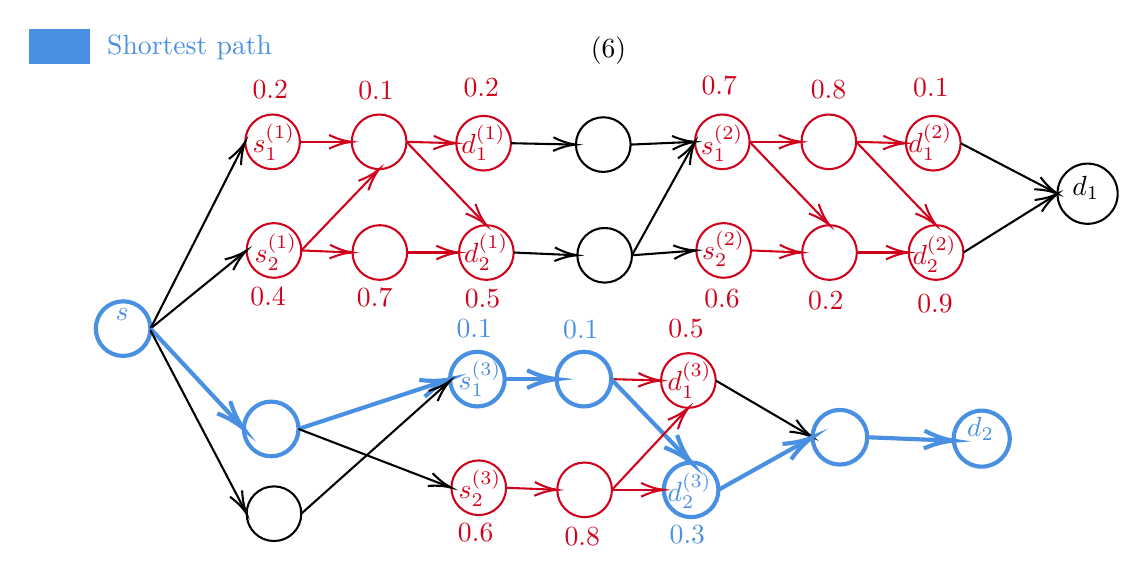
\begin{tikzpicture}[x=0.75pt,y=0.75pt,yscale=-1,xscale=1]
%uncomment if require: \path (0,278); %set diagram left start at 0, and has height of 278

%Shape: Circle [id:dp4186788365931191] 
\draw  [color={rgb, 255:red, 74; green, 144; blue, 226 }  ,draw opacity=1 ][line width=1.5]  (97,152.17) .. controls (97,144.89) and (102.89,139) .. (110.17,139) .. controls (117.44,139) and (123.33,144.89) .. (123.33,152.17) .. controls (123.33,159.44) and (117.44,165.33) .. (110.17,165.33) .. controls (102.89,165.33) and (97,159.44) .. (97,152.17) -- cycle ;
%Shape: Circle [id:dp7763921207597995] 
\draw   (560.33,87.17) .. controls (560.33,79.16) and (566.83,72.67) .. (574.83,72.67) .. controls (582.84,72.67) and (589.33,79.16) .. (589.33,87.17) .. controls (589.33,95.17) and (582.84,101.67) .. (574.83,101.67) .. controls (566.83,101.67) and (560.33,95.17) .. (560.33,87.17) -- cycle ;
%Shape: Circle [id:dp8835122956709349] 
\draw  [color={rgb, 255:red, 74; green, 144; blue, 226 }  ,draw opacity=1 ][line width=1.5]  (510.33,205.17) .. controls (510.33,197.71) and (516.38,191.67) .. (523.83,191.67) .. controls (531.29,191.67) and (537.33,197.71) .. (537.33,205.17) .. controls (537.33,212.62) and (531.29,218.67) .. (523.83,218.67) .. controls (516.38,218.67) and (510.33,212.62) .. (510.33,205.17) -- cycle ;
%Shape: Circle [id:dp5299468800784968] 
\draw  [color={rgb, 255:red, 208; green, 2; blue, 27 }  ,draw opacity=1 ] (169,62.17) .. controls (169,54.89) and (174.89,49) .. (182.17,49) .. controls (189.44,49) and (195.33,54.89) .. (195.33,62.17) .. controls (195.33,69.44) and (189.44,75.33) .. (182.17,75.33) .. controls (174.89,75.33) and (169,69.44) .. (169,62.17) -- cycle ;
%Shape: Circle [id:dp26255788220721454] 
\draw  [color={rgb, 255:red, 208; green, 2; blue, 27 }  ,draw opacity=1 ] (220.33,62.17) .. controls (220.33,54.89) and (226.23,49) .. (233.5,49) .. controls (240.77,49) and (246.67,54.89) .. (246.67,62.17) .. controls (246.67,69.44) and (240.77,75.33) .. (233.5,75.33) .. controls (226.23,75.33) and (220.33,69.44) .. (220.33,62.17) -- cycle ;
%Shape: Circle [id:dp476142137064856] 
\draw  [color={rgb, 255:red, 208; green, 2; blue, 27 }  ,draw opacity=1 ] (270.67,62.83) .. controls (270.67,55.56) and (276.56,49.67) .. (283.83,49.67) .. controls (291.11,49.67) and (297,55.56) .. (297,62.83) .. controls (297,70.11) and (291.11,76) .. (283.83,76) .. controls (276.56,76) and (270.67,70.11) .. (270.67,62.83) -- cycle ;
%Shape: Circle [id:dp5840063911525781] 
\draw  [color={rgb, 255:red, 208; green, 2; blue, 27 }  ,draw opacity=1 ] (169.67,114.5) .. controls (169.67,107.23) and (175.56,101.33) .. (182.83,101.33) .. controls (190.11,101.33) and (196,107.23) .. (196,114.5) .. controls (196,121.77) and (190.11,127.67) .. (182.83,127.67) .. controls (175.56,127.67) and (169.67,121.77) .. (169.67,114.5) -- cycle ;
%Shape: Circle [id:dp0353814239710315] 
\draw  [color={rgb, 255:red, 208; green, 2; blue, 27 }  ,draw opacity=1 ] (220.67,115.5) .. controls (220.67,108.23) and (226.56,102.33) .. (233.83,102.33) .. controls (241.11,102.33) and (247,108.23) .. (247,115.5) .. controls (247,122.77) and (241.11,128.67) .. (233.83,128.67) .. controls (226.56,128.67) and (220.67,122.77) .. (220.67,115.5) -- cycle ;
%Shape: Circle [id:dp6363071493887607] 
\draw  [color={rgb, 255:red, 208; green, 2; blue, 27 }  ,draw opacity=1 ] (272,115.5) .. controls (272,108.23) and (277.89,102.33) .. (285.17,102.33) .. controls (292.44,102.33) and (298.33,108.23) .. (298.33,115.5) .. controls (298.33,122.77) and (292.44,128.67) .. (285.17,128.67) .. controls (277.89,128.67) and (272,122.77) .. (272,115.5) -- cycle ;
%Straight Lines [id:da24175484014306825] 
\draw [color={rgb, 255:red, 208; green, 2; blue, 27 }  ,draw opacity=1 ]   (195.33,62.17) -- (218.33,62.17) ;
\draw [shift={(220.33,62.17)}, rotate = 180] [color={rgb, 255:red, 208; green, 2; blue, 27 }  ,draw opacity=1 ][line width=0.75]    (10.93,-3.29) .. controls (6.95,-1.4) and (3.31,-0.3) .. (0,0) .. controls (3.31,0.3) and (6.95,1.4) .. (10.93,3.29)   ;
%Straight Lines [id:da8124523539919186] 
\draw [color={rgb, 255:red, 208; green, 2; blue, 27 }  ,draw opacity=1 ]   (246.67,62.17) -- (268.67,62.78) ;
\draw [shift={(270.67,62.83)}, rotate = 181.59] [color={rgb, 255:red, 208; green, 2; blue, 27 }  ,draw opacity=1 ][line width=0.75]    (10.93,-3.29) .. controls (6.95,-1.4) and (3.31,-0.3) .. (0,0) .. controls (3.31,0.3) and (6.95,1.4) .. (10.93,3.29)   ;
%Straight Lines [id:da05198621718190055] 
\draw [color={rgb, 255:red, 208; green, 2; blue, 27 }  ,draw opacity=1 ]   (196,114.5) -- (218.67,115.42) ;
\draw [shift={(220.67,115.5)}, rotate = 182.32] [color={rgb, 255:red, 208; green, 2; blue, 27 }  ,draw opacity=1 ][line width=0.75]    (10.93,-3.29) .. controls (6.95,-1.4) and (3.31,-0.3) .. (0,0) .. controls (3.31,0.3) and (6.95,1.4) .. (10.93,3.29)   ;
%Straight Lines [id:da5045956688106266] 
\draw [color={rgb, 255:red, 208; green, 2; blue, 27 }  ,draw opacity=1 ]   (247,115.5) -- (270,115.5) ;
\draw [shift={(272,115.5)}, rotate = 180] [color={rgb, 255:red, 208; green, 2; blue, 27 }  ,draw opacity=1 ][line width=0.75]    (10.93,-3.29) .. controls (6.95,-1.4) and (3.31,-0.3) .. (0,0) .. controls (3.31,0.3) and (6.95,1.4) .. (10.93,3.29)   ;
%Straight Lines [id:da20978089880313244] 
\draw [color={rgb, 255:red, 208; green, 2; blue, 27 }  ,draw opacity=1 ]   (246.67,62.17) -- (283.78,100.89) ;
\draw [shift={(285.17,102.33)}, rotate = 226.21] [color={rgb, 255:red, 208; green, 2; blue, 27 }  ,draw opacity=1 ][line width=0.75]    (10.93,-3.29) .. controls (6.95,-1.4) and (3.31,-0.3) .. (0,0) .. controls (3.31,0.3) and (6.95,1.4) .. (10.93,3.29)   ;
%Straight Lines [id:da742925172047987] 
\draw [color={rgb, 255:red, 208; green, 2; blue, 27 }  ,draw opacity=1 ]   (196,114.5) -- (232.12,76.78) ;
\draw [shift={(233.5,75.33)}, rotate = 133.75] [color={rgb, 255:red, 208; green, 2; blue, 27 }  ,draw opacity=1 ][line width=0.75]    (10.93,-3.29) .. controls (6.95,-1.4) and (3.31,-0.3) .. (0,0) .. controls (3.31,0.3) and (6.95,1.4) .. (10.93,3.29)   ;
%Shape: Circle [id:dp9940407825585735] 
\draw  [color={rgb, 255:red, 208; green, 2; blue, 27 }  ,draw opacity=1 ] (385.67,62.17) .. controls (385.67,54.89) and (391.56,49) .. (398.83,49) .. controls (406.11,49) and (412,54.89) .. (412,62.17) .. controls (412,69.44) and (406.11,75.33) .. (398.83,75.33) .. controls (391.56,75.33) and (385.67,69.44) .. (385.67,62.17) -- cycle ;
%Shape: Circle [id:dp16581146895545507] 
\draw  [color={rgb, 255:red, 208; green, 2; blue, 27 }  ,draw opacity=1 ] (437,62.17) .. controls (437,54.89) and (442.89,49) .. (450.17,49) .. controls (457.44,49) and (463.33,54.89) .. (463.33,62.17) .. controls (463.33,69.44) and (457.44,75.33) .. (450.17,75.33) .. controls (442.89,75.33) and (437,69.44) .. (437,62.17) -- cycle ;
%Shape: Circle [id:dp07684466599238049] 
\draw  [color={rgb, 255:red, 208; green, 2; blue, 27 }  ,draw opacity=1 ] (487.33,62.83) .. controls (487.33,55.56) and (493.23,49.67) .. (500.5,49.67) .. controls (507.77,49.67) and (513.67,55.56) .. (513.67,62.83) .. controls (513.67,70.11) and (507.77,76) .. (500.5,76) .. controls (493.23,76) and (487.33,70.11) .. (487.33,62.83) -- cycle ;
%Shape: Circle [id:dp3025016135910288] 
\draw  [color={rgb, 255:red, 208; green, 2; blue, 27 }  ,draw opacity=1 ] (386.33,114.5) .. controls (386.33,107.23) and (392.23,101.33) .. (399.5,101.33) .. controls (406.77,101.33) and (412.67,107.23) .. (412.67,114.5) .. controls (412.67,121.77) and (406.77,127.67) .. (399.5,127.67) .. controls (392.23,127.67) and (386.33,121.77) .. (386.33,114.5) -- cycle ;
%Shape: Circle [id:dp6852099828928286] 
\draw  [color={rgb, 255:red, 208; green, 2; blue, 27 }  ,draw opacity=1 ] (437.33,115.5) .. controls (437.33,108.23) and (443.23,102.33) .. (450.5,102.33) .. controls (457.77,102.33) and (463.67,108.23) .. (463.67,115.5) .. controls (463.67,122.77) and (457.77,128.67) .. (450.5,128.67) .. controls (443.23,128.67) and (437.33,122.77) .. (437.33,115.5) -- cycle ;
%Shape: Circle [id:dp7094319274264116] 
\draw  [color={rgb, 255:red, 208; green, 2; blue, 27 }  ,draw opacity=1 ] (488.67,115.5) .. controls (488.67,108.23) and (494.56,102.33) .. (501.83,102.33) .. controls (509.11,102.33) and (515,108.23) .. (515,115.5) .. controls (515,122.77) and (509.11,128.67) .. (501.83,128.67) .. controls (494.56,128.67) and (488.67,122.77) .. (488.67,115.5) -- cycle ;
%Straight Lines [id:da5436708414248501] 
\draw [color={rgb, 255:red, 208; green, 2; blue, 27 }  ,draw opacity=1 ]   (412,62.17) -- (435,62.17) ;
\draw [shift={(437,62.17)}, rotate = 180] [color={rgb, 255:red, 208; green, 2; blue, 27 }  ,draw opacity=1 ][line width=0.75]    (10.93,-3.29) .. controls (6.95,-1.4) and (3.31,-0.3) .. (0,0) .. controls (3.31,0.3) and (6.95,1.4) .. (10.93,3.29)   ;
%Straight Lines [id:da3139908829816431] 
\draw [color={rgb, 255:red, 208; green, 2; blue, 27 }  ,draw opacity=1 ]   (463.33,62.17) -- (485.33,62.78) ;
\draw [shift={(487.33,62.83)}, rotate = 181.59] [color={rgb, 255:red, 208; green, 2; blue, 27 }  ,draw opacity=1 ][line width=0.75]    (10.93,-3.29) .. controls (6.95,-1.4) and (3.31,-0.3) .. (0,0) .. controls (3.31,0.3) and (6.95,1.4) .. (10.93,3.29)   ;
%Straight Lines [id:da5217620576111766] 
\draw [color={rgb, 255:red, 208; green, 2; blue, 27 }  ,draw opacity=1 ]   (412.67,114.5) -- (435.33,115.42) ;
\draw [shift={(437.33,115.5)}, rotate = 182.32] [color={rgb, 255:red, 208; green, 2; blue, 27 }  ,draw opacity=1 ][line width=0.75]    (10.93,-3.29) .. controls (6.95,-1.4) and (3.31,-0.3) .. (0,0) .. controls (3.31,0.3) and (6.95,1.4) .. (10.93,3.29)   ;
%Straight Lines [id:da8706941656241487] 
\draw [color={rgb, 255:red, 208; green, 2; blue, 27 }  ,draw opacity=1 ]   (463.67,115.5) -- (486.67,115.5) ;
\draw [shift={(488.67,115.5)}, rotate = 180] [color={rgb, 255:red, 208; green, 2; blue, 27 }  ,draw opacity=1 ][line width=0.75]    (10.93,-3.29) .. controls (6.95,-1.4) and (3.31,-0.3) .. (0,0) .. controls (3.31,0.3) and (6.95,1.4) .. (10.93,3.29)   ;
%Straight Lines [id:da12364438400419187] 
\draw [color={rgb, 255:red, 208; green, 2; blue, 27 }  ,draw opacity=1 ]   (412,62.17) -- (449.12,100.89) ;
\draw [shift={(450.5,102.33)}, rotate = 226.21] [color={rgb, 255:red, 208; green, 2; blue, 27 }  ,draw opacity=1 ][line width=0.75]    (10.93,-3.29) .. controls (6.95,-1.4) and (3.31,-0.3) .. (0,0) .. controls (3.31,0.3) and (6.95,1.4) .. (10.93,3.29)   ;
%Straight Lines [id:da9380593529898558] 
\draw [color={rgb, 255:red, 208; green, 2; blue, 27 }  ,draw opacity=1 ]   (463.33,62.17) -- (500.45,100.89) ;
\draw [shift={(501.83,102.33)}, rotate = 226.21] [color={rgb, 255:red, 208; green, 2; blue, 27 }  ,draw opacity=1 ][line width=0.75]    (10.93,-3.29) .. controls (6.95,-1.4) and (3.31,-0.3) .. (0,0) .. controls (3.31,0.3) and (6.95,1.4) .. (10.93,3.29)   ;
%Shape: Circle [id:dp7960081269353008] 
\draw  [color={rgb, 255:red, 74; green, 144; blue, 226 }  ,draw opacity=1 ][line width=1.5]  (267.67,176.5) .. controls (267.67,169.23) and (273.56,163.33) .. (280.83,163.33) .. controls (288.11,163.33) and (294,169.23) .. (294,176.5) .. controls (294,183.77) and (288.11,189.67) .. (280.83,189.67) .. controls (273.56,189.67) and (267.67,183.77) .. (267.67,176.5) -- cycle ;
%Shape: Circle [id:dp4060658645183488] 
\draw  [color={rgb, 255:red, 74; green, 144; blue, 226 }  ,draw opacity=1 ][line width=1.5]  (319,176.5) .. controls (319,169.23) and (324.89,163.33) .. (332.17,163.33) .. controls (339.44,163.33) and (345.33,169.23) .. (345.33,176.5) .. controls (345.33,183.77) and (339.44,189.67) .. (332.17,189.67) .. controls (324.89,189.67) and (319,183.77) .. (319,176.5) -- cycle ;
%Shape: Circle [id:dp3579925259435661] 
\draw  [color={rgb, 255:red, 208; green, 2; blue, 27 }  ,draw opacity=1 ] (369.33,177.17) .. controls (369.33,169.89) and (375.23,164) .. (382.5,164) .. controls (389.77,164) and (395.67,169.89) .. (395.67,177.17) .. controls (395.67,184.44) and (389.77,190.33) .. (382.5,190.33) .. controls (375.23,190.33) and (369.33,184.44) .. (369.33,177.17) -- cycle ;
%Shape: Circle [id:dp6459182021434369] 
\draw  [color={rgb, 255:red, 208; green, 2; blue, 27 }  ,draw opacity=1 ] (268.33,228.83) .. controls (268.33,221.56) and (274.23,215.67) .. (281.5,215.67) .. controls (288.77,215.67) and (294.67,221.56) .. (294.67,228.83) .. controls (294.67,236.11) and (288.77,242) .. (281.5,242) .. controls (274.23,242) and (268.33,236.11) .. (268.33,228.83) -- cycle ;
%Shape: Circle [id:dp7191560598537521] 
\draw  [color={rgb, 255:red, 208; green, 2; blue, 27 }  ,draw opacity=1 ] (319.33,229.83) .. controls (319.33,222.56) and (325.23,216.67) .. (332.5,216.67) .. controls (339.77,216.67) and (345.67,222.56) .. (345.67,229.83) .. controls (345.67,237.11) and (339.77,243) .. (332.5,243) .. controls (325.23,243) and (319.33,237.11) .. (319.33,229.83) -- cycle ;
%Shape: Circle [id:dp8748814774304257] 
\draw  [color={rgb, 255:red, 74; green, 144; blue, 226 }  ,draw opacity=1 ][line width=1.5]  (370.67,229.83) .. controls (370.67,222.56) and (376.56,216.67) .. (383.83,216.67) .. controls (391.11,216.67) and (397,222.56) .. (397,229.83) .. controls (397,237.11) and (391.11,243) .. (383.83,243) .. controls (376.56,243) and (370.67,237.11) .. (370.67,229.83) -- cycle ;
%Straight Lines [id:da6253633238181582] 
\draw [color={rgb, 255:red, 74; green, 144; blue, 226 }  ,draw opacity=1 ][line width=1.5]    (294,176.5) -- (316,176.5) ;
\draw [shift={(319,176.5)}, rotate = 180] [color={rgb, 255:red, 74; green, 144; blue, 226 }  ,draw opacity=1 ][line width=1.5]    (14.21,-4.28) .. controls (9.04,-1.82) and (4.3,-0.39) .. (0,0) .. controls (4.3,0.39) and (9.04,1.82) .. (14.21,4.28)   ;
%Straight Lines [id:da2200785017209579] 
\draw [color={rgb, 255:red, 208; green, 2; blue, 27 }  ,draw opacity=1 ]   (345.33,176.5) -- (367.33,177.11) ;
\draw [shift={(369.33,177.17)}, rotate = 181.59] [color={rgb, 255:red, 208; green, 2; blue, 27 }  ,draw opacity=1 ][line width=0.75]    (10.93,-3.29) .. controls (6.95,-1.4) and (3.31,-0.3) .. (0,0) .. controls (3.31,0.3) and (6.95,1.4) .. (10.93,3.29)   ;
%Straight Lines [id:da8233944524716443] 
\draw [color={rgb, 255:red, 208; green, 2; blue, 27 }  ,draw opacity=1 ]   (294.67,228.83) -- (317.33,229.75) ;
\draw [shift={(319.33,229.83)}, rotate = 182.32] [color={rgb, 255:red, 208; green, 2; blue, 27 }  ,draw opacity=1 ][line width=0.75]    (10.93,-3.29) .. controls (6.95,-1.4) and (3.31,-0.3) .. (0,0) .. controls (3.31,0.3) and (6.95,1.4) .. (10.93,3.29)   ;
%Straight Lines [id:da6883932774145891] 
\draw [color={rgb, 255:red, 208; green, 2; blue, 27 }  ,draw opacity=1 ]   (345.67,229.83) -- (368.67,229.83) ;
\draw [shift={(370.67,229.83)}, rotate = 180] [color={rgb, 255:red, 208; green, 2; blue, 27 }  ,draw opacity=1 ][line width=0.75]    (10.93,-3.29) .. controls (6.95,-1.4) and (3.31,-0.3) .. (0,0) .. controls (3.31,0.3) and (6.95,1.4) .. (10.93,3.29)   ;
%Straight Lines [id:da9775419946298616] 
\draw [color={rgb, 255:red, 74; green, 144; blue, 226 }  ,draw opacity=1 ][line width=1.5]    (345.33,176.5) -- (381.76,214.5) ;
\draw [shift={(383.83,216.67)}, rotate = 226.21] [color={rgb, 255:red, 74; green, 144; blue, 226 }  ,draw opacity=1 ][line width=1.5]    (14.21,-4.28) .. controls (9.04,-1.82) and (4.3,-0.39) .. (0,0) .. controls (4.3,0.39) and (9.04,1.82) .. (14.21,4.28)   ;
%Straight Lines [id:da17393283871253318] 
\draw [color={rgb, 255:red, 208; green, 2; blue, 27 }  ,draw opacity=1 ]   (345.67,229.83) -- (381.14,191.8) ;
\draw [shift={(382.5,190.33)}, rotate = 133] [color={rgb, 255:red, 208; green, 2; blue, 27 }  ,draw opacity=1 ][line width=0.75]    (10.93,-3.29) .. controls (6.95,-1.4) and (3.31,-0.3) .. (0,0) .. controls (3.31,0.3) and (6.95,1.4) .. (10.93,3.29)   ;
%Shape: Circle [id:dp7840849303162021] 
\draw  [color={rgb, 255:red, 74; green, 144; blue, 226 }  ,draw opacity=1 ][line width=1.5]  (168.33,200.5) .. controls (168.33,193.23) and (174.23,187.33) .. (181.5,187.33) .. controls (188.77,187.33) and (194.67,193.23) .. (194.67,200.5) .. controls (194.67,207.77) and (188.77,213.67) .. (181.5,213.67) .. controls (174.23,213.67) and (168.33,207.77) .. (168.33,200.5) -- cycle ;
%Shape: Circle [id:dp7967550977032296] 
\draw   (329,116.83) .. controls (329,109.56) and (334.89,103.67) .. (342.17,103.67) .. controls (349.44,103.67) and (355.33,109.56) .. (355.33,116.83) .. controls (355.33,124.11) and (349.44,130) .. (342.17,130) .. controls (334.89,130) and (329,124.11) .. (329,116.83) -- cycle ;
%Shape: Circle [id:dp5183655656627832] 
\draw   (328.33,63.5) .. controls (328.33,56.23) and (334.23,50.33) .. (341.5,50.33) .. controls (348.77,50.33) and (354.67,56.23) .. (354.67,63.5) .. controls (354.67,70.77) and (348.77,76.67) .. (341.5,76.67) .. controls (334.23,76.67) and (328.33,70.77) .. (328.33,63.5) -- cycle ;
%Shape: Circle [id:dp22816341609622426] 
\draw  [color={rgb, 255:red, 74; green, 144; blue, 226 }  ,draw opacity=1 ][line width=1.5]  (442.33,204.5) .. controls (442.33,197.23) and (448.23,191.33) .. (455.5,191.33) .. controls (462.77,191.33) and (468.67,197.23) .. (468.67,204.5) .. controls (468.67,211.77) and (462.77,217.67) .. (455.5,217.67) .. controls (448.23,217.67) and (442.33,211.77) .. (442.33,204.5) -- cycle ;
%Straight Lines [id:da9020817690579448] 
\draw    (123.33,152.17) -- (168.1,63.95) ;
\draw [shift={(169,62.17)}, rotate = 116.9] [color={rgb, 255:red, 0; green, 0; blue, 0 }  ][line width=0.75]    (10.93,-3.29) .. controls (6.95,-1.4) and (3.31,-0.3) .. (0,0) .. controls (3.31,0.3) and (6.95,1.4) .. (10.93,3.29)   ;
%Straight Lines [id:da5783278087821677] 
\draw    (123.33,152.17) -- (168.11,115.76) ;
\draw [shift={(169.67,114.5)}, rotate = 140.89] [color={rgb, 255:red, 0; green, 0; blue, 0 }  ][line width=0.75]    (10.93,-3.29) .. controls (6.95,-1.4) and (3.31,-0.3) .. (0,0) .. controls (3.31,0.3) and (6.95,1.4) .. (10.93,3.29)   ;
%Straight Lines [id:da5906898853515139] 
\draw    (297,62.83) -- (326.33,63.46) ;
\draw [shift={(328.33,63.5)}, rotate = 181.22] [color={rgb, 255:red, 0; green, 0; blue, 0 }  ][line width=0.75]    (10.93,-3.29) .. controls (6.95,-1.4) and (3.31,-0.3) .. (0,0) .. controls (3.31,0.3) and (6.95,1.4) .. (10.93,3.29)   ;
%Straight Lines [id:da018182758062898374] 
\draw    (354.67,63.5) -- (383.67,62.25) ;
\draw [shift={(385.67,62.17)}, rotate = 177.54] [color={rgb, 255:red, 0; green, 0; blue, 0 }  ][line width=0.75]    (10.93,-3.29) .. controls (6.95,-1.4) and (3.31,-0.3) .. (0,0) .. controls (3.31,0.3) and (6.95,1.4) .. (10.93,3.29)   ;
%Straight Lines [id:da011690207492813132] 
\draw    (355.33,116.83) -- (384.34,114.65) ;
\draw [shift={(386.33,114.5)}, rotate = 175.7] [color={rgb, 255:red, 0; green, 0; blue, 0 }  ][line width=0.75]    (10.93,-3.29) .. controls (6.95,-1.4) and (3.31,-0.3) .. (0,0) .. controls (3.31,0.3) and (6.95,1.4) .. (10.93,3.29)   ;
%Straight Lines [id:da7758620683005653] 
\draw    (298.33,115.5) -- (327,116.75) ;
\draw [shift={(329,116.83)}, rotate = 182.49] [color={rgb, 255:red, 0; green, 0; blue, 0 }  ][line width=0.75]    (10.93,-3.29) .. controls (6.95,-1.4) and (3.31,-0.3) .. (0,0) .. controls (3.31,0.3) and (6.95,1.4) .. (10.93,3.29)   ;
%Straight Lines [id:da8061417388960925] 
\draw    (355.33,116.83) -- (384.7,63.92) ;
\draw [shift={(385.67,62.17)}, rotate = 119.02] [color={rgb, 255:red, 0; green, 0; blue, 0 }  ][line width=0.75]    (10.93,-3.29) .. controls (6.95,-1.4) and (3.31,-0.3) .. (0,0) .. controls (3.31,0.3) and (6.95,1.4) .. (10.93,3.29)   ;
%Straight Lines [id:da27973131060906087] 
\draw [color={rgb, 255:red, 74; green, 144; blue, 226 }  ,draw opacity=1 ][line width=1.5]    (123.33,152.17) -- (166.29,198.3) ;
\draw [shift={(168.33,200.5)}, rotate = 227.05] [color={rgb, 255:red, 74; green, 144; blue, 226 }  ,draw opacity=1 ][line width=1.5]    (14.21,-4.28) .. controls (9.04,-1.82) and (4.3,-0.39) .. (0,0) .. controls (4.3,0.39) and (9.04,1.82) .. (14.21,4.28)   ;
%Straight Lines [id:da5987451153417733] 
\draw [color={rgb, 255:red, 74; green, 144; blue, 226 }  ,draw opacity=1 ][line width=1.5]    (194.67,200.5) -- (264.82,177.44) ;
\draw [shift={(267.67,176.5)}, rotate = 161.8] [color={rgb, 255:red, 74; green, 144; blue, 226 }  ,draw opacity=1 ][line width=1.5]    (14.21,-4.28) .. controls (9.04,-1.82) and (4.3,-0.39) .. (0,0) .. controls (4.3,0.39) and (9.04,1.82) .. (14.21,4.28)   ;
%Straight Lines [id:da9370062579490619] 
\draw    (194.67,200.5) -- (266.47,228.12) ;
\draw [shift={(268.33,228.83)}, rotate = 201.04] [color={rgb, 255:red, 0; green, 0; blue, 0 }  ][line width=0.75]    (10.93,-3.29) .. controls (6.95,-1.4) and (3.31,-0.3) .. (0,0) .. controls (3.31,0.3) and (6.95,1.4) .. (10.93,3.29)   ;
%Straight Lines [id:da870662410036803] 
\draw    (395.67,177.17) -- (440.61,203.49) ;
\draw [shift={(442.33,204.5)}, rotate = 210.36] [color={rgb, 255:red, 0; green, 0; blue, 0 }  ][line width=0.75]    (10.93,-3.29) .. controls (6.95,-1.4) and (3.31,-0.3) .. (0,0) .. controls (3.31,0.3) and (6.95,1.4) .. (10.93,3.29)   ;
%Straight Lines [id:da8438607348276028] 
\draw    (513.67,62.83) -- (558.56,86.24) ;
\draw [shift={(560.33,87.17)}, rotate = 207.54] [color={rgb, 255:red, 0; green, 0; blue, 0 }  ][line width=0.75]    (10.93,-3.29) .. controls (6.95,-1.4) and (3.31,-0.3) .. (0,0) .. controls (3.31,0.3) and (6.95,1.4) .. (10.93,3.29)   ;
%Straight Lines [id:da19429197504706264] 
\draw    (515,115.5) -- (558.64,88.23) ;
\draw [shift={(560.33,87.17)}, rotate = 147.99] [color={rgb, 255:red, 0; green, 0; blue, 0 }  ][line width=0.75]    (10.93,-3.29) .. controls (6.95,-1.4) and (3.31,-0.3) .. (0,0) .. controls (3.31,0.3) and (6.95,1.4) .. (10.93,3.29)   ;
%Straight Lines [id:da9952193607979982] 
\draw [color={rgb, 255:red, 74; green, 144; blue, 226 }  ,draw opacity=1 ][line width=1.5]    (397,229.83) -- (439.71,205.96) ;
\draw [shift={(442.33,204.5)}, rotate = 150.8] [color={rgb, 255:red, 74; green, 144; blue, 226 }  ,draw opacity=1 ][line width=1.5]    (14.21,-4.28) .. controls (9.04,-1.82) and (4.3,-0.39) .. (0,0) .. controls (4.3,0.39) and (9.04,1.82) .. (14.21,4.28)   ;
%Straight Lines [id:da22963070389749984] 
\draw [color={rgb, 255:red, 74; green, 144; blue, 226 }  ,draw opacity=1 ][line width=1.5]    (468.67,204.5) -- (507.34,206.05) ;
\draw [shift={(510.33,206.17)}, rotate = 182.29] [color={rgb, 255:red, 74; green, 144; blue, 226 }  ,draw opacity=1 ][line width=1.5]    (14.21,-4.28) .. controls (9.04,-1.82) and (4.3,-0.39) .. (0,0) .. controls (4.3,0.39) and (9.04,1.82) .. (14.21,4.28)   ;
%Shape: Rectangle [id:dp18806194708133805] 
\draw  [draw opacity=0][fill={rgb, 255:red, 74; green, 144; blue, 226 }  ,fill opacity=1 ] (64.67,7.67) -- (94.33,7.67) -- (94.33,24.67) -- (64.67,24.67) -- cycle ;
%Shape: Circle [id:dp7088399825648537] 
\draw   (169.67,241.33) .. controls (169.67,234.06) and (175.56,228.17) .. (182.83,228.17) .. controls (190.11,228.17) and (196,234.06) .. (196,241.33) .. controls (196,248.61) and (190.11,254.5) .. (182.83,254.5) .. controls (175.56,254.5) and (169.67,248.61) .. (169.67,241.33) -- cycle ;
%Straight Lines [id:da4223681583285508] 
\draw    (123.33,153) -- (168.74,239.56) ;
\draw [shift={(169.67,241.33)}, rotate = 242.32] [color={rgb, 255:red, 0; green, 0; blue, 0 }  ][line width=0.75]    (10.93,-3.29) .. controls (6.95,-1.4) and (3.31,-0.3) .. (0,0) .. controls (3.31,0.3) and (6.95,1.4) .. (10.93,3.29)   ;
%Straight Lines [id:da5982587637586831] 
\draw    (196,241.33) -- (266.17,178.67) ;
\draw [shift={(267.67,177.33)}, rotate = 138.23] [color={rgb, 255:red, 0; green, 0; blue, 0 }  ][line width=0.75]    (10.93,-3.29) .. controls (6.95,-1.4) and (3.31,-0.3) .. (0,0) .. controls (3.31,0.3) and (6.95,1.4) .. (10.93,3.29)   ;

% Text Node
\draw (171,52.07) node [anchor=north west][inner sep=0.75pt]  [color={rgb, 255:red, 208; green, 2; blue, 27 }  ,opacity=1 ]  {$s_{1}^{( 1)}$};
% Text Node
\draw (172,105.07) node [anchor=north west][inner sep=0.75pt]  [color={rgb, 255:red, 208; green, 2; blue, 27 }  ,opacity=1 ]  {$s_{2}^{( 1)}$};
% Text Node
\draw (273,105.07) node [anchor=north west][inner sep=0.75pt]  [color={rgb, 255:red, 208; green, 2; blue, 27 }  ,opacity=1 ]  {$d_{2}^{( 1)}$};
% Text Node
\draw (271.67,52.4) node [anchor=north west][inner sep=0.75pt]  [color={rgb, 255:red, 208; green, 2; blue, 27 }  ,opacity=1 ]  {$d_{1}^{( 1)}$};
% Text Node
\draw (270.33,166.07) node [anchor=north west][inner sep=0.75pt]  [color={rgb, 255:red, 74; green, 144; blue, 226 }  ,opacity=1 ]  {$s_{1}^{( 3)}$};
% Text Node
\draw (270.33,218.73) node [anchor=north west][inner sep=0.75pt]  [color={rgb, 255:red, 208; green, 2; blue, 27 }  ,opacity=1 ]  {$s_{2}^{( 3)}$};
% Text Node
\draw (371,166.73) node [anchor=north west][inner sep=0.75pt]  [color={rgb, 255:red, 208; green, 2; blue, 27 }  ,opacity=1 ]  {$d_{1}^{( 3)}$};
% Text Node
\draw (371,220.07) node [anchor=north west][inner sep=0.75pt]  [color={rgb, 255:red, 74; green, 144; blue, 226 }  ,opacity=1 ]  {$d_{2}^{( 3)}$};
% Text Node
\draw (487,52.07) node [anchor=north west][inner sep=0.75pt]  [color={rgb, 255:red, 208; green, 2; blue, 27 }  ,opacity=1 ]  {$d_{1}^{( 2)}$};
% Text Node
\draw (489,106.07) node [anchor=north west][inner sep=0.75pt]  [color={rgb, 255:red, 208; green, 2; blue, 27 }  ,opacity=1 ]  {$d_{2}^{( 2)}$};
% Text Node
\draw (387,52.73) node [anchor=north west][inner sep=0.75pt]  [color={rgb, 255:red, 208; green, 2; blue, 27 }  ,opacity=1 ]  {$s_{1}^{( 2)}$};
% Text Node
\draw (387.67,103.4) node [anchor=north west][inner sep=0.75pt]  [color={rgb, 255:red, 208; green, 2; blue, 27 }  ,opacity=1 ]  {$s_{2}^{( 2)}$};
% Text Node
\draw (105,141.07) node [anchor=north west][inner sep=0.75pt]  [color={rgb, 255:red, 74; green, 144; blue, 226 }  ,opacity=1 ]  {$s$};
% Text Node
\draw (566,77.4) node [anchor=north west][inner sep=0.75pt]    {$d_{1}$};
% Text Node
\draw (515.33,193.4) node [anchor=north west][inner sep=0.75pt]  [color={rgb, 255:red, 74; green, 144; blue, 226 }  ,opacity=1 ]  {$d_{2}$};
% Text Node
\draw (171,31.07) node [anchor=north west][inner sep=0.75pt]  [color={rgb, 255:red, 208; green, 2; blue, 27 }  ,opacity=1 ]  {$0.2$};
% Text Node
\draw (170,130.73) node [anchor=north west][inner sep=0.75pt]  [color={rgb, 255:red, 208; green, 2; blue, 27 }  ,opacity=1 ]  {$0.4$};
% Text Node
\draw (221.33,131.4) node [anchor=north west][inner sep=0.75pt]  [color={rgb, 255:red, 208; green, 2; blue, 27 }  ,opacity=1 ]  {$0.7$};
% Text Node
\draw (222,31.73) node [anchor=north west][inner sep=0.75pt]  [color={rgb, 255:red, 208; green, 2; blue, 27 }  ,opacity=1 ]  {$0.1$};
% Text Node
\draw (272.67,30.4) node [anchor=north west][inner sep=0.75pt]  [color={rgb, 255:red, 208; green, 2; blue, 27 }  ,opacity=1 ]  {$0.2$};
% Text Node
\draw (273.33,131.73) node [anchor=north west][inner sep=0.75pt]  [color={rgb, 255:red, 208; green, 2; blue, 27 }  ,opacity=1 ]  {$0.5$};
% Text Node
\draw (489.33,30.4) node [anchor=north west][inner sep=0.75pt]  [color={rgb, 255:red, 208; green, 2; blue, 27 }  ,opacity=1 ]  {$0.1$};
% Text Node
\draw (440,31.07) node [anchor=north west][inner sep=0.75pt]  [color={rgb, 255:red, 208; green, 2; blue, 27 }  ,opacity=1 ]  {$0.8$};
% Text Node
\draw (387.33,29.07) node [anchor=north west][inner sep=0.75pt]  [color={rgb, 255:red, 208; green, 2; blue, 27 }  ,opacity=1 ]  {$0.7$};
% Text Node
\draw (388.67,131.73) node [anchor=north west][inner sep=0.75pt]  [color={rgb, 255:red, 208; green, 2; blue, 27 }  ,opacity=1 ]  {$0.6$};
% Text Node
\draw (438.67,133.07) node [anchor=north west][inner sep=0.75pt]  [color={rgb, 255:red, 208; green, 2; blue, 27 }  ,opacity=1 ]  {$0.2$};
% Text Node
\draw (491.33,134.4) node [anchor=north west][inner sep=0.75pt]  [color={rgb, 255:red, 208; green, 2; blue, 27 }  ,opacity=1 ]  {$0.9$};
% Text Node
\draw (270,244.4) node [anchor=north west][inner sep=0.75pt]  [color={rgb, 255:red, 208; green, 2; blue, 27 }  ,opacity=1 ]  {$0.6$};
% Text Node
\draw (321.33,246.4) node [anchor=north west][inner sep=0.75pt]  [color={rgb, 255:red, 208; green, 2; blue, 27 }  ,opacity=1 ]  {$0.8$};
% Text Node
\draw (372,245.73) node [anchor=north west][inner sep=0.75pt]  [color={rgb, 255:red, 74; green, 144; blue, 226 }  ,opacity=1 ]  {$0.3$};
% Text Node
\draw (320.67,146.73) node [anchor=north west][inner sep=0.75pt]  [color={rgb, 255:red, 74; green, 144; blue, 226 }  ,opacity=1 ]  {$0.1$};
% Text Node
\draw (269.33,146.4) node [anchor=north west][inner sep=0.75pt]  [color={rgb, 255:red, 74; green, 144; blue, 226 }  ,opacity=1 ]  {$0.1$};
% Text Node
\draw (371.33,146.4) node [anchor=north west][inner sep=0.75pt]  [color={rgb, 255:red, 208; green, 2; blue, 27 }  ,opacity=1 ]  {$0.5$};
% Text Node
\draw (101,9.33) node [anchor=north west][inner sep=0.75pt]  [color={rgb, 255:red, 74; green, 144; blue, 226 }  ,opacity=1 ] [align=left] {Shortest path};
% Text Node
\draw (334,10) node [anchor=north west][inner sep=0.75pt]   [align=left] {(6)};

\end{tikzpicture}
\begin{center}
    Figure 3: High-level Architecture
\end{center}

\textcolor{teal}{\textbf{solution within math notation.}} The input is a graph containing uncertain subgraphs $\{G^{(z)}\}_z$, each represents object uncertainty in the environment. For each subgraph $G^{(z)}$ the shortest-path distance of all pairs $(s_i^{(z)}, d_j^{(z)})$ of local starting and destination vertices gets computed. Those pairs get converted to weighted edges with weights $w_{ij}^{(z)}$ corresponding to shortest-path weights. Each such pair $(s_i^{(z)}, d_j^{(z)})$ gets transformed to a vertex $v_{ij}^{(z)}$ weighted by $w_{ij}^{(z)}$, whereby it has inner edges $(v, v_{ij}^{(z)})$ if there were $(v, s_i^{(z)})$ for all $v$, and has outer edges $(v_{ij}^{(z)}, v)$ if there were $(d_j^{(z)}, v)$. For every pair of vertices $v_{ij}^{(z)}$ and $v_{qp}^{(z')}$, a random path is sampled, and a corresponding edge $(v_{ij}^{(z)}, v_{qp}^{(z')})$ is added. Now we can compute the shortest path to any destination. Through our transformations and computations, a computed path could be reduced back to the original read graph to have a shortest-path.

\textbf{Procedure.}
\begin{itemize}
    \item (1) Read a graph with uncertain subgraphs $\{G^{(z)} \}_z$.
    \item (2) Reduce every uncertain subgraph $G^{(z)}$ to edges $(s_i^{(z)}, d_j^{(z)})$ weighted with the shortest distance $w_{ij}^{(z)}$ between $s_i^{(z)}$ and $d_j^{(z)}$.
    \item (3) For every $z$, reduce every pair $(s_i^{(z)}, d_j^{(z)})$ to vertex $v_{ij}^{(z)}$ weighted by $w_{ij}^{(z)}$. Set inner edges $(v,v_{ij}^{(z)}) \longleftrightarrow (v, s_i) \; \forall v$ and set outer edge $(v_{ij}^{(z)}, v) \longleftrightarrow (d_j, v) \; \forall v$.
    \item (4) For every $v_{ij}^{(z)}$ and $v_{qp}^{(z')}$, find a neutral path from $v_{ij}^{(z)}$ to $v_{qp}^{(z')}$, then set edge $(v_{ij}^{(z)}, v_{qp}^{(z')})$.
    \item (5) Compute a shortest path to any destination.
    \item (6) Output the path but on the original graph, which shows the neutral paths and shortest paths of the uncertain subgraphs altogether.
\end{itemize}

In our implementation, we construct graph (4) immediately from graph (1). Detailed steps are given for a clearer illustration.


\subsection{Vertex-weighted Shortest Path}

\begin{center}
    \begin{tikzpicture}[
    node distance={18mm},
    thick,
    main/.style = {draw, circle, minimum size=7mm}
]
\node[main] (1) {};
\node[main, fill=darkred, fill opacity=0.5] (2) [below left of = 1] {};
\node[main] (3) [below right of = 1] {};
\node[main] (4) [below left of = 2] {};
\node[main] (5) [below right of = 2] {};
\draw[->] (1) -- (2); 
\draw[->] (1) -- (3);
\draw[->] (2) -- (4);
\draw[->] (2) -- (5);
\draw[->] (3) -- (2);
\node[above=0.5mm of 2] {$Ex[X_i]$};
\end{tikzpicture}
\hspace{3mm}
\begin{tikzpicture}[
    node distance={18mm},
    thick,
    main/.style = {draw, circle, minimum size=7mm}
] 
\node[main] (1) {};
\node[main] (2) [below left of = 1] {};
\node[main] (3) [below right of = 1] {};
\node[main] (4) [below left of = 2] {};
\node[main] (5) [below right of = 2] {};
\draw[->, color=darkred] (1) -- node[midway, above left] {$Ex[X_i]$} (2); 
\draw[->] (1) -- (3);
\draw[->] (2) -- (4);
\draw[->] (2) -- (5);
\draw[->, color=darkred] (3) -- node[midway, below] {$Ex[X_i]$} (2);
\node[above=0.5mm of 2] {};
\end{tikzpicture} \\
    Figure 4: Vertex uncertainty to edge weight
\end{center}


\textbf{Definition.} \textit{weight-backward} transformation. Suppose we are given a graph $G$ where the ith vertex is labeled with expectation $Ex[X_i]$. Construct a digraph $G'$ by labeling the edges of $G$ as follows: for every $v_i \in V(G)$, we label an edge $(v_k, v_i)$ by $Ex[v_i]$.

\textbf{Theorem.} If $G$ is transformed to $G'$ by \textit{weight-backward}, then a path $p$ is of expectation $w$ in $G$ iff it is of expectation $w$ in $G'$.

\textit{Proof.} Recall by definition $Ex[X_{root}] = 0$. For the base case where $|p| = 1$, total expectation $Ex[X] = 0$ in $G$. In $G'$, $p$ won't have any edges, so $Ex[X] = 0$ in $G'$ as well.

Assume the statement holds for $k \geq 1$, and consider an arbitrary path $p$ where $|p| = k+1$. Call $p = (v_1, \dots, v_{k+1})$. By hypothesis $\sum_{i=1}^k Ex[X_i] = \sum_{i=2}^k Ex[X_{(v_{i-1}, v_{i})}]$. By definition we have $Ex[X_{k+1}] = Ex[X_{(v_k, v_{k+1})}]$. Hence the inductive step follows as
\begin{align*}
\left ( \sum_{i=1}^k Ex[X_i] \right ) + Ex[X_{k+1}] &= \left ( \sum_{i=2}^k Ex[X_{(v_{i-1}, v_{i})}] \right ) + Ex[X_{(v_k, v_{k+1})}] \\
\sum_{i=1}^{k+1} Ex[X_i] &= \sum_{i=2}^{k+1} Ex[X_{(v_{i-1}, v_{i})}]
\end{align*}

\textbf{Corollary.} For a \textit{directed graph} $G$ and a path $p$, $p$ is minimal or maximal in $G$ if and only if $p$ is minimal or maximal in transformed $G'$.

Follows immediately since ordering is preserved by the previous theorem.

\subsection{Neutral Path} \label{Neutral Path}

The matrix $A$ here is the adjacency matrix of a given digraph $G$ whereby $A[i,j] = 1$ if and only if $(v_i, v_j) \in E(G)$. A useful property of adjacency matrices is that $A^k[i,j]$ is exactly the number of distinct walks of length $k$ from vertex $v_i$ to vertex $v_j$. 

Consider a relation composition $G^k$ where $a G^k b$ iff there is a length-k walk in $G$ from $a$ to $b$. Observe $G^0 \cup G^1 \cup \dots \cup G^{|V(G)|-1} = (G \cup G^0)^{|V(G)|-1}$. Accordingly, if we consider the graph $G \cup G^0$ in place of $G$, with matrix $A + I_n$ in place of $A$, then $A^k[i,j]$ is the number of walks of length at most $k$ from $v_i$ to $v_j$. See \cite{discreteHandbook} for a background.

\textbf{Definition.} boolean dot product, in place dot product

\textbf{Definition.} matrix boolean product $A^{[r]}$, in place matrix multiplication

\textbf{Proposition.} Consider a Matrix multiplication by the dot-product: $v_i \cdot v_j = \bigvee_k \big ( (v_i, v_k) \wedge (v_k, v_j) \big )$. It follows $A^k[a,b] = 1$ iff $a G^k b$, so it decides whether a walk exists instead of counting walks.

\textbf{Proposition.} For $k < n-1$, if $A^k[i,j] = 1$ then there is a path, but if $A^k[i,j] = 0$ then the existence of a path from $i$ to $j$ is undecided.

\textbf{Problem.} Intermediary matrix $M$ on $A^1, A^2, A^4, \dots, A^{2^m}$.

$A^1 = G \cup G^0 = W \vee I$ and $A^{2k} = A^k \cdot A^k$.
\begin{align*}
M^1[i,j] &= \begin{cases} 
      \phi & A^1[i,j]=1, \; i \neq j \\
      Nil & \text{otherwise}
    \end{cases} \\
M^{2k}[i,j] &= \begin{cases} 
      q & A^k[i,q] = 1 = A^k[q,j], \; i,j,q \text{ distinct} \\
      Nil & \text{otherwise}
    \end{cases}
\end{align*}

\textbf{Algorithm}
\begin{verbatim}
# input:  k, power of 2; i & j, M^k[i,j] != Nil
# output: intermediary path between i and j
intermediaryPath(i, j, k)

    # base case. directly connected, then no intermediary path
    if G[i,j] = phi return ()
    
    # not directly connected, then we pick an intermediary vertex
    q = M^k[i,j]
    
    # recursively construct intermediary paths from i to q, and from q to j.
    return pathConstruction(i, q, k/2) + (q) + pathConstruction(q, j, k/2)

# input: k, power of 2; i & j
# output: path from i to j
main(i, j, k)

    # trivial path
    if i == j return (i)

    # directly connected
    if G[i,j] == 1:
        return (i, j)

    # if not directly connected, and no intermediary vertex exists,
    # then no path exists
    if M^k[i,j] == Nil return Nil

    # if an intermediary vertex exists,
    # then so does some intermediate path
    return (i) + intermediaryPath(i, j, k) + (j)
\end{verbatim}

\textit{Correctness Proof.} By strong induction on the length of paths.

For the base case where $|p| = 1$, clearly $i = j$ and we get the right answer.

For the base case where $|p| = 2$, clearly $p = (i,j)$ and $i$ is directly connected to $j$.

Consider a path $p$ such that $|p| = m > 2$ and denote $p = (v_1, v_2, \dots, v_m)$. Assume the algorithm is correct for any path $p$ where $|p| < m$.

For the case of $v_1 \neq v_m$ and $M^k[i,j] \neq Nil$, we know there is an intermediary vertex $q$, with a path $p_0$ from $v_1$ to $q$, and a path $p_1$ from $q$ to $v_m$. Clearly $|p_0| < k$ and $|p_1| < k$, and by induction hypothesis, paths $p_0$ and $p_1$ produced are correct. It follows the path $(v_1) + p_0 + (q) + p_1 + (v_m)$ is correct from $i$ to $j$ as intended.


\subsection{Dynamic Update}

\textbf{Weights}

\begin{center}
    \tikzset{every picture/.style={line width=0.75pt}} %set default line width to 0.75pt        

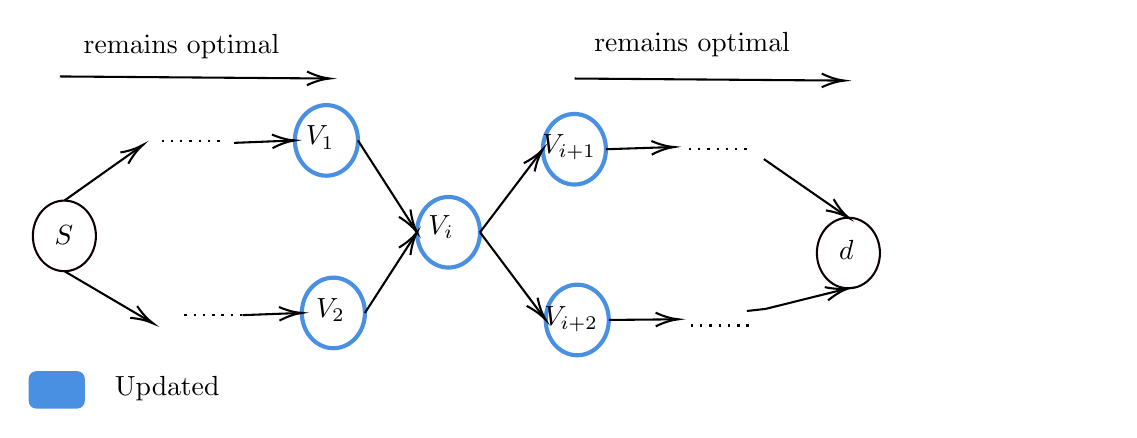
\begin{tikzpicture}[x=0.75pt,y=0.75pt,yscale=-1,xscale=1]
%uncomment if require: \path (0,359); %set diagram left start at 0, and has height of 359

%Shape: Rectangle [id:dp480508071363392] 
\draw  [draw opacity=0][fill={rgb, 255:red, 255; green, 255; blue, 255 }  ,fill opacity=1 ] (572,51) -- (642,51) -- (642,64) -- (572,64) -- cycle ;
%Shape: Rectangle [id:dp03384397152413832] 
\draw  [draw opacity=0][fill={rgb, 255:red, 255; green, 255; blue, 255 }  ,fill opacity=1 ] (573,107) -- (643,107) -- (643,120) -- (573,120) -- cycle ;
%Shape: Ellipse [id:dp9103409908276086] 
\draw  [color={rgb, 255:red, 14; green, 0; blue, 0 }  ,draw opacity=1 ] (125,113.82) .. controls (125,104.43) and (131.8,96.81) .. (140.19,96.81) .. controls (148.57,96.81) and (155.37,104.43) .. (155.37,113.82) .. controls (155.37,123.21) and (148.57,130.82) .. (140.19,130.82) .. controls (131.8,130.82) and (125,123.21) .. (125,113.82) -- cycle ;
%Shape: Ellipse [id:dp740083289005012] 
\draw  [color={rgb, 255:red, 74; green, 144; blue, 226 }  ,draw opacity=1 ][line width=1.5]  (251.25,67.82) .. controls (251.25,58.43) and (258.05,50.81) .. (266.44,50.81) .. controls (274.83,50.81) and (281.63,58.43) .. (281.63,67.82) .. controls (281.63,77.21) and (274.83,84.82) .. (266.44,84.82) .. controls (258.05,84.82) and (251.25,77.21) .. (251.25,67.82) -- cycle ;
%Shape: Ellipse [id:dp9541917593446743] 
\draw  [color={rgb, 255:red, 74; green, 144; blue, 226 }  ,draw opacity=1 ][line width=1.5]  (254.61,150.94) .. controls (254.61,141.55) and (261.41,133.94) .. (269.79,133.94) .. controls (278.18,133.94) and (284.98,141.55) .. (284.98,150.94) .. controls (284.98,160.33) and (278.18,167.94) .. (269.79,167.94) .. controls (261.41,167.94) and (254.61,160.33) .. (254.61,150.94) -- cycle ;
%Shape: Ellipse [id:dp1856273890999922] 
\draw  [color={rgb, 255:red, 74; green, 144; blue, 226 }  ,draw opacity=1 ][line width=1.5]  (310.07,112.07) .. controls (310.07,102.68) and (316.86,95.06) .. (325.25,95.06) .. controls (333.64,95.06) and (340.44,102.68) .. (340.44,112.07) .. controls (340.44,121.46) and (333.64,129.07) .. (325.25,129.07) .. controls (316.86,129.07) and (310.07,121.46) .. (310.07,112.07) -- cycle ;
%Shape: Ellipse [id:dp9526061796743859] 
\draw  [color={rgb, 255:red, 74; green, 144; blue, 226 }  ,draw opacity=1 ][line width=1.5]  (370.73,72.07) .. controls (370.73,62.68) and (377.53,55.06) .. (385.91,55.06) .. controls (394.3,55.06) and (401.1,62.68) .. (401.1,72.07) .. controls (401.1,81.46) and (394.3,89.07) .. (385.91,89.07) .. controls (377.53,89.07) and (370.73,81.46) .. (370.73,72.07) -- cycle ;
%Shape: Ellipse [id:dp044156064147011787] 
\draw  [color={rgb, 255:red, 14; green, 0; blue, 0 }  ,draw opacity=1 ] (502.74,122.07) .. controls (502.74,112.68) and (509.54,105.06) .. (517.93,105.06) .. controls (526.32,105.06) and (533.11,112.68) .. (533.11,122.07) .. controls (533.11,131.46) and (526.32,139.07) .. (517.93,139.07) .. controls (509.54,139.07) and (502.74,131.46) .. (502.74,122.07) -- cycle ;
%Shape: Ellipse [id:dp6843056607618183] 
\draw  [color={rgb, 255:red, 74; green, 144; blue, 226 }  ,draw opacity=1 ][line width=1.5]  (372.1,154.32) .. controls (372.1,144.93) and (378.9,137.32) .. (387.28,137.32) .. controls (395.67,137.32) and (402.47,144.93) .. (402.47,154.32) .. controls (402.47,163.71) and (395.67,171.33) .. (387.28,171.33) .. controls (378.9,171.33) and (372.1,163.71) .. (372.1,154.32) -- cycle ;
%Straight Lines [id:da4109082321511348] 
\draw    (140.19,130.82) -- (181.28,154.99) ;
\draw [shift={(183,156)}, rotate = 210.46] [color={rgb, 255:red, 0; green, 0; blue, 0 }  ][line width=0.75]    (10.93,-3.29) .. controls (6.95,-1.4) and (3.31,-0.3) .. (0,0) .. controls (3.31,0.3) and (6.95,1.4) .. (10.93,3.29)   ;
%Straight Lines [id:da09020512135141656] 
\draw    (140.19,96.81) -- (176.37,71.16) ;
\draw [shift={(178,70)}, rotate = 144.66] [color={rgb, 255:red, 0; green, 0; blue, 0 }  ][line width=0.75]    (10.93,-3.29) .. controls (6.95,-1.4) and (3.31,-0.3) .. (0,0) .. controls (3.31,0.3) and (6.95,1.4) .. (10.93,3.29)   ;
%Straight Lines [id:da07010447777978679] 
\draw    (469,150) -- (478,149) -- (515.99,139.55) ;
\draw [shift={(517.93,139.07)}, rotate = 166.03] [color={rgb, 255:red, 0; green, 0; blue, 0 }  ][line width=0.75]    (10.93,-3.29) .. controls (6.95,-1.4) and (3.31,-0.3) .. (0,0) .. controls (3.31,0.3) and (6.95,1.4) .. (10.93,3.29)   ;
%Straight Lines [id:da3901833128352341] 
\draw    (477.19,76.81) -- (516.28,103.92) ;
\draw [shift={(517.93,105.06)}, rotate = 214.74] [color={rgb, 255:red, 0; green, 0; blue, 0 }  ][line width=0.75]    (10.93,-3.29) .. controls (6.95,-1.4) and (3.31,-0.3) .. (0,0) .. controls (3.31,0.3) and (6.95,1.4) .. (10.93,3.29)   ;
%Straight Lines [id:da5860775319064822] 
\draw    (222,69) -- (249.26,67.9) ;
\draw [shift={(251.25,67.82)}, rotate = 177.68] [color={rgb, 255:red, 0; green, 0; blue, 0 }  ][line width=0.75]    (10.93,-3.29) .. controls (6.95,-1.4) and (3.31,-0.3) .. (0,0) .. controls (3.31,0.3) and (6.95,1.4) .. (10.93,3.29)   ;
%Straight Lines [id:da9472064018730602] 
\draw    (226,152) -- (252.61,151.01) ;
\draw [shift={(254.61,150.94)}, rotate = 177.88] [color={rgb, 255:red, 0; green, 0; blue, 0 }  ][line width=0.75]    (10.93,-3.29) .. controls (6.95,-1.4) and (3.31,-0.3) .. (0,0) .. controls (3.31,0.3) and (6.95,1.4) .. (10.93,3.29)   ;
%Straight Lines [id:da6786123019459969] 
\draw    (281.63,67.82) -- (308.98,110.38) ;
\draw [shift={(310.07,112.07)}, rotate = 237.27] [color={rgb, 255:red, 0; green, 0; blue, 0 }  ][line width=0.75]    (10.93,-3.29) .. controls (6.95,-1.4) and (3.31,-0.3) .. (0,0) .. controls (3.31,0.3) and (6.95,1.4) .. (10.93,3.29)   ;
%Straight Lines [id:da8151696040712353] 
\draw    (284.98,150.94) -- (308.98,113.75) ;
\draw [shift={(310.07,112.07)}, rotate = 122.83] [color={rgb, 255:red, 0; green, 0; blue, 0 }  ][line width=0.75]    (10.93,-3.29) .. controls (6.95,-1.4) and (3.31,-0.3) .. (0,0) .. controls (3.31,0.3) and (6.95,1.4) .. (10.93,3.29)   ;
%Straight Lines [id:da11134508242076424] 
\draw    (340.44,112.07) -- (369.52,73.66) ;
\draw [shift={(370.73,72.07)}, rotate = 127.13] [color={rgb, 255:red, 0; green, 0; blue, 0 }  ][line width=0.75]    (10.93,-3.29) .. controls (6.95,-1.4) and (3.31,-0.3) .. (0,0) .. controls (3.31,0.3) and (6.95,1.4) .. (10.93,3.29)   ;
%Straight Lines [id:da49946303299867534] 
\draw    (340.44,112.07) -- (370.9,152.72) ;
\draw [shift={(372.1,154.32)}, rotate = 233.16] [color={rgb, 255:red, 0; green, 0; blue, 0 }  ][line width=0.75]    (10.93,-3.29) .. controls (6.95,-1.4) and (3.31,-0.3) .. (0,0) .. controls (3.31,0.3) and (6.95,1.4) .. (10.93,3.29)   ;
%Straight Lines [id:da9661195791648898] 
\draw    (401.1,72.07) -- (432,71.06) ;
\draw [shift={(434,71)}, rotate = 178.14] [color={rgb, 255:red, 0; green, 0; blue, 0 }  ][line width=0.75]    (10.93,-3.29) .. controls (6.95,-1.4) and (3.31,-0.3) .. (0,0) .. controls (3.31,0.3) and (6.95,1.4) .. (10.93,3.29)   ;
%Straight Lines [id:da9084929098821986] 
\draw    (402.47,154.32) -- (434,154.02) ;
\draw [shift={(436,154)}, rotate = 179.45] [color={rgb, 255:red, 0; green, 0; blue, 0 }  ][line width=0.75]    (10.93,-3.29) .. controls (6.95,-1.4) and (3.31,-0.3) .. (0,0) .. controls (3.31,0.3) and (6.95,1.4) .. (10.93,3.29)   ;
%Straight Lines [id:da0449100159502247] 
\draw  [dash pattern={on 0.84pt off 2.51pt}]  (187,68) -- (215,68) ;
%Straight Lines [id:da5356080041931417] 
\draw  [dash pattern={on 0.84pt off 2.51pt}]  (198,152) -- (226,152) ;
%Straight Lines [id:da9346868766060579] 
\draw  [dash pattern={on 0.84pt off 2.51pt}]  (441,72) -- (469,72) ;
%Straight Lines [id:da9642012858007416] 
\draw  [dash pattern={on 0.84pt off 2.51pt}]  (442,157) -- (470,157) ;
%Rounded Rect [id:dp6788726220855428] 
\draw  [draw opacity=0][fill={rgb, 255:red, 74; green, 144; blue, 226 }  ,fill opacity=1 ] (123,182.6) .. controls (123,180.61) and (124.61,179) .. (126.6,179) -- (146.4,179) .. controls (148.39,179) and (150,180.61) .. (150,182.6) -- (150,193.4) .. controls (150,195.39) and (148.39,197) .. (146.4,197) -- (126.6,197) .. controls (124.61,197) and (123,195.39) .. (123,193.4) -- cycle ;
%Straight Lines [id:da6555072227430381] 
\draw    (138,37) -- (266,37.98) ;
\draw [shift={(268,38)}, rotate = 180.44] [color={rgb, 255:red, 0; green, 0; blue, 0 }  ][line width=0.75]    (10.93,-3.29) .. controls (6.95,-1.4) and (3.31,-0.3) .. (0,0) .. controls (3.31,0.3) and (6.95,1.4) .. (10.93,3.29)   ;
%Straight Lines [id:da6809797244968319] 
\draw    (386,38) -- (514,38.98) ;
\draw [shift={(516,39)}, rotate = 180.44] [color={rgb, 255:red, 0; green, 0; blue, 0 }  ][line width=0.75]    (10.93,-3.29) .. controls (6.95,-1.4) and (3.31,-0.3) .. (0,0) .. controls (3.31,0.3) and (6.95,1.4) .. (10.93,3.29)   ;

% Text Node
\draw (134,107.4) node [anchor=north west][inner sep=0.75pt]    {$S$};
% Text Node
\draw (255,59.4) node [anchor=north west][inner sep=0.75pt]    {$V_{1}$};
% Text Node
\draw (260,142.4) node [anchor=north west][inner sep=0.75pt]    {$V_{2}$};
% Text Node
\draw (314,102.4) node [anchor=north west][inner sep=0.75pt]    {$V_{i}$};
% Text Node
\draw (369,63.4) node [anchor=north west][inner sep=0.75pt]    {$V_{i+1}$};
% Text Node
\draw (370,146.4) node [anchor=north west][inner sep=0.75pt]    {$V_{i+2}$};
% Text Node
\draw (512,114.4) node [anchor=north west][inner sep=0.75pt]    {$d$};
% Text Node
\draw (163,180) node [anchor=north west][inner sep=0.75pt]   [align=left] {Updated};
% Text Node
\draw (148,15) node [anchor=north west][inner sep=0.75pt]   [align=left] {remains optimal};
% Text Node
\draw (394,14) node [anchor=north west][inner sep=0.75pt]   [align=left] {remains optimal};


\end{tikzpicture}
    Figure 5: Dynamic update by vertices weights
\end{center}

\textbf{Proposition.} If no weight updates occur to the intersection of the set of fathers / predecessors of $d_j$ and the set of children of $s_i$, then the optimality of $s_i-d_j$ paths are preserved.

\textit{Proof.} Let $\Delta = ((w'(s_i) - w(s_i) + (w'(d_i) - w(d_i))$ be the net weight change of $s_i$ and $d_j$. Then for any path $p_i$, the new weight is $w'(p_i) = w(p_i) + \Delta$. It follows a minimal path weight $p_k$ is preserved. Indeed, if we have real numbers $a_1, a_2, \dots, a_k$ with minimum $a_k$, then $(a_k + \Delta)$ would be a minimum of $(a_1 + \Delta), \dots, (a_k + \Delta)$.

\textbf{Procedure.}
\begin{itemize}
    \item Memoize all pairs in the left subgraph and right subgraph through the previously computed distances and predecessors matrices.
    \item Call any all pairs shortest path algorithm.
\end{itemize}

\begin{verbatim}
# input: matrix updatedGraph, with the newly updated weights
#        list updatedVertices
#        2d list preDistances, the previously computed distances matrix
#        2d list prePredecessors, the previously computed predecessor matrix
def dynamicAllPairsShortestPath(updatedGraph, updatedVertices, preDistances, prePredecessors):
    
    # length
    n = len(updatedGraph)
    
    # initialize empty memoization
    distMemo = {}
    predMemo = {}
    
    # for all pairs
    for i in range(n):
        for j in range(n):
            # left subgraph with no updated vertices
            if i < min(updatedVertices) and j < min(updatedVertices):
            
                # memoize the previously computed distance
                dist_memo[(i,j,n)] = preDistances[i][j]
                
                # memoize the previously computed predecessor
                pred_memo[(i,j,n)] = prePredecessors[i][j]
            
            # right subgraph with no updated vertices
            if i > max(updatedVertices) and j > max(updatedVertices):
            
                # memoize the previously computed distance
                dist_memo[(i,j,n)] = preDistances[i][j]
                
                # memoize the previously computed predecessor
                pred_memo[(i,j,n)] = prePredecessors[i][j]
    
    # execute all pairs shortest path algorithm but without recomputing memoized pairs
    return AllPairsShortestPath(updatedGraph, distMemo, predMemo)
\end{verbatim}

\textbf{Corollary.} Procedure correctness.

\textit{Proof.} We already know the correctness of memoization from the previous \textit{lemma}. Given a correct memoization, the correctness of the all pairs shortest path is given, since it is used as a black-box subroutine. $\blacksquare$


\textbf{Diameter}

\begin{center}
    \tikzset{every picture/.style={line width=0.75pt}} %set default line width to 0.75pt        

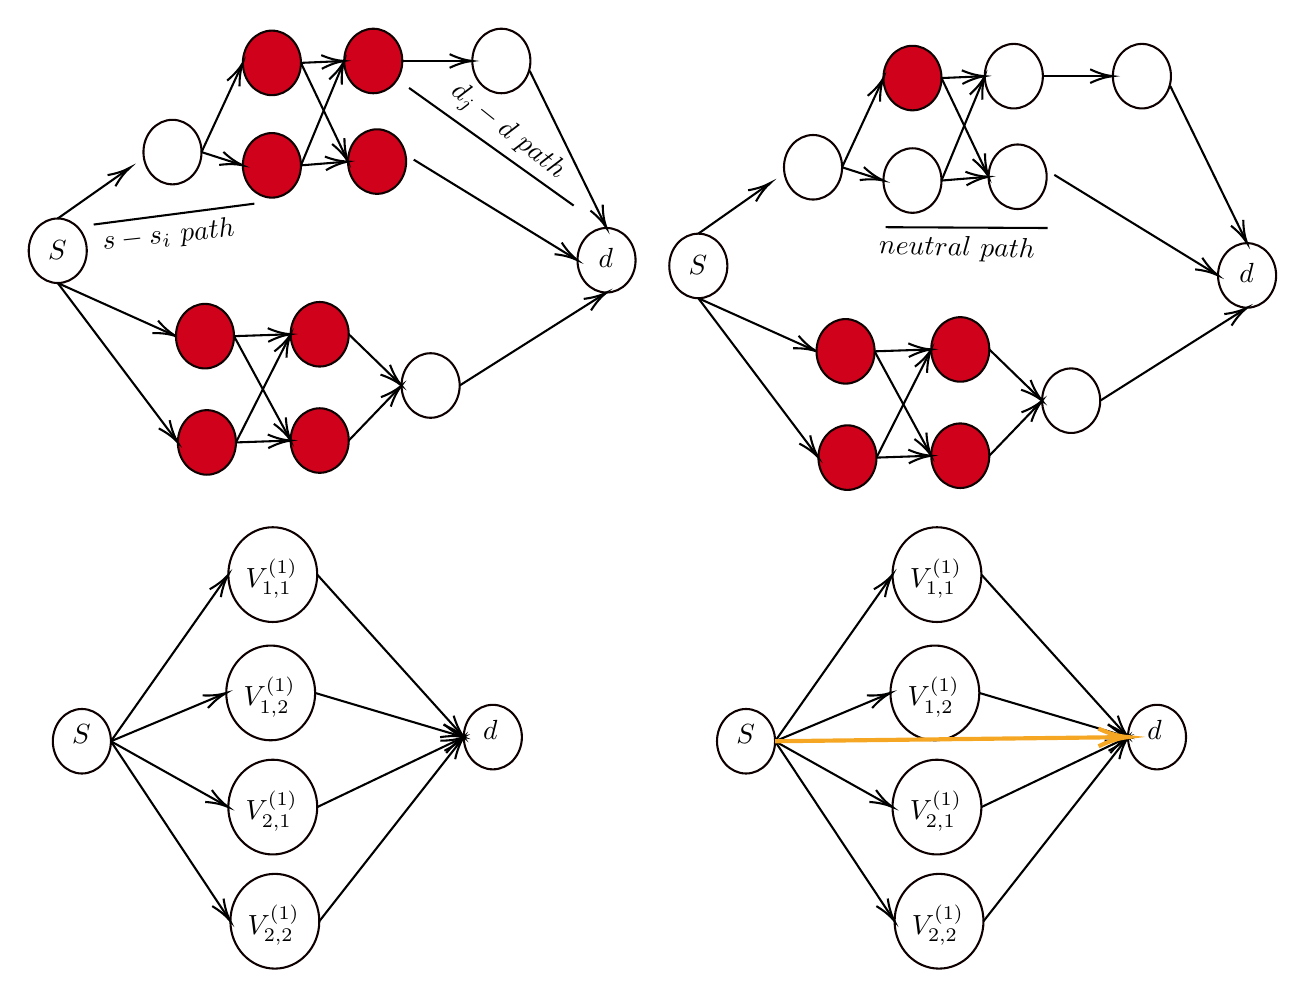
\begin{tikzpicture}[x=0.75pt,y=0.75pt,yscale=-1,xscale=1]
%uncomment if require: \path (0,484); %set diagram left start at 0, and has height of 484

%Shape: Ellipse [id:dp9103409908276086] 
\draw  [color={rgb, 255:red, 14; green, 0; blue, 0 }  ,draw opacity=1 ] (3,117.79) .. controls (3,109.21) and (9.26,102.25) .. (16.99,102.25) .. controls (24.72,102.25) and (30.98,109.21) .. (30.98,117.79) .. controls (30.98,126.38) and (24.72,133.34) .. (16.99,133.34) .. controls (9.26,133.34) and (3,126.38) .. (3,117.79) -- cycle ;
%Straight Lines [id:da4109082321511348] 
\draw    (16.99,133.34) -- (72.11,158.12) ;
\draw [shift={(73.94,158.94)}, rotate = 204.21] [color={rgb, 255:red, 0; green, 0; blue, 0 }  ][line width=0.75]    (10.93,-3.29) .. controls (6.95,-1.4) and (3.31,-0.3) .. (0,0) .. controls (3.31,0.3) and (6.95,1.4) .. (10.93,3.29)   ;
%Straight Lines [id:da09020512135141656] 
\draw    (16.99,102.25) -- (50.19,78.88) ;
\draw [shift={(51.83,77.73)}, rotate = 144.86] [color={rgb, 255:red, 0; green, 0; blue, 0 }  ][line width=0.75]    (10.93,-3.29) .. controls (6.95,-1.4) and (3.31,-0.3) .. (0,0) .. controls (3.31,0.3) and (6.95,1.4) .. (10.93,3.29)   ;
%Shape: Ellipse [id:dp8555391049060532] 
\draw  [color={rgb, 255:red, 14; green, 0; blue, 0 }  ,draw opacity=1 ] (58.28,70.25) .. controls (58.28,61.66) and (64.54,54.7) .. (72.27,54.7) .. controls (79.99,54.7) and (86.26,61.66) .. (86.26,70.25) .. controls (86.26,78.83) and (79.99,85.79) .. (72.27,85.79) .. controls (64.54,85.79) and (58.28,78.83) .. (58.28,70.25) -- cycle ;
%Shape: Ellipse [id:dp883776495100441] 
\draw  [color={rgb, 255:red, 14; green, 0; blue, 0 }  ,draw opacity=1 ][fill={rgb, 255:red, 208; green, 2; blue, 27 }  ,fill opacity=1 ] (73.94,158.94) .. controls (73.94,150.35) and (80.2,143.39) .. (87.93,143.39) .. controls (95.65,143.39) and (101.92,150.35) .. (101.92,158.94) .. controls (101.92,167.52) and (95.65,174.48) .. (87.93,174.48) .. controls (80.2,174.48) and (73.94,167.52) .. (73.94,158.94) -- cycle ;
%Shape: Ellipse [id:dp0013391091782246622] 
\draw  [color={rgb, 255:red, 14; green, 0; blue, 0 }  ,draw opacity=1 ][fill={rgb, 255:red, 208; green, 2; blue, 27 }  ,fill opacity=1 ] (129.21,158.02) .. controls (129.21,149.44) and (135.48,142.48) .. (143.2,142.48) .. controls (150.93,142.48) and (157.19,149.44) .. (157.19,158.02) .. controls (157.19,166.61) and (150.93,173.57) .. (143.2,173.57) .. controls (135.48,173.57) and (129.21,166.61) .. (129.21,158.02) -- cycle ;
%Shape: Ellipse [id:dp14800055787625244] 
\draw  [color={rgb, 255:red, 14; green, 0; blue, 0 }  ,draw opacity=1 ][fill={rgb, 255:red, 208; green, 2; blue, 27 }  ,fill opacity=1 ] (74.86,210.14) .. controls (74.86,201.55) and (81.12,194.59) .. (88.85,194.59) .. controls (96.57,194.59) and (102.84,201.55) .. (102.84,210.14) .. controls (102.84,218.73) and (96.57,225.69) .. (88.85,225.69) .. controls (81.12,225.69) and (74.86,218.73) .. (74.86,210.14) -- cycle ;
%Shape: Ellipse [id:dp6447783194707915] 
\draw  [color={rgb, 255:red, 14; green, 0; blue, 0 }  ,draw opacity=1 ][fill={rgb, 255:red, 208; green, 2; blue, 27 }  ,fill opacity=1 ] (129.21,209.23) .. controls (129.21,200.64) and (135.48,193.68) .. (143.2,193.68) .. controls (150.93,193.68) and (157.19,200.64) .. (157.19,209.23) .. controls (157.19,217.81) and (150.93,224.77) .. (143.2,224.77) .. controls (135.48,224.77) and (129.21,217.81) .. (129.21,209.23) -- cycle ;
%Straight Lines [id:da27074959809886323] 
\draw    (16.99,133.34) -- (73.65,208.54) ;
\draw [shift={(74.86,210.14)}, rotate = 233] [color={rgb, 255:red, 0; green, 0; blue, 0 }  ][line width=0.75]    (10.93,-3.29) .. controls (6.95,-1.4) and (3.31,-0.3) .. (0,0) .. controls (3.31,0.3) and (6.95,1.4) .. (10.93,3.29)   ;
%Straight Lines [id:da4655911040283116] 
\draw    (101.92,158.94) -- (127.21,158.09) ;
\draw [shift={(129.21,158.02)}, rotate = 178.08] [color={rgb, 255:red, 0; green, 0; blue, 0 }  ][line width=0.75]    (10.93,-3.29) .. controls (6.95,-1.4) and (3.31,-0.3) .. (0,0) .. controls (3.31,0.3) and (6.95,1.4) .. (10.93,3.29)   ;
%Straight Lines [id:da9192059110695721] 
\draw    (101.92,158.94) -- (128.26,207.47) ;
\draw [shift={(129.21,209.23)}, rotate = 241.51] [color={rgb, 255:red, 0; green, 0; blue, 0 }  ][line width=0.75]    (10.93,-3.29) .. controls (6.95,-1.4) and (3.31,-0.3) .. (0,0) .. controls (3.31,0.3) and (6.95,1.4) .. (10.93,3.29)   ;
%Straight Lines [id:da9848706499509929] 
\draw    (102.84,210.14) -- (128.31,159.81) ;
\draw [shift={(129.21,158.02)}, rotate = 116.84] [color={rgb, 255:red, 0; green, 0; blue, 0 }  ][line width=0.75]    (10.93,-3.29) .. controls (6.95,-1.4) and (3.31,-0.3) .. (0,0) .. controls (3.31,0.3) and (6.95,1.4) .. (10.93,3.29)   ;
%Straight Lines [id:da19173855653949] 
\draw    (102.84,210.14) -- (127.21,209.29) ;
\draw [shift={(129.21,209.23)}, rotate = 178.01] [color={rgb, 255:red, 0; green, 0; blue, 0 }  ][line width=0.75]    (10.93,-3.29) .. controls (6.95,-1.4) and (3.31,-0.3) .. (0,0) .. controls (3.31,0.3) and (6.95,1.4) .. (10.93,3.29)   ;
%Shape: Ellipse [id:dp7994013969403357] 
\draw  [color={rgb, 255:red, 14; green, 0; blue, 0 }  ,draw opacity=1 ] (182.64,182.71) .. controls (182.64,174.12) and (188.91,167.16) .. (196.63,167.16) .. controls (204.36,167.16) and (210.63,174.12) .. (210.63,182.71) .. controls (210.63,191.3) and (204.36,198.26) .. (196.63,198.26) .. controls (188.91,198.26) and (182.64,191.3) .. (182.64,182.71) -- cycle ;
%Straight Lines [id:da827830318999168] 
\draw    (157.19,158.02) -- (181.21,181.32) ;
\draw [shift={(182.64,182.71)}, rotate = 224.13] [color={rgb, 255:red, 0; green, 0; blue, 0 }  ][line width=0.75]    (10.93,-3.29) .. controls (6.95,-1.4) and (3.31,-0.3) .. (0,0) .. controls (3.31,0.3) and (6.95,1.4) .. (10.93,3.29)   ;
%Straight Lines [id:da40645669775739135] 
\draw    (157.19,209.23) -- (181.26,184.15) ;
\draw [shift={(182.64,182.71)}, rotate = 133.83] [color={rgb, 255:red, 0; green, 0; blue, 0 }  ][line width=0.75]    (10.93,-3.29) .. controls (6.95,-1.4) and (3.31,-0.3) .. (0,0) .. controls (3.31,0.3) and (6.95,1.4) .. (10.93,3.29)   ;
%Shape: Ellipse [id:dp6103012107886219] 
\draw  [color={rgb, 255:red, 14; green, 0; blue, 0 }  ,draw opacity=1 ] (267.4,122.36) .. controls (267.4,113.78) and (273.66,106.82) .. (281.39,106.82) .. controls (289.12,106.82) and (295.38,113.78) .. (295.38,122.36) .. controls (295.38,130.95) and (289.12,137.91) .. (281.39,137.91) .. controls (273.66,137.91) and (267.4,130.95) .. (267.4,122.36) -- cycle ;
%Straight Lines [id:da2986672943287987] 
\draw    (210.63,182.71) -- (279.7,138.98) ;
\draw [shift={(281.39,137.91)}, rotate = 147.66] [color={rgb, 255:red, 0; green, 0; blue, 0 }  ][line width=0.75]    (10.93,-3.29) .. controls (6.95,-1.4) and (3.31,-0.3) .. (0,0) .. controls (3.31,0.3) and (6.95,1.4) .. (10.93,3.29)   ;
%Shape: Ellipse [id:dp6623747127336961] 
\draw  [color={rgb, 255:red, 14; green, 0; blue, 0 }  ,draw opacity=1 ][fill={rgb, 255:red, 208; green, 2; blue, 27 }  ,fill opacity=1 ] (106.18,27.27) .. controls (106.18,18.69) and (112.44,11.73) .. (120.17,11.73) .. controls (127.9,11.73) and (134.16,18.69) .. (134.16,27.27) .. controls (134.16,35.86) and (127.9,42.82) .. (120.17,42.82) .. controls (112.44,42.82) and (106.18,35.86) .. (106.18,27.27) -- cycle ;
%Shape: Ellipse [id:dp568381457733701] 
\draw  [color={rgb, 255:red, 14; green, 0; blue, 0 }  ,draw opacity=1 ][fill={rgb, 255:red, 208; green, 2; blue, 27 }  ,fill opacity=1 ] (106.18,76.65) .. controls (106.18,68.06) and (112.44,61.1) .. (120.17,61.1) .. controls (127.9,61.1) and (134.16,68.06) .. (134.16,76.65) .. controls (134.16,85.23) and (127.9,92.19) .. (120.17,92.19) .. controls (112.44,92.19) and (106.18,85.23) .. (106.18,76.65) -- cycle ;
%Shape: Ellipse [id:dp23960485909454166] 
\draw  [color={rgb, 255:red, 14; green, 0; blue, 0 }  ,draw opacity=1 ][fill={rgb, 255:red, 208; green, 2; blue, 27 }  ,fill opacity=1 ] (155.01,26.36) .. controls (155.01,17.77) and (161.27,10.81) .. (169,10.81) .. controls (176.72,10.81) and (182.99,17.77) .. (182.99,26.36) .. controls (182.99,34.94) and (176.72,41.9) .. (169,41.9) .. controls (161.27,41.9) and (155.01,34.94) .. (155.01,26.36) -- cycle ;
%Shape: Ellipse [id:dp03538565261265392] 
\draw  [color={rgb, 255:red, 14; green, 0; blue, 0 }  ,draw opacity=1 ][fill={rgb, 255:red, 208; green, 2; blue, 27 }  ,fill opacity=1 ] (156.85,74.82) .. controls (156.85,66.23) and (163.11,59.27) .. (170.84,59.27) .. controls (178.57,59.27) and (184.83,66.23) .. (184.83,74.82) .. controls (184.83,83.4) and (178.57,90.36) .. (170.84,90.36) .. controls (163.11,90.36) and (156.85,83.4) .. (156.85,74.82) -- cycle ;
%Shape: Ellipse [id:dp11156840512064159] 
\draw  [color={rgb, 255:red, 14; green, 0; blue, 0 }  ,draw opacity=1 ] (216.73,26.36) .. controls (216.73,17.77) and (222.99,10.81) .. (230.72,10.81) .. controls (238.45,10.81) and (244.71,17.77) .. (244.71,26.36) .. controls (244.71,34.94) and (238.45,41.9) .. (230.72,41.9) .. controls (222.99,41.9) and (216.73,34.94) .. (216.73,26.36) -- cycle ;
%Straight Lines [id:da15333951029025084] 
\draw    (244.37,31.1) -- (280.51,105.02) ;
\draw [shift={(281.39,106.82)}, rotate = 243.94] [color={rgb, 255:red, 0; green, 0; blue, 0 }  ][line width=0.75]    (10.93,-3.29) .. controls (6.95,-1.4) and (3.31,-0.3) .. (0,0) .. controls (3.31,0.3) and (6.95,1.4) .. (10.93,3.29)   ;
%Straight Lines [id:da3002385569603043] 
\draw    (182.99,26.36) -- (214.73,26.36) ;
\draw [shift={(216.73,26.36)}, rotate = 180] [color={rgb, 255:red, 0; green, 0; blue, 0 }  ][line width=0.75]    (10.93,-3.29) .. controls (6.95,-1.4) and (3.31,-0.3) .. (0,0) .. controls (3.31,0.3) and (6.95,1.4) .. (10.93,3.29)   ;
%Straight Lines [id:da7951506053416368] 
\draw    (188.51,73.9) -- (265.7,121.32) ;
\draw [shift={(267.4,122.36)}, rotate = 211.56] [color={rgb, 255:red, 0; green, 0; blue, 0 }  ][line width=0.75]    (10.93,-3.29) .. controls (6.95,-1.4) and (3.31,-0.3) .. (0,0) .. controls (3.31,0.3) and (6.95,1.4) .. (10.93,3.29)   ;
%Straight Lines [id:da7041644417397548] 
\draw    (86.26,70.25) -- (105.34,29.09) ;
\draw [shift={(106.18,27.27)}, rotate = 114.87] [color={rgb, 255:red, 0; green, 0; blue, 0 }  ][line width=0.75]    (10.93,-3.29) .. controls (6.95,-1.4) and (3.31,-0.3) .. (0,0) .. controls (3.31,0.3) and (6.95,1.4) .. (10.93,3.29)   ;
%Straight Lines [id:da19456235099965924] 
\draw    (86.26,70.25) -- (104.28,76.04) ;
\draw [shift={(106.18,76.65)}, rotate = 197.81] [color={rgb, 255:red, 0; green, 0; blue, 0 }  ][line width=0.75]    (10.93,-3.29) .. controls (6.95,-1.4) and (3.31,-0.3) .. (0,0) .. controls (3.31,0.3) and (6.95,1.4) .. (10.93,3.29)   ;
%Straight Lines [id:da6137491537973168] 
\draw    (134.16,27.27) -- (153.01,26.45) ;
\draw [shift={(155.01,26.36)}, rotate = 177.49] [color={rgb, 255:red, 0; green, 0; blue, 0 }  ][line width=0.75]    (10.93,-3.29) .. controls (6.95,-1.4) and (3.31,-0.3) .. (0,0) .. controls (3.31,0.3) and (6.95,1.4) .. (10.93,3.29)   ;
%Straight Lines [id:da3222854329811604] 
\draw    (134.16,27.27) -- (155.99,73.01) ;
\draw [shift={(156.85,74.82)}, rotate = 244.49] [color={rgb, 255:red, 0; green, 0; blue, 0 }  ][line width=0.75]    (10.93,-3.29) .. controls (6.95,-1.4) and (3.31,-0.3) .. (0,0) .. controls (3.31,0.3) and (6.95,1.4) .. (10.93,3.29)   ;
%Straight Lines [id:da6170165558479803] 
\draw    (134.16,76.65) -- (154.24,28.21) ;
\draw [shift={(155.01,26.36)}, rotate = 112.52] [color={rgb, 255:red, 0; green, 0; blue, 0 }  ][line width=0.75]    (10.93,-3.29) .. controls (6.95,-1.4) and (3.31,-0.3) .. (0,0) .. controls (3.31,0.3) and (6.95,1.4) .. (10.93,3.29)   ;
%Straight Lines [id:da12935379402032376] 
\draw    (134.16,76.65) -- (154.86,74.98) ;
\draw [shift={(156.85,74.82)}, rotate = 175.39] [color={rgb, 255:red, 0; green, 0; blue, 0 }  ][line width=0.75]    (10.93,-3.29) .. controls (6.95,-1.4) and (3.31,-0.3) .. (0,0) .. controls (3.31,0.3) and (6.95,1.4) .. (10.93,3.29)   ;
%Straight Lines [id:da6131121743340329] 
\draw    (34.32,105.16) -- (111.71,95.1) ;
%Straight Lines [id:da65257178024222] 
\draw    (186.26,39.35) -- (265.56,96.02) ;
%Shape: Ellipse [id:dp3324632249793371] 
\draw  [color={rgb, 255:red, 14; green, 0; blue, 0 }  ,draw opacity=1 ] (311.62,125.11) .. controls (311.62,116.52) and (317.88,109.56) .. (325.61,109.56) .. controls (333.34,109.56) and (339.6,116.52) .. (339.6,125.11) .. controls (339.6,133.69) and (333.34,140.65) .. (325.61,140.65) .. controls (317.88,140.65) and (311.62,133.69) .. (311.62,125.11) -- cycle ;
%Straight Lines [id:da8426027772818339] 
\draw    (325.61,140.65) -- (380.73,165.43) ;
\draw [shift={(382.56,166.25)}, rotate = 204.21] [color={rgb, 255:red, 0; green, 0; blue, 0 }  ][line width=0.75]    (10.93,-3.29) .. controls (6.95,-1.4) and (3.31,-0.3) .. (0,0) .. controls (3.31,0.3) and (6.95,1.4) .. (10.93,3.29)   ;
%Straight Lines [id:da7627219268640635] 
\draw    (325.61,109.56) -- (358.81,86.2) ;
\draw [shift={(360.45,85.04)}, rotate = 144.86] [color={rgb, 255:red, 0; green, 0; blue, 0 }  ][line width=0.75]    (10.93,-3.29) .. controls (6.95,-1.4) and (3.31,-0.3) .. (0,0) .. controls (3.31,0.3) and (6.95,1.4) .. (10.93,3.29)   ;
%Shape: Ellipse [id:dp10195816258153978] 
\draw  [color={rgb, 255:red, 14; green, 0; blue, 0 }  ,draw opacity=1 ] (366.89,77.56) .. controls (366.89,68.98) and (373.16,62.02) .. (380.89,62.02) .. controls (388.61,62.02) and (394.88,68.98) .. (394.88,77.56) .. controls (394.88,86.15) and (388.61,93.11) .. (380.89,93.11) .. controls (373.16,93.11) and (366.89,86.15) .. (366.89,77.56) -- cycle ;
%Shape: Ellipse [id:dp5022300899911052] 
\draw  [color={rgb, 255:red, 14; green, 0; blue, 0 }  ,draw opacity=1 ][fill={rgb, 255:red, 208; green, 2; blue, 27 }  ,fill opacity=1 ] (382.56,166.25) .. controls (382.56,157.67) and (388.82,150.71) .. (396.55,150.71) .. controls (404.27,150.71) and (410.54,157.67) .. (410.54,166.25) .. controls (410.54,174.84) and (404.27,181.8) .. (396.55,181.8) .. controls (388.82,181.8) and (382.56,174.84) .. (382.56,166.25) -- cycle ;
%Shape: Ellipse [id:dp17677518343162024] 
\draw  [color={rgb, 255:red, 14; green, 0; blue, 0 }  ,draw opacity=1 ][fill={rgb, 255:red, 208; green, 2; blue, 27 }  ,fill opacity=1 ] (437.83,165.34) .. controls (437.83,156.75) and (444.1,149.79) .. (451.82,149.79) .. controls (459.55,149.79) and (465.81,156.75) .. (465.81,165.34) .. controls (465.81,173.92) and (459.55,180.88) .. (451.82,180.88) .. controls (444.1,180.88) and (437.83,173.92) .. (437.83,165.34) -- cycle ;
%Shape: Ellipse [id:dp7924693110618928] 
\draw  [color={rgb, 255:red, 14; green, 0; blue, 0 }  ,draw opacity=1 ][fill={rgb, 255:red, 208; green, 2; blue, 27 }  ,fill opacity=1 ] (383.48,217.45) .. controls (383.48,208.87) and (389.74,201.91) .. (397.47,201.91) .. controls (405.19,201.91) and (411.46,208.87) .. (411.46,217.45) .. controls (411.46,226.04) and (405.19,233) .. (397.47,233) .. controls (389.74,233) and (383.48,226.04) .. (383.48,217.45) -- cycle ;
%Shape: Ellipse [id:dp6605698235890625] 
\draw  [color={rgb, 255:red, 14; green, 0; blue, 0 }  ,draw opacity=1 ][fill={rgb, 255:red, 208; green, 2; blue, 27 }  ,fill opacity=1 ] (437.83,216.54) .. controls (437.83,207.95) and (444.1,200.99) .. (451.82,200.99) .. controls (459.55,200.99) and (465.81,207.95) .. (465.81,216.54) .. controls (465.81,225.13) and (459.55,232.09) .. (451.82,232.09) .. controls (444.1,232.09) and (437.83,225.13) .. (437.83,216.54) -- cycle ;
%Straight Lines [id:da9499427754983338] 
\draw    (325.61,140.65) -- (382.27,215.86) ;
\draw [shift={(383.48,217.45)}, rotate = 233] [color={rgb, 255:red, 0; green, 0; blue, 0 }  ][line width=0.75]    (10.93,-3.29) .. controls (6.95,-1.4) and (3.31,-0.3) .. (0,0) .. controls (3.31,0.3) and (6.95,1.4) .. (10.93,3.29)   ;
%Straight Lines [id:da3682039996908384] 
\draw    (410.54,166.25) -- (435.83,165.4) ;
\draw [shift={(437.83,165.34)}, rotate = 178.08] [color={rgb, 255:red, 0; green, 0; blue, 0 }  ][line width=0.75]    (10.93,-3.29) .. controls (6.95,-1.4) and (3.31,-0.3) .. (0,0) .. controls (3.31,0.3) and (6.95,1.4) .. (10.93,3.29)   ;
%Straight Lines [id:da575001507238937] 
\draw    (410.54,166.25) -- (436.88,214.78) ;
\draw [shift={(437.83,216.54)}, rotate = 241.51] [color={rgb, 255:red, 0; green, 0; blue, 0 }  ][line width=0.75]    (10.93,-3.29) .. controls (6.95,-1.4) and (3.31,-0.3) .. (0,0) .. controls (3.31,0.3) and (6.95,1.4) .. (10.93,3.29)   ;
%Straight Lines [id:da7707372942218098] 
\draw    (411.46,217.45) -- (436.93,167.12) ;
\draw [shift={(437.83,165.34)}, rotate = 116.84] [color={rgb, 255:red, 0; green, 0; blue, 0 }  ][line width=0.75]    (10.93,-3.29) .. controls (6.95,-1.4) and (3.31,-0.3) .. (0,0) .. controls (3.31,0.3) and (6.95,1.4) .. (10.93,3.29)   ;
%Straight Lines [id:da7047899822090402] 
\draw    (411.46,217.45) -- (435.83,216.61) ;
\draw [shift={(437.83,216.54)}, rotate = 178.01] [color={rgb, 255:red, 0; green, 0; blue, 0 }  ][line width=0.75]    (10.93,-3.29) .. controls (6.95,-1.4) and (3.31,-0.3) .. (0,0) .. controls (3.31,0.3) and (6.95,1.4) .. (10.93,3.29)   ;
%Shape: Ellipse [id:dp2381911640263179] 
\draw  [color={rgb, 255:red, 14; green, 0; blue, 0 }  ,draw opacity=1 ] (491.26,190.02) .. controls (491.26,181.44) and (497.53,174.48) .. (505.25,174.48) .. controls (512.98,174.48) and (519.24,181.44) .. (519.24,190.02) .. controls (519.24,198.61) and (512.98,205.57) .. (505.25,205.57) .. controls (497.53,205.57) and (491.26,198.61) .. (491.26,190.02) -- cycle ;
%Straight Lines [id:da2774736655988086] 
\draw    (465.81,165.34) -- (489.83,188.63) ;
\draw [shift={(491.26,190.02)}, rotate = 224.13] [color={rgb, 255:red, 0; green, 0; blue, 0 }  ][line width=0.75]    (10.93,-3.29) .. controls (6.95,-1.4) and (3.31,-0.3) .. (0,0) .. controls (3.31,0.3) and (6.95,1.4) .. (10.93,3.29)   ;
%Straight Lines [id:da04763370368731046] 
\draw    (465.81,216.54) -- (489.88,191.47) ;
\draw [shift={(491.26,190.02)}, rotate = 133.83] [color={rgb, 255:red, 0; green, 0; blue, 0 }  ][line width=0.75]    (10.93,-3.29) .. controls (6.95,-1.4) and (3.31,-0.3) .. (0,0) .. controls (3.31,0.3) and (6.95,1.4) .. (10.93,3.29)   ;
%Shape: Ellipse [id:dp08932201466234568] 
\draw  [color={rgb, 255:red, 14; green, 0; blue, 0 }  ,draw opacity=1 ] (576.02,129.68) .. controls (576.02,121.09) and (582.28,114.13) .. (590.01,114.13) .. controls (597.74,114.13) and (604,121.09) .. (604,129.68) .. controls (604,138.26) and (597.74,145.22) .. (590.01,145.22) .. controls (582.28,145.22) and (576.02,138.26) .. (576.02,129.68) -- cycle ;
%Straight Lines [id:da6939700447337489] 
\draw    (519.24,190.02) -- (588.32,146.29) ;
\draw [shift={(590.01,145.22)}, rotate = 147.66] [color={rgb, 255:red, 0; green, 0; blue, 0 }  ][line width=0.75]    (10.93,-3.29) .. controls (6.95,-1.4) and (3.31,-0.3) .. (0,0) .. controls (3.31,0.3) and (6.95,1.4) .. (10.93,3.29)   ;
%Shape: Ellipse [id:dp6322922737607573] 
\draw  [color={rgb, 255:red, 14; green, 0; blue, 0 }  ,draw opacity=1 ][fill={rgb, 255:red, 208; green, 2; blue, 27 }  ,fill opacity=1 ] (414.8,34.59) .. controls (414.8,26) and (421.06,19.04) .. (428.79,19.04) .. controls (436.52,19.04) and (442.78,26) .. (442.78,34.59) .. controls (442.78,43.17) and (436.52,50.13) .. (428.79,50.13) .. controls (421.06,50.13) and (414.8,43.17) .. (414.8,34.59) -- cycle ;
%Shape: Ellipse [id:dp11052346799739121] 
\draw  [color={rgb, 255:red, 14; green, 0; blue, 0 }  ,draw opacity=1 ] (414.8,83.96) .. controls (414.8,75.38) and (421.06,68.42) .. (428.79,68.42) .. controls (436.52,68.42) and (442.78,75.38) .. (442.78,83.96) .. controls (442.78,92.55) and (436.52,99.51) .. (428.79,99.51) .. controls (421.06,99.51) and (414.8,92.55) .. (414.8,83.96) -- cycle ;
%Shape: Ellipse [id:dp17081434567182852] 
\draw  [color={rgb, 255:red, 14; green, 0; blue, 0 }  ,draw opacity=1 ] (463.63,33.67) .. controls (463.63,25.09) and (469.89,18.13) .. (477.62,18.13) .. controls (485.34,18.13) and (491.61,25.09) .. (491.61,33.67) .. controls (491.61,42.26) and (485.34,49.22) .. (477.62,49.22) .. controls (469.89,49.22) and (463.63,42.26) .. (463.63,33.67) -- cycle ;
%Shape: Ellipse [id:dp1228438804456613] 
\draw  [color={rgb, 255:red, 14; green, 0; blue, 0 }  ,draw opacity=1 ] (465.47,82.13) .. controls (465.47,73.55) and (471.73,66.59) .. (479.46,66.59) .. controls (487.19,66.59) and (493.45,73.55) .. (493.45,82.13) .. controls (493.45,90.72) and (487.19,97.68) .. (479.46,97.68) .. controls (471.73,97.68) and (465.47,90.72) .. (465.47,82.13) -- cycle ;
%Shape: Ellipse [id:dp9474923341878037] 
\draw  [color={rgb, 255:red, 14; green, 0; blue, 0 }  ,draw opacity=1 ] (525.35,33.67) .. controls (525.35,25.09) and (531.61,18.13) .. (539.34,18.13) .. controls (547.07,18.13) and (553.33,25.09) .. (553.33,33.67) .. controls (553.33,42.26) and (547.07,49.22) .. (539.34,49.22) .. controls (531.61,49.22) and (525.35,42.26) .. (525.35,33.67) -- cycle ;
%Straight Lines [id:da2377260705243509] 
\draw    (552.99,38.41) -- (589.13,112.34) ;
\draw [shift={(590.01,114.13)}, rotate = 243.94] [color={rgb, 255:red, 0; green, 0; blue, 0 }  ][line width=0.75]    (10.93,-3.29) .. controls (6.95,-1.4) and (3.31,-0.3) .. (0,0) .. controls (3.31,0.3) and (6.95,1.4) .. (10.93,3.29)   ;
%Straight Lines [id:da9176347426823472] 
\draw    (491.61,33.67) -- (523.35,33.67) ;
\draw [shift={(525.35,33.67)}, rotate = 180] [color={rgb, 255:red, 0; green, 0; blue, 0 }  ][line width=0.75]    (10.93,-3.29) .. controls (6.95,-1.4) and (3.31,-0.3) .. (0,0) .. controls (3.31,0.3) and (6.95,1.4) .. (10.93,3.29)   ;
%Straight Lines [id:da6501982734817926] 
\draw    (497.13,81.22) -- (574.32,128.63) ;
\draw [shift={(576.02,129.68)}, rotate = 211.56] [color={rgb, 255:red, 0; green, 0; blue, 0 }  ][line width=0.75]    (10.93,-3.29) .. controls (6.95,-1.4) and (3.31,-0.3) .. (0,0) .. controls (3.31,0.3) and (6.95,1.4) .. (10.93,3.29)   ;
%Straight Lines [id:da2817107460130952] 
\draw    (394.88,77.56) -- (413.96,36.4) ;
\draw [shift={(414.8,34.59)}, rotate = 114.87] [color={rgb, 255:red, 0; green, 0; blue, 0 }  ][line width=0.75]    (10.93,-3.29) .. controls (6.95,-1.4) and (3.31,-0.3) .. (0,0) .. controls (3.31,0.3) and (6.95,1.4) .. (10.93,3.29)   ;
%Straight Lines [id:da9920762868525224] 
\draw    (394.88,77.56) -- (412.9,83.35) ;
\draw [shift={(414.8,83.96)}, rotate = 197.81] [color={rgb, 255:red, 0; green, 0; blue, 0 }  ][line width=0.75]    (10.93,-3.29) .. controls (6.95,-1.4) and (3.31,-0.3) .. (0,0) .. controls (3.31,0.3) and (6.95,1.4) .. (10.93,3.29)   ;
%Straight Lines [id:da4683158109061578] 
\draw    (442.78,34.59) -- (461.63,33.76) ;
\draw [shift={(463.63,33.67)}, rotate = 177.49] [color={rgb, 255:red, 0; green, 0; blue, 0 }  ][line width=0.75]    (10.93,-3.29) .. controls (6.95,-1.4) and (3.31,-0.3) .. (0,0) .. controls (3.31,0.3) and (6.95,1.4) .. (10.93,3.29)   ;
%Straight Lines [id:da2550415747411927] 
\draw    (442.78,34.59) -- (464.61,80.33) ;
\draw [shift={(465.47,82.13)}, rotate = 244.49] [color={rgb, 255:red, 0; green, 0; blue, 0 }  ][line width=0.75]    (10.93,-3.29) .. controls (6.95,-1.4) and (3.31,-0.3) .. (0,0) .. controls (3.31,0.3) and (6.95,1.4) .. (10.93,3.29)   ;
%Straight Lines [id:da019705081188612805] 
\draw    (442.78,83.96) -- (462.86,35.52) ;
\draw [shift={(463.63,33.67)}, rotate = 112.52] [color={rgb, 255:red, 0; green, 0; blue, 0 }  ][line width=0.75]    (10.93,-3.29) .. controls (6.95,-1.4) and (3.31,-0.3) .. (0,0) .. controls (3.31,0.3) and (6.95,1.4) .. (10.93,3.29)   ;
%Straight Lines [id:da901538209309511] 
\draw    (442.78,83.96) -- (463.48,82.29) ;
\draw [shift={(465.47,82.13)}, rotate = 175.39] [color={rgb, 255:red, 0; green, 0; blue, 0 }  ][line width=0.75]    (10.93,-3.29) .. controls (6.95,-1.4) and (3.31,-0.3) .. (0,0) .. controls (3.31,0.3) and (6.95,1.4) .. (10.93,3.29)   ;
%Straight Lines [id:da39913553275550795] 
\draw    (415.81,106.44) -- (493.86,106.83) ;
%Shape: Ellipse [id:dp8943148779086363] 
\draw  [color={rgb, 255:red, 14; green, 0; blue, 0 }  ,draw opacity=1 ] (14.62,354.11) .. controls (14.62,345.52) and (20.88,338.56) .. (28.61,338.56) .. controls (36.34,338.56) and (42.6,345.52) .. (42.6,354.11) .. controls (42.6,362.69) and (36.34,369.65) .. (28.61,369.65) .. controls (20.88,369.65) and (14.62,362.69) .. (14.62,354.11) -- cycle ;
%Shape: Ellipse [id:dp9839365580320973] 
\draw  [color={rgb, 255:red, 14; green, 0; blue, 0 }  ,draw opacity=1 ] (99.18,273.83) .. controls (99.18,261.22) and (108.77,251) .. (120.59,251) .. controls (132.41,251) and (142,261.22) .. (142,273.83) .. controls (142,286.43) and (132.41,296.65) .. (120.59,296.65) .. controls (108.77,296.65) and (99.18,286.43) .. (99.18,273.83) -- cycle ;
%Shape: Ellipse [id:dp8407981984692978] 
\draw  [color={rgb, 255:red, 14; green, 0; blue, 0 }  ,draw opacity=1 ] (98.18,330.83) .. controls (98.18,318.22) and (107.77,308) .. (119.59,308) .. controls (131.41,308) and (141,318.22) .. (141,330.83) .. controls (141,343.43) and (131.41,353.65) .. (119.59,353.65) .. controls (107.77,353.65) and (98.18,343.43) .. (98.18,330.83) -- cycle ;
%Shape: Ellipse [id:dp5216112231212766] 
\draw  [color={rgb, 255:red, 14; green, 0; blue, 0 }  ,draw opacity=1 ] (99.18,385.83) .. controls (99.18,373.22) and (108.77,363) .. (120.59,363) .. controls (132.41,363) and (142,373.22) .. (142,385.83) .. controls (142,398.43) and (132.41,408.65) .. (120.59,408.65) .. controls (108.77,408.65) and (99.18,398.43) .. (99.18,385.83) -- cycle ;
%Shape: Ellipse [id:dp2838564757099553] 
\draw  [color={rgb, 255:red, 14; green, 0; blue, 0 }  ,draw opacity=1 ] (100.18,440.83) .. controls (100.18,428.22) and (109.77,418) .. (121.59,418) .. controls (133.41,418) and (143,428.22) .. (143,440.83) .. controls (143,453.43) and (133.41,463.65) .. (121.59,463.65) .. controls (109.77,463.65) and (100.18,453.43) .. (100.18,440.83) -- cycle ;
%Shape: Ellipse [id:dp44479187105612206] 
\draw  [color={rgb, 255:red, 14; green, 0; blue, 0 }  ,draw opacity=1 ] (212.62,352.11) .. controls (212.62,343.52) and (218.88,336.56) .. (226.61,336.56) .. controls (234.34,336.56) and (240.6,343.52) .. (240.6,352.11) .. controls (240.6,360.69) and (234.34,367.65) .. (226.61,367.65) .. controls (218.88,367.65) and (212.62,360.69) .. (212.62,352.11) -- cycle ;
%Straight Lines [id:da9264993729417117] 
\draw    (42.6,354.11) -- (98.03,275.46) ;
\draw [shift={(99.18,273.83)}, rotate = 125.18] [color={rgb, 255:red, 0; green, 0; blue, 0 }  ][line width=0.75]    (10.93,-3.29) .. controls (6.95,-1.4) and (3.31,-0.3) .. (0,0) .. controls (3.31,0.3) and (6.95,1.4) .. (10.93,3.29)   ;
%Straight Lines [id:da062434888928366794] 
\draw    (42.6,354.11) -- (96.34,331.6) ;
\draw [shift={(98.18,330.83)}, rotate = 157.27] [color={rgb, 255:red, 0; green, 0; blue, 0 }  ][line width=0.75]    (10.93,-3.29) .. controls (6.95,-1.4) and (3.31,-0.3) .. (0,0) .. controls (3.31,0.3) and (6.95,1.4) .. (10.93,3.29)   ;
%Straight Lines [id:da26819901162913107] 
\draw    (42.6,354.11) -- (97.44,384.85) ;
\draw [shift={(99.18,385.83)}, rotate = 209.28] [color={rgb, 255:red, 0; green, 0; blue, 0 }  ][line width=0.75]    (10.93,-3.29) .. controls (6.95,-1.4) and (3.31,-0.3) .. (0,0) .. controls (3.31,0.3) and (6.95,1.4) .. (10.93,3.29)   ;
%Straight Lines [id:da2423331808867606] 
\draw    (42.6,354.11) -- (99.07,439.16) ;
\draw [shift={(100.18,440.83)}, rotate = 236.42] [color={rgb, 255:red, 0; green, 0; blue, 0 }  ][line width=0.75]    (10.93,-3.29) .. controls (6.95,-1.4) and (3.31,-0.3) .. (0,0) .. controls (3.31,0.3) and (6.95,1.4) .. (10.93,3.29)   ;
%Straight Lines [id:da0726339919618928] 
\draw    (142,273.83) -- (211.28,350.62) ;
\draw [shift={(212.62,352.11)}, rotate = 227.95] [color={rgb, 255:red, 0; green, 0; blue, 0 }  ][line width=0.75]    (10.93,-3.29) .. controls (6.95,-1.4) and (3.31,-0.3) .. (0,0) .. controls (3.31,0.3) and (6.95,1.4) .. (10.93,3.29)   ;
%Straight Lines [id:da3753713758972219] 
\draw    (141,330.83) -- (210.7,351.54) ;
\draw [shift={(212.62,352.11)}, rotate = 196.55] [color={rgb, 255:red, 0; green, 0; blue, 0 }  ][line width=0.75]    (10.93,-3.29) .. controls (6.95,-1.4) and (3.31,-0.3) .. (0,0) .. controls (3.31,0.3) and (6.95,1.4) .. (10.93,3.29)   ;
%Straight Lines [id:da38019822905364054] 
\draw    (142,385.83) -- (210.81,352.97) ;
\draw [shift={(212.62,352.11)}, rotate = 154.48] [color={rgb, 255:red, 0; green, 0; blue, 0 }  ][line width=0.75]    (10.93,-3.29) .. controls (6.95,-1.4) and (3.31,-0.3) .. (0,0) .. controls (3.31,0.3) and (6.95,1.4) .. (10.93,3.29)   ;
%Straight Lines [id:da20480384950357822] 
\draw    (143,440.83) -- (211.39,353.68) ;
\draw [shift={(212.62,352.11)}, rotate = 128.12] [color={rgb, 255:red, 0; green, 0; blue, 0 }  ][line width=0.75]    (10.93,-3.29) .. controls (6.95,-1.4) and (3.31,-0.3) .. (0,0) .. controls (3.31,0.3) and (6.95,1.4) .. (10.93,3.29)   ;
%Shape: Ellipse [id:dp5010607016024635] 
\draw  [color={rgb, 255:red, 14; green, 0; blue, 0 }  ,draw opacity=1 ] (334.62,354.11) .. controls (334.62,345.52) and (340.88,338.56) .. (348.61,338.56) .. controls (356.34,338.56) and (362.6,345.52) .. (362.6,354.11) .. controls (362.6,362.69) and (356.34,369.65) .. (348.61,369.65) .. controls (340.88,369.65) and (334.62,362.69) .. (334.62,354.11) -- cycle ;
%Shape: Ellipse [id:dp25431739412772547] 
\draw  [color={rgb, 255:red, 14; green, 0; blue, 0 }  ,draw opacity=1 ] (419.18,273.83) .. controls (419.18,261.22) and (428.77,251) .. (440.59,251) .. controls (452.41,251) and (462,261.22) .. (462,273.83) .. controls (462,286.43) and (452.41,296.65) .. (440.59,296.65) .. controls (428.77,296.65) and (419.18,286.43) .. (419.18,273.83) -- cycle ;
%Shape: Ellipse [id:dp3426801668955606] 
\draw  [color={rgb, 255:red, 14; green, 0; blue, 0 }  ,draw opacity=1 ] (418.18,330.83) .. controls (418.18,318.22) and (427.77,308) .. (439.59,308) .. controls (451.41,308) and (461,318.22) .. (461,330.83) .. controls (461,343.43) and (451.41,353.65) .. (439.59,353.65) .. controls (427.77,353.65) and (418.18,343.43) .. (418.18,330.83) -- cycle ;
%Shape: Ellipse [id:dp37896209565350136] 
\draw  [color={rgb, 255:red, 14; green, 0; blue, 0 }  ,draw opacity=1 ] (419.18,385.83) .. controls (419.18,373.22) and (428.77,363) .. (440.59,363) .. controls (452.41,363) and (462,373.22) .. (462,385.83) .. controls (462,398.43) and (452.41,408.65) .. (440.59,408.65) .. controls (428.77,408.65) and (419.18,398.43) .. (419.18,385.83) -- cycle ;
%Shape: Ellipse [id:dp2581713742944516] 
\draw  [color={rgb, 255:red, 14; green, 0; blue, 0 }  ,draw opacity=1 ] (420.18,440.83) .. controls (420.18,428.22) and (429.77,418) .. (441.59,418) .. controls (453.41,418) and (463,428.22) .. (463,440.83) .. controls (463,453.43) and (453.41,463.65) .. (441.59,463.65) .. controls (429.77,463.65) and (420.18,453.43) .. (420.18,440.83) -- cycle ;
%Shape: Ellipse [id:dp6664971753702] 
\draw  [color={rgb, 255:red, 14; green, 0; blue, 0 }  ,draw opacity=1 ] (532.62,352.11) .. controls (532.62,343.52) and (538.88,336.56) .. (546.61,336.56) .. controls (554.34,336.56) and (560.6,343.52) .. (560.6,352.11) .. controls (560.6,360.69) and (554.34,367.65) .. (546.61,367.65) .. controls (538.88,367.65) and (532.62,360.69) .. (532.62,352.11) -- cycle ;
%Straight Lines [id:da2260025522322322] 
\draw    (362.6,354.11) -- (418.03,275.46) ;
\draw [shift={(419.18,273.83)}, rotate = 125.18] [color={rgb, 255:red, 0; green, 0; blue, 0 }  ][line width=0.75]    (10.93,-3.29) .. controls (6.95,-1.4) and (3.31,-0.3) .. (0,0) .. controls (3.31,0.3) and (6.95,1.4) .. (10.93,3.29)   ;
%Straight Lines [id:da1683104896563805] 
\draw    (362.6,354.11) -- (416.34,331.6) ;
\draw [shift={(418.18,330.83)}, rotate = 157.27] [color={rgb, 255:red, 0; green, 0; blue, 0 }  ][line width=0.75]    (10.93,-3.29) .. controls (6.95,-1.4) and (3.31,-0.3) .. (0,0) .. controls (3.31,0.3) and (6.95,1.4) .. (10.93,3.29)   ;
%Straight Lines [id:da3971092471458004] 
\draw    (362.6,354.11) -- (417.44,384.85) ;
\draw [shift={(419.18,385.83)}, rotate = 209.28] [color={rgb, 255:red, 0; green, 0; blue, 0 }  ][line width=0.75]    (10.93,-3.29) .. controls (6.95,-1.4) and (3.31,-0.3) .. (0,0) .. controls (3.31,0.3) and (6.95,1.4) .. (10.93,3.29)   ;
%Straight Lines [id:da8661113598467192] 
\draw    (362.6,354.11) -- (419.07,439.16) ;
\draw [shift={(420.18,440.83)}, rotate = 236.42] [color={rgb, 255:red, 0; green, 0; blue, 0 }  ][line width=0.75]    (10.93,-3.29) .. controls (6.95,-1.4) and (3.31,-0.3) .. (0,0) .. controls (3.31,0.3) and (6.95,1.4) .. (10.93,3.29)   ;
%Straight Lines [id:da2775839563081135] 
\draw    (462,273.83) -- (531.28,350.62) ;
\draw [shift={(532.62,352.11)}, rotate = 227.95] [color={rgb, 255:red, 0; green, 0; blue, 0 }  ][line width=0.75]    (10.93,-3.29) .. controls (6.95,-1.4) and (3.31,-0.3) .. (0,0) .. controls (3.31,0.3) and (6.95,1.4) .. (10.93,3.29)   ;
%Straight Lines [id:da4826090192560326] 
\draw    (461,330.83) -- (530.7,351.54) ;
\draw [shift={(532.62,352.11)}, rotate = 196.55] [color={rgb, 255:red, 0; green, 0; blue, 0 }  ][line width=0.75]    (10.93,-3.29) .. controls (6.95,-1.4) and (3.31,-0.3) .. (0,0) .. controls (3.31,0.3) and (6.95,1.4) .. (10.93,3.29)   ;
%Straight Lines [id:da8097087088007235] 
\draw    (462,385.83) -- (530.81,352.97) ;
\draw [shift={(532.62,352.11)}, rotate = 154.48] [color={rgb, 255:red, 0; green, 0; blue, 0 }  ][line width=0.75]    (10.93,-3.29) .. controls (6.95,-1.4) and (3.31,-0.3) .. (0,0) .. controls (3.31,0.3) and (6.95,1.4) .. (10.93,3.29)   ;
%Straight Lines [id:da8192222590978753] 
\draw    (463,440.83) -- (531.39,353.68) ;
\draw [shift={(532.62,352.11)}, rotate = 128.12] [color={rgb, 255:red, 0; green, 0; blue, 0 }  ][line width=0.75]    (10.93,-3.29) .. controls (6.95,-1.4) and (3.31,-0.3) .. (0,0) .. controls (3.31,0.3) and (6.95,1.4) .. (10.93,3.29)   ;
%Straight Lines [id:da27652315415699746] 
\draw [color={rgb, 255:red, 245; green, 166; blue, 35 }  ,draw opacity=1 ][line width=1.5]    (362.6,354.11) -- (529.62,352.14) ;
\draw [shift={(532.62,352.11)}, rotate = 179.33] [color={rgb, 255:red, 245; green, 166; blue, 35 }  ,draw opacity=1 ][line width=1.5]    (14.21,-4.28) .. controls (9.04,-1.82) and (4.3,-0.39) .. (0,0) .. controls (4.3,0.39) and (9.04,1.82) .. (14.21,4.28)   ;

% Text Node
\draw (10.82,111.28) node [anchor=north west][inner sep=0.75pt]    {$S$};
% Text Node
\draw (276.14,114.93) node [anchor=north west][inner sep=0.75pt]    {$d$};
% Text Node
\draw (36.35,106.75) node [anchor=north west][inner sep=0.75pt]  [rotate=-353.95]  {$s-s_{i} \ path$};
% Text Node
\draw (211.54,32.81) node [anchor=north west][inner sep=0.75pt]  [rotate=-38.63]  {$d_{j} -d \ path$};
% Text Node
\draw (319.44,118.59) node [anchor=north west][inner sep=0.75pt]    {$S$};
% Text Node
\draw (584.76,122.25) node [anchor=north west][inner sep=0.75pt]    {$d$};
% Text Node
\draw (411.47,108.32) node [anchor=north west][inner sep=0.75pt]  [rotate=-1.7]  {$neutral\ path$};
% Text Node
\draw (22.44,344.59) node [anchor=north west][inner sep=0.75pt]    {$S$};
% Text Node
\draw (106,264.59) node [anchor=north west][inner sep=0.75pt]    {$V_{1,1}^{( 1)}$};
% Text Node
\draw (105,321.59) node [anchor=north west][inner sep=0.75pt]    {$V_{1,2}^{( 1)}$};
% Text Node
\draw (106,376.59) node [anchor=north west][inner sep=0.75pt]    {$V_{2,1}^{( 1)}$};
% Text Node
\draw (107,431.59) node [anchor=north west][inner sep=0.75pt]    {$V_{2,2}^{( 1)}$};
% Text Node
\draw (220.44,342.59) node [anchor=north west][inner sep=0.75pt]    {$d$};
% Text Node
\draw (342.44,344.59) node [anchor=north west][inner sep=0.75pt]    {$S$};
% Text Node
\draw (426,264.59) node [anchor=north west][inner sep=0.75pt]    {$V_{1,1}^{( 1)}$};
% Text Node
\draw (425,321.59) node [anchor=north west][inner sep=0.75pt]    {$V_{1,2}^{( 1)}$};
% Text Node
\draw (426,376.59) node [anchor=north west][inner sep=0.75pt]    {$V_{2,1}^{( 1)}$};
% Text Node
\draw (427,431.59) node [anchor=north west][inner sep=0.75pt]    {$V_{2,2}^{( 1)}$};
% Text Node
\draw (540.44,342.59) node [anchor=north west][inner sep=0.75pt]    {$d$};


\end{tikzpicture}
    Figure 6: Dynamic update by diameter reduction
\end{center}

\textbf{Procedure.}
\begin{itemize}
    \item If an $s_i^{(k)}-d_j^{(k)}$ path is found in $G^{(z)}$, add an edge trespassing vertex $v^{(z)}$ in the uncertain subgraph.
    \item Recompute $G^{(z)}$ shortest path.
    \item Recompute shortest path in the uncertain vertex.
\end{itemize}

Given a diameter collapse of an uncertain subgraph $G^{(z)}$, we look for neutral paths of source-destination pairs $(s_i^{(k)}, d_j^{(k)})$ within it. If found, a new edge is added bypassing the vertex $v^{(z)}$, enabling the avoidance of traversing through $G^{(z)}$. Moreover, the shortest path within $G^{(z)}$ is recomputed as some vertices might be reachable only through the collapsed $G^{(z)}$. Finally, the shortest path of uncertain vertices $v^{(z)}$ is recomputed, hopefully finding more optimal paths through the new bypasses.
